%% Master's thesis, Master's Programme in Computer Science, University of Helsinki.
%% Written on the CSM thesis template (HYthesisML.cls) of the Department of
%% Computer Science; see CSM-thesis-template_2021_09_07/ for the pristine copy.

% oneside, because the thesis is submitted electronically. twoside with openright
% reserved a right-hand opening for every chapter, appendix, and list, which cost
% fifteen blank versos in a document with this many divisions.
% a4paper has to be given here: the template sets it with a \PassOptionsToClass
% placed after \documentclass, by which time report is already loaded, so the
% stock template silently produces US Letter pages.
\documentclass[english,oneside,a4paper,censored,csm,software-track-2020]{HYthesisML}

\usepackage{csquotes}

% REFERENCES: numeric (Vancouver) style, one of the three styles the template
% offers. sorting=none keeps the numbers in citation order, as IEEEtran did.
\usepackage[style=numeric,bibstyle=numeric,backend=biber,natbib=true,
            sorting=none,sortcites=true,maxbibnames=99,giveninits=true,uniquename=init]{biblatex}
\addbibresource{bibliography.bib}
% List the authors in the bibliography as Lastname F.
\DeclareNameAlias{sortname}{family-given}
% 105 references at the body's 12pt run to twelve pages, and the page count on the
% abstract form counts them. 10pt with no gap between entries is an ordinary size
% for a reference list and saves four of those pages.
% \scriptsize rather than \footnotesize: measured 26 Aug 2026 as two declared pages
% off a 109-entry list, with no other lever in the document returning anything.
\renewcommand*{\bibfont}{\scriptsize}
\setlength{\bibitemsep}{0pt}
% Without a mark of its own the bibliography keeps the last chapter's title in
% the running head of its continuation pages.
\defbibheading{bibliography}[\bibname]{%
  \chapter*{#1}%
  \markboth{#1}{#1}}

% lmodern, textcomp, color, graphicx, epsfig, subfigure, tikz, amsmath, amssymb,
% caption, titlesec and appendix are all loaded by the class itself.
\usepackage[pdftex, plainpages=false]{hyperref}
\usepackage{fancyhdr}
\usetikzlibrary{arrows.meta, positioning, automata, shapes.geometric, calc, fit, backgrounds}
\usepackage{array} % Ragged-right p-columns in the Chapter 6 tables
\usepackage{longtable} % The front-matter list of acronyms runs past one page
\usepackage{float} % [H] pins tables at the point of citation in the source
\usepackage[section]{placeins} % flush pending floats before each \section
\usepackage{listings} % For the side-by-side C++/Rust excerpts in Chapter 6

% The four largest tables are set [tp]. At the stock \topfraction they exceed what may sit
% at the top of a text page, so each claimed a float page of its own; these let them share
% a page with text instead.
\renewcommand{\topfraction}{0.9}
\renewcommand{\textfraction}{0.08}
\renewcommand{\floatpagefraction}{0.75}

% Ragged-right paragraph column: avoids stretched inter-word spacing in narrow cells.
\newcolumntype{R}[1]{>{\raggedright\arraybackslash}p{#1}}

% listings has no built-in Rust definition.
\lstdefinelanguage{Rust}{
  morekeywords={as,break,const,continue,crate,dyn,else,enum,extern,false,fn,for,
    if,impl,in,let,loop,match,mod,move,mut,pub,ref,return,self,Self,static,struct,
    super,trait,true,type,unsafe,use,where,while},
  sensitive=true,
  morecomment=[l]{//},
  morecomment=[s]{/*}{*/},
  morestring=[b]",
}

\lstdefinestyle{thesiscode}{
  basicstyle=\ttfamily\scriptsize,
  keywordstyle=\bfseries,
  commentstyle=\itshape\color[gray]{0.45},
  stringstyle=\color[gray]{0.35},
  numbers=none,
  frame=none,
  breaklines=true,
  showstringspaces=false,
  columns=fullflexible,
  keepspaces=true,
  xleftmargin=0pt,
  aboveskip=1pt,
  belowskip=1pt,
}
\lstset{style=thesiscode}

% Line spacing is NOT set here. The class calls \onehalfspacing inside its own
% \maketitle, which runs after the preamble, so anything set at this point is
% silently overwritten. The body spacing is selected after \mainmatter instead.

% Vertical economy: the class puts 30pt under a chapter title and leaves LaTeX's
% default gaps around floats. Both are generous for a document with eight
% chapters and forty-six floats. The chapter \titleformat itself is left as the
% template set it, so headings still look like the department's.
\titlespacing*{\chapter}{0pt}{-20pt}{18pt}
\titlespacing*{\section}{0pt}{1.6ex plus.2ex minus.2ex}{0.9ex}
\titlespacing*{\subsection}{0pt}{1.3ex plus.2ex minus.2ex}{0.7ex}
\setlength{\textfloatsep}{8pt plus 2pt minus 2pt}
\setlength{\intextsep}{8pt plus 2pt minus 2pt}
\setlength{\floatsep}{8pt plus 2pt minus 2pt}
% Most tables already select \small locally. This catches the few that did not, so
% table type size is uniform, and closes up the default row height a little. Tables
% that set either themselves still win, since the local declaration comes later.
\AtBeginEnvironment{table}{\small}
\renewcommand{\arraystretch}{0.95}

%\fussy
\sloppy % sloppy and fussy commands can be used to avoid overlong text lines

\title{Performance, Safety, and Engineering Trade-offs of Rust and C++ in Nokia RAN Control-Plane Systems}
\author{Ha Vien}
\date{\today}
% Supervisors are printed on the abstract form rather than on the title page.
% The template asks for an academic title in front of each name; the two Nokia
% instructors are listed untitled by their own preference.
\supervisors{Prof. Keijo Heljanko, Christoph Luneburg, Petteri Kotimaa}
% Examiners are assigned by the faculty. The first is known; the second is not
% yet named, so the field carries only the name that is settled. The class
% prints examiners nowhere, so nothing here reaches the page in either case,
% and an unfilled second name cannot leak into a submitted PDF.
\examiners{Prof. Keijo Heljanko}
\keywords{Rust, C++, RAN control plane, tail latency, memory safety, fault injection, incremental adoption}
% Where deposited fills itself in from the class. Additional information is the
% study track, taken from the software-track-2020 class option.
\additionalinformation{\translate{\track}}


\classification{\protect{\ \\
\  Software and its engineering $\rightarrow$ Software notations and tools $\rightarrow$ General programming languages\  \\
\  Computer systems organization $\rightarrow$ Real-time systems $\rightarrow$ Real-time system specification\\
\  Networks $\rightarrow$ Network types $\rightarrow$ Mobile networks
}}

\hypersetup{
    unicode=true,
    pdftoolbar=true,
    pdfmenubar=true,
    pdffitwindow=false,
    pdfstartview={FitH},
    pdftitle={Performance, Safety, and Engineering Trade-offs of Rust and C++ in Nokia RAN Control-Plane Systems},
    pdfauthor={Ha Vien},
    pdfsubject={Master's thesis, Computer Science},
    pdfcreator={Ha Vien},
    pdfproducer={pdfLaTeX},
    pdfkeywords={Rust} {C++} {RAN control plane} {tail latency} {memory safety},
    pdfnewwindow=true,
    colorlinks=true,
    linkcolor=black,
    citecolor=black,
    filecolor=magenta,
    urlcolor=cyan
}

% Campaign summary numbers (representative load, saturation knee, repeat count,...)
% are generated by bench/plot_figures.py together with the figures and tables, so the
% prose cannot drift out of step with the data it describes.
% Generated by bench/plot_figures.py -- do not edit by hand.
\newcommand{\ReprLoad}{28}
\newcommand{\ReprLoadAch}{28.0}
\newcommand{\ReprLoadShortfall}{0.1}
\newcommand{\SatKnee}{334}
\newcommand{\TrackingLoad}{336}
\newcommand{\NRepeats}{20}
\newcommand{\NLoadLevels}{14}
\newcommand{\NVariants}{4}
\newcommand{\NRuns}{1120}
\newcommand{\PNineNineSpread}{14}
\newcommand{\PFiftySpread}{2.9}
\newcommand{\PFiftyRange}{3}
\newcommand{\PNineNineRange}{460}
\newcommand{\PNineNineMaxCI}{2540}
\newcommand{\MaxOfferedLoad}{784}
\newcommand{\NTests}{10}
\newcommand{\MinAttainableP}{0.0000019}
\newcommand{\CorrectedFloor}{0.000019}
\newcommand{\NSignificant}{2}
\newcommand{\SmallestHolm}{0.00010}
\newcommand{\NExclZero}{4}
\newcommand{\NTailExclZero}{1}
\newcommand{\TailExclZeroRows}{p99 latency under system}
\newcommand{\RobustExclZeroRows}{p50 latency, Peak RSS and CPU utilisation under system}
\newcommand{\PFiftyDiffAbsMax}{1.6}
\newcommand{\PFiftyDiffCIMax}{3}
\newcommand{\RssLangDiffLo}{1.3}
\newcommand{\RssLangDiffHi}{1.7}
\newcommand{\RssLangCILo}{-0.5}
\newcommand{\RssLangCIHi}{1.9}
\newcommand{\CpuDiffAbsMax}{3.4}
\newcommand{\CrossAllocConsistent}{p50 latency, p99 latency, p99.9 latency, Peak RSS and CPU utilisation}
\newcommand{\CrossAllocReversed}{none}
\newcommand{\NCrossAllocReversed}{0}
\newcommand{\RssAllocDiffLo}{55.9}
\newcommand{\RssAllocDiffHi}{56.5}
\newcommand{\BudgetRepeats}{15}
\newcommand{\BudgetCoreCpp}{34.4}
\newcommand{\BudgetCoreRust}{21.3}
\newcommand{\BudgetSvcCpp}{13.52}
\newcommand{\BudgetSvcRust}{12.63}
\newcommand{\BudgetHandoffCpp}{13.49}
\newcommand{\BudgetHandoffRust}{12.61}
\newcommand{\BudgetCoreShareMax}{0.250}
\newcommand{\BudgetCoreFaster}{Rust}
\newcommand{\BudgetCoreRatio}{1.6}
\newcommand{\BudgetHandoffSlower}{C++}
\newcommand{\BudgetBoundVsCore}{101}
\newcommand{\FfiCrossing}{2.54}
\newcommand{\FfiOpRepeats}{15}
\newcommand{\FfiOpNative}{12.3}
\newcommand{\FfiOpSeam}{12.7}
\newcommand{\FfiOpDelta}{+192}
\newcommand{\FfiOpDeltaLo}{-954}
\newcommand{\FfiOpDeltaHi}{+1341}
\newcommand{\FfiOpP}{0.239}
\newcommand{\FfiOpBoundPct}{10.91}


% A measured value above its bootstrap 95% confidence interval. The interval is
% printed in full rather than as a symmetric half-width because a bootstrap
% interval on the median of a heavy-tailed latency sample is markedly asymmetric.
% [t] so the median's baseline lines up with the row label and the interval
% hangs beneath it, rather than the pair straddling the label.
\newcommand{\mci}[3]{%
  \begin{tabular}[t]{@{}r@{}}%
    $#1$\\[-2pt]{\scriptsize$[#2,\,#3]$}%
  \end{tabular}}

% Size and branching-complexity proxies for the two cores, measured by
% bench/complexity.py with one tool applied identically to both languages.
% Generated by bench/complexity.py -- do not edit by hand.
\newcommand{\CppFuncs}{37}
\newcommand{\RustFuncs}{40}
\newcommand{\CppNloc}{511}
\newcommand{\RustNloc}{608}
\newcommand{\CppCcnTotal}{93}
\newcommand{\RustCcnTotal}{79}
\newcommand{\CppCcnMean}{2.5}
\newcommand{\RustCcnMean}{2.0}
\newcommand{\CppCcnMax}{13}
\newcommand{\RustCcnMax}{6}
\newcommand{\CppCcnMaxFn}{\texttt{worker\_loop}}
\newcommand{\RustCcnMaxFn}{\texttt{add\_drb}}
\newcommand{\CcnTotalDrop}{15}
\newcommand{\NlocRise}{19}


% Artefact-level measurements that belong to no campaign: record sizes from the
% compiled probes, parity-suite coverage, the size of the conformance campaign,
% and the size of the FFI seam. Generated by bench/artefact_facts.py so that a
% number in the prose cannot outlive the code it describes.
% Generated by bench/artefact_facts.py -- do not edit by hand.
\newcommand{\CppUeCtxBytes}{96}
\newcommand{\RustUeCtxBytes}{88}
\newcommand{\UeCtxGapBytes}{8}
\newcommand{\CppUeCtxStatePad}{3}
\newcommand{\CppUeCtxKeyEnd}{50}
\newcommand{\CppUeCtxKeyPad}{6}
\newcommand{\CppRequestBytes}{160}
\newcommand{\RustRequestBytes}{96}
\newcommand{\SignalingMsgBytes}{68}
\newcommand{\SweepUes}{5\,000}
\newcommand{\UeCtxGapTotalKB}{40}
\newcommand{\CppQueueResidentMB}{1.3}
\newcommand{\RustQueueResidentMB}{0.8}
\newcommand{\CppLineCov}{94.4}
\newcommand{\RustLineCov}{97.9}
\newcommand{\RustRegionCov}{99.1}
\newcommand{\ConfHandOps}{223}
\newcommand{\ConfGenOps}{9\,000}
\newcommand{\FfiSeamLines}{231}
\newcommand{\FfiHeaderLines}{67}
\newcommand{\FfiEntryPoints}{11}
\newcommand{\FfiUnsafeFns}{9}
\newcommand{\DeadlockTsanHits}{3}
\newcommand{\DeadlockTsanRuns}{12}
\newcommand{\FaultClasses}{14}
\newcommand{\FaultClassesPrevented}{7}
\newcommand{\FaultClassesBoundary}{7}
\newcommand{\FaultClassesUndetected}{4}
\newcommand{\LostUpdateExpected}{40\,000}
\newcommand{\LostUpdateRustHandled}{28\,714}
\newcommand{\LostUpdateRustLost}{11\,286}
\newcommand{\LostUpdateCppHandled}{27\,320}
\newcommand{\LostUpdateCppLost}{12\,680}
\newcommand{\CppTestBinaries}{6}
\newcommand{\RustTests}{27}


% The three adoption-cost axes RQ4 asks about and the seam measurement does not
% reach: build time, static footprint, and the third-party surface each
% configuration resolves. Generated by bench/adoption_cost.py.
% Generated by bench/adoption_cost.py -- do not edit by hand.
\newcommand{\AdoptRepeats}{15}
\newcommand{\AdoptJobs}{14}
\newcommand{\BuildLibCppWall}{1.9}
\newcommand{\BuildLibRustWall}{1.2}
\newcommand{\BuildLibCppCpu}{2.6}
\newcommand{\BuildLibRustCpu}{3.9}
\newcommand{\BuildLibWallRatio}{1.7}
\newcommand{\BuildLibCpuRatio}{1.5}
\newcommand{\BuildLibWallFaster}{Rust}
\newcommand{\BuildLibCpuCheaper}{C++}
\newcommand{\BuildAllCppWall}{5.7}
\newcommand{\BuildAllRustWall}{8.1}
\newcommand{\BuildAllCppCpu}{35.9}
\newcommand{\BuildAllRustCpu}{64.8}
\newcommand{\BuildAllCpuRatio}{1.8}
\newcommand{\BuildAllFirstPartyCpu}{29.6}
\newcommand{\BuildAllFirstPartyWall}{3.8}
\newcommand{\BuildDepShareCpu}{54}
\newcommand{\BuildAllFirstPartyCpuRatio}{0.8}
\newcommand{\BuildIncCppTu}{1.2}
\newcommand{\BuildIncCppHeader}{5.8}
\newcommand{\BuildIncRust}{3.6}
\newcommand{\BuildIncTuRatio}{3.1}
\newcommand{\BuildIncHeaderRatio}{1.6}
\newcommand{\BuildConfigure}{0.91}
\newcommand{\FootTarget}{conformance\_runner}
\newcommand{\FootCppShipped}{106}
\newcommand{\FootRustShipped}{723}
\newcommand{\FootShippedRatio}{6.8}
\newcommand{\FootCppStatic}{1577}
\newcommand{\FootRustStatic}{723}
\newcommand{\FootStaticRatio}{0.5}
\newcommand{\FootCppDynamic}{106}
\newcommand{\FootRustDynamic}{269}
\newcommand{\FootDynamicRatio}{2.5}
\newcommand{\FootRustStdShare}{63}
\newcommand{\FootCppStdShare}{93}
\newcommand{\FootSharedCpp}{2531}
\newcommand{\FootSharedRust}{5295}
\newcommand{\FootStaticSmaller}{Rust}
\newcommand{\FootDynamicSmaller}{C++}
\newcommand{\FootStaticRatioAbs}{2.2}
\newcommand{\FootCppLocaleShare}{47}
\newcommand{\DepsCore}{0}
\newcommand{\DepsJemalloc}{8}
\newcommand{\DepsHarness}{17}
\newcommand{\DepsUnsafeJemalloc}{623}
\newcommand{\DepsUnsafeHarness}{1064}
\newcommand{\CoreUnsafe}{0}
\newcommand{\DepsJemallocShipping}{5}
\newcommand{\DepsJemallocBuildOnly}{3}
\newcommand{\DepsHarnessShipping}{16}
\newcommand{\DepsHarnessBuildOnly}{1}


% A second bare-metal measurement of the same implementations, at a different
% shard count, load grid and repeat count, so it speaks to whether the findings
% survive a change of design rather than a change of machine. Generated by
% bench/baremetal_facts.py. Macros are prefixed Bm so that no sentence can quote
% a figure from it while appearing to describe the main campaign.
% Generated by bench/baremetal_facts.py -- do not edit by hand.
\newcommand{\BmCores}{24}
\newcommand{\BmCounterRepeats}{10}
\newcommand{\BmCpu}{AMD EPYC 7443P}
\newcommand{\BmCpuDiffHi}{7.6}
\newcommand{\BmCpuDiffLo}{0.3}
\newcommand{\BmCpuLower}{Rust}
\newcommand{\BmCpuOneSign}{yes}
\newcommand{\BmCpuSig}{16}
\newcommand{\BmCpuTested}{16}
\newcommand{\BmCycleDelta}{15}
\newcommand{\BmCycleDeltaDir}{fewer}
\newcommand{\BmCycleDeltaP}{0.0117}
\newcommand{\BmDistro}{Ubuntu 24.04.4 LTS}
\newcommand{\BmFarTailCppHi}{228}
\newcommand{\BmFarTailCppLo}{147}
\newcommand{\BmFarTailRustHi}{115}
\newcommand{\BmFarTailRustLo}{88}
\newcommand{\BmFarTailSepHi}{96}
\newcommand{\BmFarTailSepLoad}{32}
\newcommand{\BmFarTailTopLoad}{128}
\newcommand{\BmGovernor}{performance}
\newcommand{\BmGpp}{13.3.0}
\newcommand{\BmInstrDelta}{11}
\newcommand{\BmInstrDeltaDir}{fewer}
\newcommand{\BmInstrDeltaP}{0.002}
\newcommand{\BmIsolcpus}{none}
\newcommand{\BmJeActiveCpp}{1.43}
\newcommand{\BmJeActiveDelta}{-0.64}
\newcommand{\BmJeActiveRust}{0.79}
\newcommand{\BmJeAllocatedCpp}{0.78}
\newcommand{\BmJeAllocatedDelta}{-0.16}
\newcommand{\BmJeAllocatedRust}{0.62}
\newcommand{\BmJeLiveLower}{Rust}
\newcommand{\BmJeMappedCpp}{42.82}
\newcommand{\BmJeMappedDelta}{+2.01}
\newcommand{\BmJeMappedRust}{44.83}
\newcommand{\BmJeMetaDrift}{0.5}
\newcommand{\BmJeMetadataCpp}{4.19}
\newcommand{\BmJeMetadataDelta}{+2.07}
\newcommand{\BmJeMetadataRust}{6.26}
\newcommand{\BmJeOutsideCpp}{4.0}
\newcommand{\BmJeOutsideDelta}{+3.8}
\newcommand{\BmJeOutsideRust}{7.9}
\newcommand{\BmJeResidentCpp}{11.02}
\newcommand{\BmJeResidentDelta}{-1.92}
\newcommand{\BmJeResidentRust}{9.10}
\newcommand{\BmJeRetainedCpp}{27.72}
\newcommand{\BmJeRetainedDelta}{+3.95}
\newcommand{\BmJeRetainedRust}{31.67}
\newcommand{\BmJeRssCpp}{15.08}
\newcommand{\BmJeRssDelta}{+1.74}
\newcommand{\BmJeRssRust}{16.82}
\newcommand{\BmJeRuns}{240}
\newcommand{\BmKernel}{6.17.0-23-generic}
\newcommand{\BmKneeHi}{512}
\newcommand{\BmKneeLo}{448}
\newcommand{\BmLoadHi}{128}
\newcommand{\BmLoadLevels}{8}
\newcommand{\BmLoadLo}{8}
\newcommand{\BmMetastableCv}{37}
\newcommand{\BmMetastableLoad}{512}
\newcommand{\BmMissDelta}{29}
\newcommand{\BmMissDeltaDir}{more}
\newcommand{\BmMissDeltaP}{0.002}
\newcommand{\BmNohzFull}{none}
\newcommand{\BmNumaNodes}{1}
\newcommand{\BmOverloadCv}{0.4}
\newcommand{\BmOverloadFaster}{C++}
\newcommand{\BmOverloadLoad}{640}
\newcommand{\BmOverloadThrCpp}{158}
\newcommand{\BmOverloadThrRatio}{1.64}
\newcommand{\BmOverloadThrRust}{96}
\newcommand{\BmPFiftyDiffHi}{1.1}
\newcommand{\BmPFiftyDiffLo}{0.5}
\newcommand{\BmPFiftyFaster}{Rust}
\newcommand{\BmPFiftyMedian}{74}
\newcommand{\BmPFiftySig}{14}
\newcommand{\BmPFiftyTested}{16}
\newcommand{\BmPNineNineCvMax}{2.3}
\newcommand{\BmPNineNineCvMed}{1.4}
\newcommand{\BmPNineNineMaxCI}{2.8}
\newcommand{\BmPNineNineRange}{3.6}
\newcommand{\BmPinned}{2-17}
\newcommand{\BmPoolSamplesMax}{5\,761\,198}
\newcommand{\BmPoolSamplesMin}{360\,000}
\newcommand{\BmProducers}{8}
\newcommand{\BmRepeats}{15}
\newcommand{\BmRssAllocHi}{3.2}
\newcommand{\BmRssAllocLo}{1.9}
\newcommand{\BmRssLangHi}{1.8}
\newcommand{\BmRssLangLo}{0.7}
\newcommand{\BmRssLargerEffect}{allocator}
\newcommand{\BmRssSig}{16}
\newcommand{\BmRssSpreadMax}{1.7}
\newcommand{\BmRssTested}{16}
\newcommand{\BmRuns}{480}
\newcommand{\BmRustc}{1.98}
\newcommand{\BmShards}{8}
\newcommand{\BmSmt}{off}
\newcommand{\BmSockets}{1}
\newcommand{\BmStealCores}{16}
\newcommand{\BmStealIntervals}{60}
\newcommand{\BmStealMs}{0.0}
\newcommand{\BmStealWindow}{61}
\newcommand{\BmStealWithSteal}{0}
\newcommand{\BmTrackingMax}{448}
\newcommand{\BmVirt}{none}


% The virtualised host this study measured on until 27 August 2026, at the same
% design as the main campaign. Retained for the measurement-validity argument of
% the host comparison: the same code and the same design on a machine
% that could not resolve the far tail. Generated by bench/guest_facts.py, and
% prefixed Guest for the same reason the bare-metal macros are prefixed Bm.
% Generated by bench/guest_facts.py -- do not edit by hand.
\newcommand{\GuestCores}{16}
\newcommand{\GuestCpu}{Intel(R) Xeon(R) CPU E5-2680 v4}
\newcommand{\GuestDeadlineLoad}{56}
\newcommand{\GuestDistro}{Rocky Linux 8.10 (Green Obsidian)}
\newcommand{\GuestIsolcpus}{none}
\newcommand{\GuestKernel}{7.0.2-1.el8.elrepo.x86_64}
\newcommand{\GuestLoadLevels}{14}
\newcommand{\GuestOverloadThrRatio}{1.8}
\newcommand{\GuestPFifty}{80}
\newcommand{\GuestPNineNine}{4518}
\newcommand{\GuestPNineNineMaxCI}{1480}
\newcommand{\GuestPNineNineRange}{293}
\newcommand{\GuestProducers}{7}
\newcommand{\GuestRepeats}{20}
\newcommand{\GuestRssAllocHi}{34.3}
\newcommand{\GuestRssAllocLo}{32.5}
\newcommand{\GuestRssAllocOverLang}{13}
\newcommand{\GuestRssLangHi}{3.5}
\newcommand{\GuestRssLangLo}{1.8}
\newcommand{\GuestRssLowRunOffset}{31}
\newcommand{\GuestRuns}{1120}
\newcommand{\GuestSatKnee}{336}
\newcommand{\GuestShards}{7}
\newcommand{\GuestSteal}{0}
\newcommand{\GuestThp}{always}
\newcommand{\GuestTrackingLoad}{336}
\newcommand{\GuestVirt}{kvm}


% Pulls in a generated table body whose first row may be a \multicolumn section
% heading. \multicolumn has to be the first token of its alignment cell, and
% LaTeX's \input is not expandable, so the heading ends up mid-cell and the build
% fails with "Misplaced \omit". The TeX primitive underneath it is expandable, so
% the cell still counts the \multicolumn as its first token.
\makeatletter
\newcommand{\gentablebody}[1]{\@@input #1\relax}
\makeatother

% Keep the contents page to chapters, sections, and subsections. The \paragraph
% headings inside sections are running signposts, often a full sentence long,
% and listing all of them turns the contents into a second outline that competes
% with the real one. titlesec ignores \setcounter{tocdepth} for these levels, so
% they are dropped where they are typeset instead.
\makeatletter
\renewcommand*\l@paragraph[2]{}
\makeatother

\begin{document}

\maketitle

% The abstract form is a fixed 12 cm box that also has to hold the CCS paths, so
% it is set single-spaced as in the template. The \singlespacing here is what
% undoes the 1.5 spacing that the class applies in \maketitle, and it stays
% needed even though the body is single-spaced too, because \maketitle runs
% first. Overflow is neither clipped nor reported: it overprints the keyword
% rows, so keep this to 31 typeset lines and look at the abstract page after
% editing.
{\singlespacing
\begin{otherlanguage}{english}
\begin{abstract}
\noindent\textbf{Context.}
Radio access network (RAN) control planes are written mostly in C++ for performance, at a
well-known cost in memory safety and concurrency. Rust promises comparable performance with
compile-time safety, but its fit for this latency-critical setting is unproven.

\noindent\textbf{Objective.}
The thesis compares modern C++ and Rust on a user equipment (UE) Context Management service
modelled on a real Nokia 5G base-station control-plane component (gNB-CU-CP).
Average-throughput comparisons leave four dimensions open: tail latency, the C++ defect classes Rust prevents at compile time, the overhead of
its safety model, and the cost of incremental adoption.

\noindent\textbf{Methods.}
One language-agnostic specification is frozen first, then implemented twice with identical
algorithms, concurrency model, allocator, and build settings. A synthetic workload is swept to
overload, both versions pass the same parity tests, and the evaluation adds fault injection and a
foreign function interface (FFI) prototype.

\noindent\textbf{Results.}
Safe Rust rejects all seven injected memory-safety and data-race defect classes at compile
time. In C++ the same seven build cleanly and show up only at runtime, if a sanitiser catches
them. Seven further classes fail in both languages. On two of them C++ tooling reports what
Rust does not. The seam to C++ leaves the core \texttt{unsafe}-free and costs at most
$\FfiOpBoundPct\%$ of one operation. Performance changes at saturation. Below it the test resolves a few microseconds in Rust's favour, yet an end-to-end call spends only $\BudgetCoreShareMax\%$ on language
work. Cross-thread handoff takes the rest, so the sweep reflects the design more than the
language. Timed alone, Rust's operation is $\BudgetCoreRatio\times$ faster. The Rust arms still meet their offered rate to $\TrackingLoadRust$~kops/s, the C++ arms only to $\TrackingLoadCpp$~kops/s. After both have stopped tracking, \OverloadSustainedFaster{} holds
$\OverloadThrRatio\times$ the throughput of \OverloadSustainedSlower{} in \OverloadThrAgree{}
interleaved repeats with both allocators.

\noindent\textbf{Conclusions.}
The main cost of adopting Rust is engineering effort and the learning curve, not run-time
performance at nominal load. The gain is freedom from data races, not from concurrency
defects in general. A nominal-load test would not expose the gap.
\end{abstract}
\end{otherlanguage}
}

% The class's \mytableofcontents switches straight to arabic numbering, which is
% right when the contents are the last thing before the body. The lists of
% figures and tables sit in between, so the front matter is numbered in roman
% here and \mainmatter starts the body at arabic 1.
\cleardoublepage
\pagenumbering{roman}
\setcounter{page}{1}
\tableofcontents

% \cleardoublepage has to come before \addcontentsline: the \chapter* inside \listoffigures
% opens a new page itself, so the contents entry must record the page after that, not before.
% The entries themselves are the short forms of the captions, \caption[short]{full}.
\cleardoublepage
\phantomsection
\addcontentsline{toc}{chapter}{\listfigurename}
\listoffigures

\cleardoublepage
\phantomsection
\addcontentsline{toc}{chapter}{\listtablename}
\listoftables

% The class already names this list: \nomname is set to "List of acronyms" in
% \captionsenglish. Front matter, so its pages fall outside \pagesCount, and a
% longtable rather than a table because the list runs past one page and must not
% float away from its own heading. No \caption, or a front-matter table would be
% announced in the list of tables three pages earlier. Terms that are not
% acronyms stay in Appendix~\ref{appendix:terms}. Expansions are sentence case, as
% Appendix A's key-terms table is. The four gNB rows keep a lowercase g, which is the
% token's own spelling and not an oversight.
\cleardoublepage
\phantomsection
\addcontentsline{toc}{chapter}{\nomname}
\chapter*{\nomname}
\markboth{\nomname}{\nomname}
\label{page:acronyms}

\noindent Each acronym below is also written out where the text first uses it. Terms that are
not acronyms, such as \emph{tail latency} and \emph{shard}, are collected in
Appendix~\ref{appendix:terms}.

\begingroup
\singlespacing
\footnotesize
\renewcommand{\arraystretch}{1.15}
\begin{longtable}{@{}p{0.15\linewidth} p{0.79\linewidth}@{}}
\hline\hline
Acronym & Expansion \\
\hline
\endfirsthead
\hline\hline
Acronym & Expansion \\
\hline
\endhead
3GPP & 3rd Generation Partnership Project, the body that specifies the 5G standards \\
ABI & Application binary interface \\
ACM & Association for Computing Machinery \\
AI & Artificial intelligence \\
AI-RAN & An architecture in which AI and radio access network workloads share one accelerated infrastructure \\
API & Application programming interface \\
ASan & AddressSanitizer \\
ASN.1 & Abstract Syntax Notation One \\
AWS & Amazon Web Services \\
CISA & Cybersecurity and Infrastructure Security Agency \\
CPU & Central processing unit \\
CVE & Common Vulnerabilities and Exposures \\
CWE & Common Weakness Enumeration \\
DBLP & The computer science bibliography of that name \\
DiVA & Digitala Vetenskapliga Arkivet, the Nordic research repository \\
DPDK & Data Plane Development Kit \\
EU & European Union \\
FBI & Federal Bureau of Investigation \\
FFI & Foreign function interface \\
FNV-1a & Fowler--Noll--Vo hash function, variant 1a \\
gNB & Next-generation NodeB, the 5G base station \\
gNB-CU & gNB central unit \\
gNB-CU-CP & gNB central unit control plane: the system class studied here \\
gNB-CU-UP & gNB central unit user plane \\
gNB-DU & gNB distributed unit \\
HDR & High dynamic range, of the latency histogram \\
IEEE & Institute of Electrical and Electronics Engineers \\
IMT-2030 & International Mobile Telecommunications-2030, the ITU framework for 6G \\
ITU & International Telecommunication Union \\
JSON & JavaScript Object Notation \\
KPI & Key performance indicator \\
NG-RAN & Next-generation radio access network \\
NUMA & Non-uniform memory access \\
PHY & Physical layer \\
RAII & Resource Acquisition Is Initialization \\
RAN & Radio access network \\
RFC & Request for Comments \\
RQ & Research question \\
RRC & Radio Resource Control \\
RSS & Resident set size \\
SMT & Simultaneous multithreading \\
TEID & Tunnel endpoint identifier \\
TSan & ThreadSanitizer \\
UBSan & UndefinedBehaviorSanitizer \\
UE & User equipment, an end device such as a phone or a modem \\
UECM & UE Context Management, the subsystem reimplemented and measured here \\
USENIX & The USENIX Association \\
\hline
\end{longtable}
\endgroup

% Flush the last roman-numbered page before \mainmatter switches to arabic, or the
% reset lands on the still-open List of Tables page and the body starts at 3 instead of 1.
\cleardoublepage

\mainmatter

% Body line spacing. This has to sit after \mainmatter, not in the preamble: the
% class's \maketitle calls \onehalfspacing itself and would override an earlier
% choice. Single spacing is within the range the template calls normal for a
% one-column computer-science thesis, and at 1.5 this document ran 22 pages
% longer for no extra content.
\singlespacing

\chapter{Introduction}

Mobile networks are moving from specialised hardware to software on ordinary servers.
Functions that once ran on fixed-purpose equipment are now programs on general-purpose
machines. The radio access network (RAN), long the most hardware-bound part of the stack, is
part of that shift.

In 5G the base station, formally the next-generation NodeB (gNB), is split into a central
unit and one or more distributed units. The central unit is split again into control-plane and
user-plane functions~\cite{3gpp38401,3gpp38300}. Open-RAN pushes the same idea further. The RAN
becomes virtualised, multi-vendor software linked by open interfaces~\cite{polese2023oran}. The
control plane that results, the gNB central unit control plane (gNB-CU-CP), is a large,
stateful, highly concurrent program. It tracks every connected device, each of which the
standards call a user equipment (UE). It runs Radio Resource Control (RRC)
signalling~\cite{3gpp38331}. It coordinates mobility and handovers, all within strict latency
limits.

Load at a busy site is high. A single site can run thousands of connection-management and
mobility procedures per second. Each has to finish inside the millisecond-scale budget the 5G
system sets for control-plane signalling~\cite{3gpp38913}. A deployed control plane may track
millions of active devices at once. As the RAN moves to cloud-native, disaggregated
deployments, the correctness, reliability, and timing of this software set the quality of the
whole network. An outage or a tail-latency spike here is not a local defect. Every device the
site serves is affected~\cite{dean2013tail,barroso2017microseconds}.

This control-plane software is written mostly in C++. That choice is practical: C++ lets
the programmer control the machine closely, and it has the tools and speed that systems
with tight time limits need. The cost is that the programmer must manage memory and
concurrent access. Decades of industry practice show that this is often mishandled. The
result is use-after-free errors, double-frees, data races, and related defects. Those
defects are expensive to find and dangerous in production. They also account for a large
share of security vulnerabilities~\cite{msrc2019memory,google2022android}. Rust is the first mainstream systems
language that claims this trade-off is not necessary. Its compiler enforces memory safety and
data-race freedom at compile time, on foundations that have been checked by
machine~\cite{klabnik2023rust,jung2018rustbelt}. The intended performance is competitive with
C++~\cite{balasubramanian2017rust}. Whether that claim holds for a RAN control plane, where
keeping latency stable under overload matters as much as raw speed, is not well understood.
This thesis, carried out at Nokia, addresses the question directly. It builds two functionally
equivalent implementations of a representative RAN subsystem, a UE Context Management
service modelled on a real Nokia gNB-CU-CP component, one in modern C++ and one in Rust. They
are compared under a realistic synthetic signalling workload.

The \emph{gNB-CU-CP} is the control-plane software this work is about, \emph{UE Context
Management (UECM)} is the subsystem reimplemented and measured, and \emph{tail latency} is the
slow end of the latency distribution. That last quantity is the p99 and p99.9 percentiles,
not the mean. If a hundred operations are ordered by how long they took, p99 is the 99th,
so one in a hundred is slower. That property, more than average speed, decides whether such a
system meets its deadlines~\cite{dean2013tail,barroso2017microseconds}. Every acronym is
written out where the text first uses it, and the \nomname{} in the front matter collects
them. The terms that are not acronyms are fixed in Appendix~\ref{appendix:terms} for readers
outside telecom.

\section{Motivation and industrial context}\label{sec:motivation}
Three trends make this comparison timely.

The first is that the RAN is becoming cloud-native software. Moving control-plane functions
onto general-purpose servers raises the premium on software quality. The software lives
longer, evolves continuously, and runs at higher concurrency. It must meet its deadlines
without the determinism that purpose-built hardware once provided. Open-RAN accelerates that
shift. It turns the base station into virtualised, multi-vendor software connected by open
interfaces~\cite{polese2023oran}. The control plane a vendor ships then competes on
software-engineering quality (reliability, predictable timing, security, and the ease of
evolving a large codebase safely) and no longer on purpose-built hardware. A latency
regression or a memory-corruption defect is then a network-wide reliability and security risk,
not a localised bug. Language selection becomes a concrete engineering decision.

The second trend is that artificial intelligence (AI) is moving from a tool used to tune the
network into a workload the network is built to carry. The next generation is specified that
way from the start. International Mobile Telecommunications-2030 (IMT-2030), the International
Telecommunication Union (ITU) framework for 6G, lists artificial intelligence and
communication among its six usage scenarios and ubiquitous intelligence among its four design
principles~\cite{itu2023imt2030}. The architecture forming around that is AI-RAN. In it,
telecommunications and AI workloads share one accelerated infrastructure, so the sites that
run the radio also host distributed edge AI platforms~\cite{polese2026airan}. The AI-RAN
Alliance states the operational requirement directly. One common infrastructure has to run
both kinds of workload concurrently, and their service-level agreements may
differ~\cite{airan2026orchestrator}. Control-plane software therefore no longer has the host
to itself. It contends for central processing unit (CPU), memory, and cache with inference
work whose arrival pattern it does not control. A co-tenant that takes capacity away lowers
the load at which the control plane saturates. Saturation is the load beyond which the
service can no longer keep up with the requests it is offered. It is where the two languages
separate most sharply in the measurements of Chapter~\ref{chapter:eval}. Memory footprint and
behaviour past that point are becoming selection criteria in their own right. Neither is
settled by the architecture above the code.

The third trend is an industry-wide shift toward memory-safe languages. Large software
organisations report that the majority of their serious security vulnerabilities stem from
memory-safety errors, and that adopting memory-safe languages measurably reduces
them~\cite{msrc2019memory,google2022android,vanderstoep2025android,google2024securebydesign}.
The case no longer rests on vendor reporting alone. A group spanning academia and industry has
argued that memory safety now needs standardised terminology and requirements if it is to be
specified and procured at all~\cite{watson2025memorysafety}. National policy has followed.
Cybersecurity agencies urge software manufacturers to publish ``memory-safe roadmaps'' and to
migrate away from memory-unsafe languages such as C and
C++~\cite{cisa2023memorysafe,oncd2024building}. In the market this subsystem is sold into it is
a regulatory matter too. The European Union (EU) Cyber Resilience Act places secure-by-design
and lifecycle vulnerability-handling obligations on manufacturers of products with digital
elements, with the vulnerability-reporting obligations applying from September 2026 and most of
the remainder from December 2027~\cite{eu2024cra}. It names no programming language, and it
would be wrong to read it as requiring one. What it changes is that the recurring defect
classes of a memory-unsafe language become a compliance exposure as well as an engineering one.

Rust has moved from a niche language into operating-system kernels, cloud infrastructure, and
increasingly telecommunications. Production hypervisors such as Amazon Web Services (AWS)
Firecracker, which underpins its serverless platform, are already written in
Rust~\cite{agache2020firecracker}. The evidence base for Rust's suitability, though, rests
largely on general-purpose software and average-case benchmarks. The questions a telecom
vendor must actually answer, about tail latency and predictability, about which defect
classes are genuinely prevented, and about the cost of incremental adoption inside a large
C++ codebase, have no direct and controlled answer. Providing one for a representative
subsystem is the motivation for this work.

\paragraph{Industrial setting.}
This thesis is carried out at Nokia, one of the few vendors that build, maintain, and evolve
production RAN software end to end. That market is concentrated in very few hands. The five
largest suppliers took 96\% of worldwide RAN revenue over the first three quarters of 2025,
with concentration by Herfindahl--Hirschman Index at a ten-year
high~\cite{delloro2025ran3q,delloro2026ran}.

The gNB-CU-CP is not a minor component. In the disaggregated architecture of the 3rd Generation
Partnership Project (3GPP) it is the control-plane half of the central unit. It hosts RRC and
manages the UE context lifecycle~\cite{3gpp38401,3gpp38331} under the millisecond-scale
procedure budgets the 5G system places on control signalling~\cite{3gpp38913} and at the event
rates and connected-device counts a deployed network sustains. Section~\ref{sec:ranarch}
places it in the wider architecture. Being written in C++, it inherits both that language's
performance and its memory-safety and concurrency hazards. That is where the three trends
converge. Software of this class is shipped, evolved, and operated across live operator
networks, so the language-selection decision is a production concern rather than a hypothetical
one.

UECM is a deliberate choice of study object within that setting, for the reasons
Section~\ref{sec:uecm} sets out. It is modelled on a real gNB-CU-CP control-plane component
rather than a textbook example. It is small enough to reimplement faithfully and reason about
in full, while still carrying the properties that make control-plane code hard. Its
implementation is driven entirely by a public, frozen specification rather than by
proprietary code, so the comparison stays reproducible by readers outside Nokia.

\paragraph{A decision with a generational horizon.}
A language choice in software of this class is not revisited often, and it outlives the
generation it was made for. The next one is being specified now. 3GPP has allocated Release 20
to the 6G studies and Release 21 to the normative work, against an ITU calendar that asks for
technology proposals in early 2029 and the submitted specifications by
mid-2030~\cite{3gpp2024road6g}. That work explicitly covers migration from and interworking with
5G. A control plane written for the current generation is therefore maintained alongside the
next one rather than retired when it arrives. Nor do the next generation's objectives relax
what motivates this comparison. IMT-2030 names security and resilience as one of its four
design principles. It expects the system to be secure by design. It defines resilience as the
ability to keep operating correctly during and after a disruptive event. It carries the
ultra-reliable low-latency scenario forward in strengthened form~\cite{itu2023imt2030}.
Freedom from whole classes of defect and predictable behaviour under disturbance are being
written into the next generation's objectives instead of left to implementers.

The policy dates named above fall inside the same window. The Cybersecurity and
Infrastructure Security Agency (CISA) and the Federal Bureau of Investigation (FBI) classify
developing new product lines in a memory-unsafe language as a bad practice where the product
serves critical infrastructure. Mobile-network infrastructure sits inside that scope. They
exempt an existing product from the memory-safe roadmap expectation only when its announced
support ends before January 2030~\cite{cisa2025badpractices}. A vendor that defers
the language question until the next generation is specified will not have avoided
making it. It will have made it by default, in the incumbent language, for another decade of
deployments.

What this thesis contributes to that decision is bounded. The measurements are taken on a
subsystem modelled on a current-generation component and evaluated against requirements that are
already published. No claim is made about requirements not yet written. What crosses the
generational boundary is not a latency figure but the language-level comparison itself: Which
defect classes a compiler can rule out, what the safety model costs, and what incremental
adoption inside a large C++ codebase involves. Those questions have the same answers whichever
generation the specification above them names. They are cheapest to answer before the next
codebase is started.

\paragraph{A concrete failure mode.}
To make the stakes concrete, consider a mobility storm in which many UEs hand over at once. A
single mishandled pointer produces a use-after-free: a UE context is freed on release while an
in-flight signalling message still points at it. In C++ this compiles cleanly and may pass
ordinary testing. Under the high-concurrency conditions the system exists to handle, it can
corrupt an unrelated UE's state or crash the worker thread. The same latent race can equally
show up as an unpredictable tail-latency spike instead of an outright crash. In safe Rust
the same design does not compile. Ownership and borrowing reject the dangling reference at
build time. This one scenario captures why the thesis measures both \emph{safety} (which
defects are prevented, and when) and \emph{predictability} (tail latency under overload)
rather than average throughput alone.

\section{Problem statement}
Two properties of this domain make the language choice consequential. Manual memory and
concurrency management in C++ exposes the software to defects such as use-after-free,
double-free, data races, and iterator invalidation. Those defects are silent at compile time and
costly to find and fix at telecom scale. And what governs whether RAN deadlines are met is not
average throughput but worst-case and tail behaviour under load and
overload~\cite{dean2013tail}. That property is easy to regress and hard to measure correctly.
Rust promises to remove the first class of defect at compile time while claiming performance
competitive on the second. Vendors under growing pressure, technical and increasingly
regulatory, to adopt memory-safe languages still lack \emph{direct, controlled} evidence for the
RAN control plane. It is not established whether a Rust implementation of a stateful, concurrent
control-plane subsystem can match modern C++ in \emph{tail latency and predictability under
overload} (as opposed to average throughput). It is not established whether Rust's
compile-time guarantees actually eliminate the specific defect classes that affect the
existing C++ code. And it is not established what incremental adoption \emph{costs} inside a
large C++ codebase. The available evidence is largely general-purpose and
average-case~\cite{balasubramanian2017rust,qin2020rust}. Those three questions (predictability,
prevented-defect scope, and migration cost) remain open for a representative subsystem.
Answering them under controlled, reproducible conditions is the problem this thesis solves.

\section{Research questions and hypotheses}\label{sec:rqs}
Four research questions organise the thesis. They are ordered to put predictability and
migration ahead of raw average performance.

\begin{description}
  \item[RQ1] How do Rust and modern C++ compare in latency predictability (median, p99,
        p99.9 and p99.99 tail latency, and the maximum) for a RAN control-plane workload
        under increasing load and overload?
  \item[RQ2] Which classes of memory-safety and concurrency defects that occur in C++ are
        eliminated at compile time in the Rust implementation, and at what stage and cost
        are the remaining ones detected?
  \item[RQ3] What is the overhead, if any, of Rust's safety model (bounds checks,
        ownership-driven copies, abstraction cost) on throughput, CPU utilisation, and
        memory behaviour?
  \item[RQ4] What are the practical implications (effort, foreign function interface (FFI)
        interoperability, and risk) of adopting Rust incrementally within an existing C++ RAN
        software ecosystem?
\end{description}

Three hypotheses are written down before any measurement.

\begin{description}
\item[H1] For this workload the two languages are performance-equivalent below saturation. Any
  difference appears only in the far tail.
\item[H2] Safe Rust prevents at compile time the memory-safety and concurrency defect classes
  that C++ leaves to best-effort, after-the-fact detection.
\item[H3] The extra time when C++ calls into Rust is small next to the operations themselves.
  The real cost of adding Rust a piece at a time is engineering work, not run-time speed.
\end{description}

H2 is stated so that it can fail. The defect catalogue behind RQ2 spans classes safe Rust is
expected to prevent and classes it is expected not to, so the study can locate the boundary of
the guarantee instead of only confirming it. Section~\ref{sec:hypotheses} revisits all three
against the evidence.

A previous study tried to estimate that boundary from a catalogue, not from compiled
programs. The Common Weakness Enumeration (CWE) is a long list of bug types. The authors mapped
each type to whether Rust's rules would block it, then counted how often those types appeared
in 68 C projects. Their figure is that 58.2\% of the recorded issues fall in types Rust would
block~\cite{meneely2025justuserust}. That number is a best case. It assumes the new code stays
in safe Rust, and it counts a type as prevented if the mapping says so. RQ2 compiles and runs
programs instead, so it can say when the leftover types are caught and what it costs.

\chapter{Background: Systems Languages for Latency-Critical Software\label{chapter:background}}
% The class prints the chapter and section titles in the running head in capitals,
% where the full title of this chapter runs into the margin.
\chaptermark{Background}

\section{RAN control-plane systems and the gNB-CU-CP}\label{sec:ranarch}
The next-generation radio access network (NG-RAN) splits the gNB into a central unit
(gNB-CU) and one or more distributed units. The control plane of that central unit
(gNB-CU-CP) handles RRC and connection management for each
UE~\cite{3gpp38401,3gpp38300,3gpp38331}. This class of software has to meet several hard
requirements at once. Event rates are high, from UE mobility and from signalling storms.
Latency bounds are strict, and the 5G service and RAN specifications write them as key
performance indicators (KPIs)~\cite{3gpp38913,3gpp22261}. The software is long-lived and keeps
growing in complexity, and many threads run at once. In these systems the worst-case and
tail behaviour, not the average, decides whether deadlines are met. That is why this thesis
measures predictability.

Functionally, the gNB is split along two independent axes. The first is a
\emph{central/distributed} split. A central unit (gNB-CU) hosts the higher layers of the
protocol stack. One or more distributed units (gNB-DU) host the lower, more time-critical
layers close to the radio. The second is a \emph{control/user-plane} split inside the central
unit. It separates the control-plane function (gNB-CU-CP) from the user-plane function
(gNB-CU-UP). These parts communicate over standardised interfaces: NG towards the 5G core, F1
between the CU and the DU, and E1 between the CU-CP and the
CU-UP~\cite{3gpp38401,3gpp38300,3gpp38463}. Uu is the radio interface to the UE. The DU
terminates its lower layers and the CU-CP its RRC signalling~\cite{3gpp38401,3gpp38300}.
Open-RAN initiatives standardise these interfaces further so that each part can be supplied
by a different vendor and run as software on commodity hardware~\cite{polese2023oran}.
Figure~\ref{fig:ngran} places the subsystem studied in this thesis, UE Context Management
(UECM), inside the gNB-CU-CP. UECM owns the per-UE control-plane state and mediates the RRC
signalling and mobility procedures. That is why its correctness and timing behaviour stand in
for the control plane as a whole.

\begin{figure}[ht]
\centering
\begin{tikzpicture}[
    font=\small, >={Stealth[length=2.4mm]},
    box/.style={draw, rounded corners, minimum height=1.0cm, minimum width=1.7cm,
                align=center, fill=gray!8},
    cpbox/.style={draw, rounded corners, align=center, fill=blue!8},
    upbox/.style={draw, rounded corners, minimum width=3.1cm, minimum height=0.8cm,
                  align=center, fill=green!8},
    uecm/.style={draw, rounded corners, minimum width=2.7cm, minimum height=0.62cm,
                 fill=red!14, align=center}
  ]
  \node[box] (ue) at (0,0)   {UE};
  \node[box] (du) at (2.4,0) {gNB-DU};

  % Control plane, with UE Context Management shown nested inside it
  \node[font=\footnotesize\bfseries] (cpttl) at (7.2,1.7) {gNB-CU-CP};
  \node[uecm] (uecm) at (7.2,0.85) {UE Context\\ Management};
  % User plane
  \node[upbox] (up) at (7.2,-0.95) {gNB-CU-UP};

  % The background layer paints in source order and the central unit's fill is opaque, so
  % the control-plane box has to be drawn after it. Node (cp) carries the geometry that the
  % central unit and the E1 arrow are measured against.
  \begin{scope}[on background layer]
    \node[fit=(cpttl)(uecm), inner sep=6pt] (cp) {};
    \node[draw, dashed, rounded corners, fill=gray!3,
          fit=(cp)(up), inner sep=10pt, label={[font=\footnotesize\bfseries]above:gNB-CU}] (cu) {};
    \node[cpbox, fit=(cp), inner sep=0pt] {};
  \end{scope}

  \node[box] (core) at (11.4,0) {5GC};

  \draw[<->] (ue) -- node[above,font=\scriptsize]{Uu} (du);
  \draw[<->] (du.east)         -- node[above,font=\scriptsize]{F1} (cu.west |- du);
  \draw[<->] (cu.east |- core) -- node[above,font=\scriptsize]{NG} (core.west);
  \draw[<->] (cp.south) -- node[right,font=\scriptsize]{E1} (up.north);
\end{tikzpicture}
\caption[Where the studied subsystem sits in the 5G NG-RAN]{Where the studied subsystem sits in the 5G NG-RAN. The gNB is split into a
distributed unit (gNB-DU) and a central unit (gNB-CU), and the central unit is split again
into control-plane (gNB-CU-CP) and user-plane (gNB-CU-UP) functions, connected by the
standardised F1, E1, and NG interfaces, with Uu the radio interface to the UE. UE Context
Management (highlighted) is the per-UE control-plane state manager inside the gNB-CU-CP that
this thesis reimplements and measures.\label{fig:ngran}}
\end{figure}

\section{Predictability and the two languages}\label{sec:bgbrief}
Four strands of background bear on the comparison. This section states each as the position
the study inherits from it.

Predictability, not average throughput, is what a latency-critical service is judged on. The
quantity to measure is therefore the tail of the distribution, not its mean. Measuring that
tail correctly constrains the harness as much as the metric. An open-loop schedule is
required: the driver keeps issuing requests on a timer even while a stall is in progress. A
closed-loop one stops issuing requests during the stall, so it never records how long the
stall lasted.

C++ supplies the control the domain demands and leaves memory and concurrency safety to the
programmer. Sanitisers and review stand in for a guarantee. The standards committee's work
on enforced safety profiles is neither standardised nor generally implemented. Rust's
ownership and borrowing discipline rules out lifetime and aliasing errors at compile time,
and its \texttt{Send} and \texttt{Sync} traits rule out data races. That is a narrower claim
than the phrase ``thread safety'' suggests. It says nothing about lock-acquisition order,
about the atomicity of a composed operation, or about leaks. It is suspended wherever a
program writes \texttt{unsafe}. Both languages can express the same concurrency structures. A
comparison that lets the structure vary with the language measures the structure, not the
language. The two meet through a C application binary interface (ABI), which is the mechanism
any incremental migration has to use. That is why a seam concentrates whatever \texttt{unsafe}
a migration needs.

\section{Research gap}\label{sec:gap}
The preceding sections set up the gap. The RAN control plane is a soft-to-firm real-time,
highly concurrent domain. Tail behaviour under overload, not average throughput, governs the
quality the network delivers. C++ supplies the control and performance the domain demands, but
leaves whole classes of memory and concurrency defects to best-effort detection after the
fact. Rust promises to prevent those classes at compile time at no run-time cost. It also
offers a credible incremental adoption path through the C ABI.

The domain is not unstudied, and the volume of prior work is easy to underestimate because
almost none of it is indexed. At least five vendor-hosted master's theses, all carried out at
Ericsson, have compared candidate languages for RAN and telecom software. One weighs runtime
cost against development efficiency across C++, Rust, and Go~\cite{karlback2021ran}. One asks
whether Rust could replace C in RAN node management~\cite{olsson2023ranmgmt}. One builds a
thread-per-core packet processor on asynchronous Rust and measures it against the Data Plane
Development Kit (DPDK) application it mirrors~\cite{olsson2023asyncpackets}. One measures median and 99th-percentile
latency for control-plane procedures across five asynchronous programming
frameworks~\cite{arvidsson2025async}. The last builds matched C++ and Rust implementations of an
Abstract Syntax Notation One (ASN.1) decompiler and compares them
statistically~\cite{emberg2023asn1}. All five are directly
relevant, and two report differences unfavourable to Rust.

Three of them vary the language together with the runtime and the concurrency model, so a
measured difference cannot be attributed to the language rather than to the framework built on
it~\cite{karlback2021ran,olsson2023asyncpackets,arvidsson2025async}. The effect sizes reach a
factor of five, which is an indication of how much of the measurement the runtime owns. The
remaining two hold the design closer to fixed but report execution time and peak memory rather
than tail behaviour under rising load~\cite{olsson2023ranmgmt,emberg2023asn1}, and the closest
of them, Emberg and Wadsten, measures a stateless transformation rather than a stateful,
concurrent subsystem. Figure~\ref{fig:gapmap} sets the neighbouring studies against the
properties a controlled answer would require, and the pattern it shows is that each holds some
of them and none holds all.

The concentration of that evidence is itself part of the gap. All five studies come from one
vendor, and their conclusions have never been tested against another organisation's software,
targets or conventions, so what is known about this question is what one company's frameworks
report about it. The published record on the other side is emptier: there is no study of Rust
among the indexed publications of the vendor hosting this work, and the nearest peer-reviewed
position from that side argues for making memory-error sanitisation practical rather than for
replacing it with a compile-time guarantee~\cite{gjomemo2016mesc}, which is the strategy this
thesis tests against. The paragraphs below compare the five with this study directly.

\begin{figure}[ht]
\centering
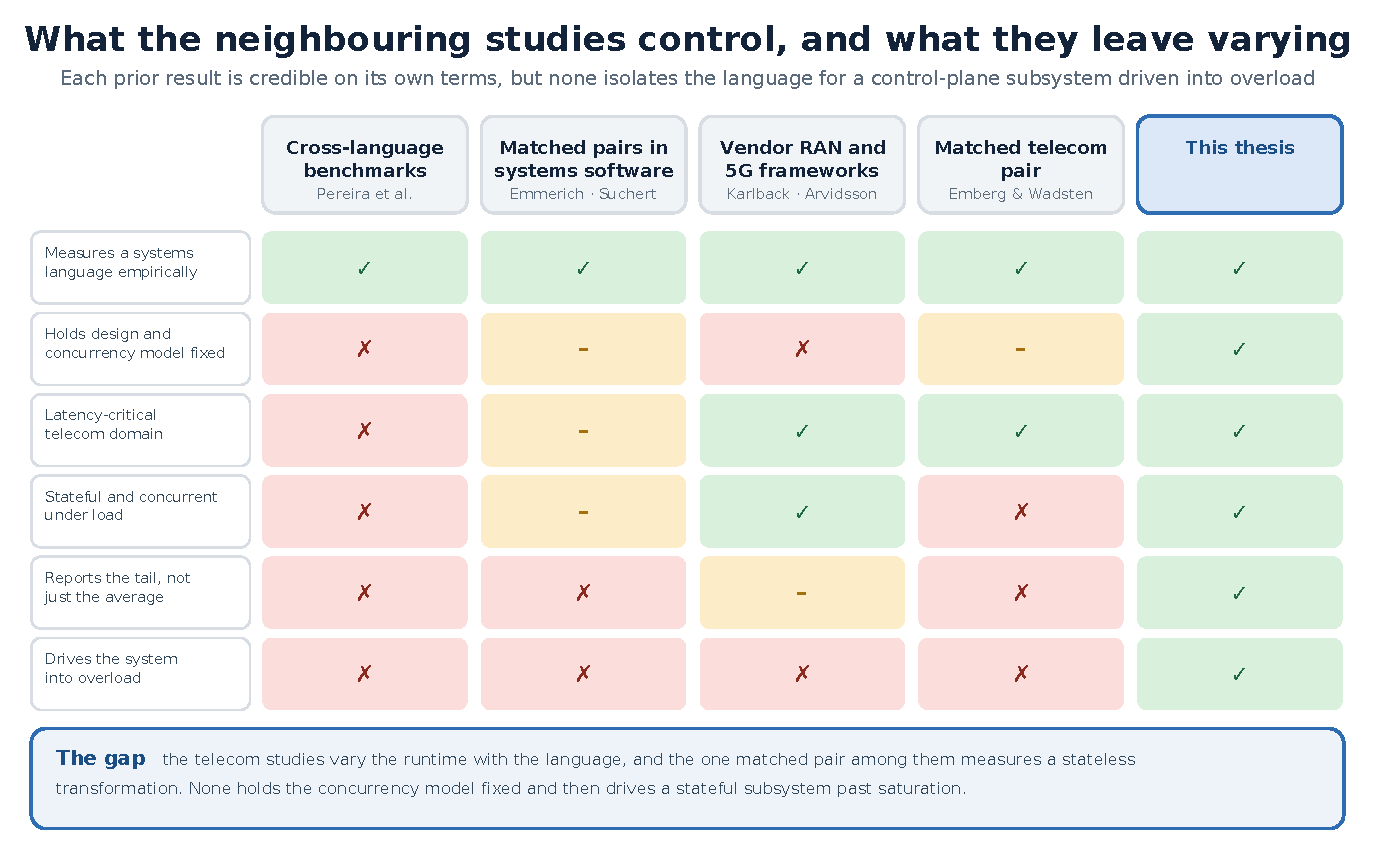
\includegraphics[width=0.78\linewidth]{diagrams/pdf/29_research_gap.pdf}
\caption[What the neighbouring studies control, and what they leave varying]{What the neighbouring studies control, and what they leave varying. Each row is a
property that a controlled answer to the research questions would need. Each column is a study.
The general cross-language comparisons measure the right kind of object but the wrong regime,
reporting averages on general-purpose workloads. Matched pairs in systems software hold the
design fixed, but outside this domain and below saturation. The vendor RAN and 5G framework
studies reach the right domain, and one of them reports the tail, but in all of them the
language varies together with the runtime and the concurrency model. The one matched telecom
pair, Emberg and Wadsten, controls the design but measures a stateless transformation. Holding
the design and the concurrency model fixed for a stateful, concurrent subsystem and then driving
it past saturation is what this thesis adds. The contribution is the control, not a new
measurement technique.\label{fig:gapmap}}
\end{figure}

What is therefore missing from the literature is \emph{direct, controlled} evidence for a
representative control-plane subsystem. The missing comparison is this: Whether Rust actually
holds its tail latency and predictability under overload against modern C++ \emph{when the
concurrency model, algorithms, and data structures are held fixed}. The same gap covers
exactly which defect classes it eliminates and at what stage the remainder are caught, what
its safety model costs in throughput and resources, and what incremental adoption costs in
practice. Closing this gap is the purpose of the four research questions. The next chapter
grounds them in the specific subsystem, defect classes, and timing properties at stake, and
sets out the methodology by which they are pursued.

\chapter{Research Methodology\label{chapter:methodology}}

The preceding chapter set out the gap this study closes. This one sets out how. It begins
with the subsystem the work is carried out on, and with the defect classes and timing
properties at stake in it. It then states the overall research strategy, the method chosen
for each research question and why it is appropriate, the controls that make a language
comparison fair, the statistical treatment of the measurements, and the reproducibility and
ethical commitments under which the work is carried out.

\section{The UE Context Management subsystem}\label{sec:uecm}
The subsystem under study is a UE Context Management service. It is modelled on a real Nokia
gNB-CU-CP service domain that owns the UE context lifecycle, RRC procedure
execution~\cite{3gpp38331}, and mobility and handover. Those are the functions the 3GPP
architecture assigns to the control-plane part of a disaggregated gNB
(Section~\ref{sec:ranarch}). Figure~\ref{fig:fsm} shows the UE-context lifecycle state machine
both implementations encode identically. The mixed workload of Section~\ref{sec:workload}
walks each UE through that machine.

\begin{figure}[ht]
\centering
\begin{tikzpicture}[
    ->, >=Stealth, node distance=3.2cm, font=\small,
    every state/.style={draw, minimum size=1.5cm, fill=blue!6, thick},
    every edge/.style={draw, thick}
  ]
  \node[state, initial, initial text=\scriptsize create] (idle) {Idle};
  \node[state, right=of idle] (conn) {Connected};
  \node[state, right=of conn] (reconf) {Reconf.};
  \node[state, below=1.9cm of conn, fill=gray!10] (rel) {Released};

  \path (idle)  edge node[above,font=\scriptsize]{setup} (conn)
        (conn)  edge[bend left=18] node[above,font=\scriptsize]{begin} (reconf)
        (reconf) edge[bend left=18] node[below,font=\scriptsize]{complete / abort} (conn)
        (conn)  edge node[right,font=\scriptsize,pos=0.45]{release} (rel)
        (idle)  edge[bend right=32] node[below,font=\scriptsize,pos=0.6]{release} (rel);
  \path (conn) edge[loop above] node[font=\scriptsize]{signal / add\_drb} (conn);
\end{tikzpicture}
\caption[UE-context lifecycle state machine]{UE-context lifecycle state machine. \texttt{create} allocates a context in
\texttt{Idle}, \texttt{setup} connects it, and \texttt{signal} and \texttt{add\_drb} are handled
in place while \texttt{Connected}. Operations invalid for the current state return an
\texttt{OpError} instead of changing state.\label{fig:fsm}}
\end{figure}

\paragraph{Why this subsystem.}
UECM is core RAN layer-3 functionality. It carries the properties that make production
control-plane code difficult: per-UE mutable state, a strict operation lifecycle, high
concurrency across UEs, and the latency and reliability targets the 5G system sets for
control-plane procedures~\cite{3gpp38913,3gpp22261}. Conclusions about how a language handles
those properties therefore transfer to other stateful, concurrent control-plane services. It
is also small enough to specify precisely, implement faithfully in two languages, and reason
about in full. That is what makes a parity-tested comparison possible. A larger subsystem would
buy external validity at the cost of the internal validity a fair language comparison depends
on.

\paragraph{Operation set.}
The interface exercised by the study is deliberately small and lifecycle-oriented. It can
create and release a context, set up a connection (\texttt{Idle}$\rightarrow$\texttt{Connected}),
handle an in-session signalling message, add a data radio bearer, begin, complete, or abort a
reconfiguration or handover, and look up a context's state under concurrent load. Every
operation is defined for every state of Figure~\ref{fig:fsm}. An operation illegal in the
current state returns a typed error and leaves the context unchanged, instead of throwing or
corrupting state. That closed, well-typed set lets the same test vectors and the same workload
drive both implementations along identical paths.

\paragraph{The defect classes this subsystem can exhibit.}
RQ2 needs a catalogue and not a list of hazards. One is built from this operation set. It is
$\FaultClasses$ classes in two groups of seven. The split is the falsifiable commitment: seven
drawn from inside the region safe Rust claims to govern, and seven chosen precisely because
safe Rust is expected \emph{not} to prevent them. Each has its expectation recorded before the
programs were run. Every class is mapped to an operation that would exhibit it, so the
catalogue answers to this subsystem and not to memory safety in the abstract.
Section~\ref{sec:safetyresults} reports what each one did.

\paragraph{Why the tail is the metric here.}
Section~\ref{sec:bgbrief} makes the tail the governing quantity for a latency-critical service.
Two properties of this subsystem are why it governs here. One user-visible action, a call
setup or a handover, becomes many dependent control-plane operations. The slowest member gates
completion. A busy site drives thousands of such procedures per second, so a percentile far
out in the distribution is reached often enough to matter. The second is the shape of the
failure. A service of this design tracks its offered load with flat latency until a worker
saturates. Then latency rises by orders of magnitude within one increment of load. That is why
this study sweeps past saturation instead of stopping at a nominal operating point.

\section{Research approach}\label{sec:approach}
The study is experimental with a constructive (design-science) element. The artifact is a pair
of functionally equivalent implementations of the subsystem, one in C++ and one in Rust,
plus the framework that benchmarks them. Both are built from a single frozen specification
and then evaluated under controlled experiments. Evidence is triangulated across three
methods. Performance measurement under a load sweep answers RQ1 and RQ3. A controlled
fault-injection study answers RQ2. An FFI migration case study, part measured and part
qualitative, answers RQ4. A weakness in one of them, such as the environment sensitivity of tail-latency
measurement, therefore does not carry into the conclusions as a whole, because the three methods are independent of each other. Every measurement reports variance over repeated runs.
Section~\ref{sec:controlsbrief} sets out the controls that keep the language the only variable.

That design follows from the shape of the questions. Each asks how one outcome (tail latency,
defects prevented, resource use, migration cost) depends on one variable, the implementation
language. The language therefore has to be the only systematic difference between the two
objects under test. This rules out the commonest form of language comparison in the literature,
where two independently written programs are measured and the gap is attributed to the
language. Such a gap also carries the design, the libraries and the skill of their authors.

Building both sides from one specification removes that confound. The comparison is then between
two encodings of the same design, and the artifact becomes both the contribution and the
instrument that measures it. Where a question can be answered with numbers, the treatment is
quantitative. Where it cannot, as with the kind of guarantee in RQ2 and the application
programming interface (API) design effort in RQ4, it is qualitative but still systematic.

The gap this design addresses (Section~\ref{sec:gap}) is only as good as the search that looked
for it, so that search is on record. Appendix~\ref{appendix:search} gives the databases, the term
combinations, the citation chaining and the filtering rules. Two of its findings bear on the
design and not just on the bibliography.

The vendor-hosted theses closest to this study appear in no
citation database. Chaining therefore never reaches them, and they had to be found by searching
the institutional repositories directly. The same searches establish an absence on the other
side: no Finnish thesis on Rust in a radio-access or telecom context, and no indexed publication
mentioning Rust from the vendor hosting this work. The domain-specific literature on the
language question is therefore Swedish and Ericsson-hosted, and whether it carries over here is
untested. Those theses are grey literature, so they are cited as evidence of what a vendor has
attempted and found, not as peer-reviewed results.

The search returned no study, indexed or grey, that measures the tail-latency behaviour of a
Rust and a C++ implementation of the same stateful, concurrent control-plane subsystem under
overload.

Table~\ref{tab:design} maps each research question to the method, artifact, data and metric
that answer it. All four chains end in the same place. Section~\ref{sec:rqdiscussion} judges
each question and Section~\ref{sec:hypotheses} disposes of its hypothesis. RQ1 and RQ3 share
H1, worded to cover performance equivalence in both the latency and the resource sense. That
wording turns out to be the hypothesis's main weakness. RQ2 is insensitive to the
environment. RQ4 is so except along one axis: build time is a timing measurement like any
other, and is therefore read as a ratio between two toolchains measured alternately on one
machine. RQ1 and RQ3 depend on the measurement host and are reported against what it can carry
(Section~\ref{sec:testbed}).

\begin{table}[H]
\centering
\caption[Research design: how each research question is answered]{Research design: how each research question is answered. Every question is tied to a
concrete method, a published artifact, the data it produces, and the metric on which the
conclusion rests. RQ1 and RQ3 carry two methods rather than one: the sweep measures the
round-trip a deployment would experience, and the component decomposition measures the part of
it the language is responsible for. Section~\ref{sec:methodbrief} states why one cannot stand in
for the other. RQ1 and RQ3 are tested against H1, RQ2 against H2, and RQ4 against H3. The RQ2 row
abbreviates the three dynamic sanitisers the C++ side is built under: AddressSanitizer (ASan),
ThreadSanitizer (TSan) and UndefinedBehaviorSanitizer
(UBSan).\label{tab:design}}
\renewcommand{\arraystretch}{1.25}
\begin{tabular}{@{}p{0.06\linewidth} p{0.24\linewidth} p{0.24\linewidth} p{0.32\linewidth}@{}}
\hline\hline
RQ & Method & Artifact / data & Primary metric \\
\hline
RQ1 & Load sweep to overload, interleaved repeats & Benchmark harness, latency histograms &
median, p99/p99.9/p99.99 tail latency, and maximum vs.\ offered load \\
RQ3 & Same sweep, resource capture & \texttt{getrusage} samples per run &
peak resident set size (RSS), CPU utilisation, throughput \\
RQ1, RQ3 & Component decomposition: the core called directly, then through the service &
Matched microbenchmark pair, interleaved repeats &
per-operation cost split into the operation and the cross-thread handoff \\
RQ2 & Controlled fault injection & Defect catalogue, ASan/TSan/UBSan, \texttt{rustc},
Loom/Shuttle and Miri logs &
defect-class taxonomy (compile-time / runtime / undetected) \\
RQ4 & FFI migration prototype & C++ host $+$ Rust C-ABI seam &
seam size, \texttt{unsafe} scope, per-call interop cost \\
\hline
\end{tabular}
\end{table}

\section{Methods per research question, in outline}\label{sec:methodbrief}
RQ1 and RQ3 are answered by an open-loop load sweep from light load to well past saturation.
The four build variants are interleaved inside every repeat. A second measurement separates the
operation from the cross-thread handoff around it. The end-to-end round-trip bundles two costs
of different character, and only one of them can differ between the languages. A third
isolates the contended queue and completion primitives on their own, so the overload
attribution can be tested and not merely argued.

RQ2 is answered by controlled fault injection. Each defect class is written as a small
self-contained program in both languages. The C++ side is built and run under
AddressSanitizer, ThreadSanitizer and UndefinedBehaviorSanitizer. The safe-Rust side is
compiled and, where it compiles, run under a bounded timeout. No static analyser is run,
deliberately. The C++ columns therefore report the tooling this study ran and not a ceiling on
what C++ tooling could find. RQ4 is answered by a working migration prototype in the direction
a real migration takes: a C++ host calling an unmodified Rust core across a C application
binary interface. The per-call cost is measured on a real operation and not inferred from an
empty crossing.

\section{Fairness as a controlled variable}\label{sec:controlsbrief}
A language comparison is only as good as the variables it holds fixed. The specification is
frozen before either implementation exists. The concurrency model, the allocator and its arena
count, the optimisation level, the hash function, the histogram algorithm and the load schedule
are matched across the two sides, never tuned per side. Where the two languages could not be
written alike the divergence is logged instead of resolved. Behavioural equivalence is
established by diffing conformance transcripts operation by operation. One row of that table
has no control against it: one person wrote both implementations and is not equally expert in
both. Section~\ref{sec:standing} treats that as the study's principal internal threat.

\section{Statistical treatment}\label{sec:statsbrief}
The statistical design is fixed in advance, because the study's credibility rests on that.
The family of tested comparisons is enumerated ahead of the campaign, so an operating point
identified after seeing a sweep cannot enter it however small its $p$-value would be. Each
comparison is an exact paired permutation test over \NRepeats{} interleaved repeats with a
bootstrap confidence interval, Holm-corrected across the family. The attainable floors
($\MinAttainableP$ uncorrected, $\CorrectedFloor$ corrected) are quoted so that a null can be
distinguished from an arithmetic limit. Two quantities are deliberately excluded from the
family. One is inter-operation jitter, which no research question asks for. The other is the
pooled p99.99 far tail, whose unit of analysis is the operation and not the run, so it has no
across-repeat interval to test.

\section{Reproducibility and research artifacts}\label{sec:repro}
A third party can regenerate the results without access to Nokia's proprietary code, for
three reasons. The implementations are driven entirely by the public frozen specification. The
benchmarking harness, the fault catalogue and its runner, and the FFI prototype are published
together with the thesis. Every result table, every plot of measured data, and every quoted
number in the evaluation is rebuilt by one regeneration script in the published package
(\texttt{bench/refresh\_thesis.sh}) directly from the raw logs. The scope of that claim is
worth stating precisely. Two things it might be read to cover are outside it. The hand-drawn
schematics that explain a concept rather than report a result are authored and not generated.
And running the same scripts over another host's campaign regenerates the artifacts by the
same procedure and not with the same values. What the script guarantees is that no figure,
table, or sentence can hold a value the logs no longer support.

The logs that script reads are part of the package. A performance campaign is an append-only
newline-delimited JavaScript Object Notation (JSON) file, named by the timestamp at which it
started. The reported sweep and the virtualised campaign it replaced both sit under
\texttt{bench/results/}, while the second bare-metal campaign has a directory of its own. Each
campaign has its own script and its own macro prefix, so a figure from one cannot reach a
sentence about another. The two bare-metal campaigns also write a sidecar holding every run's
complete histogram buckets. The far-tail percentile is computed from those buckets, which the
virtualised campaign predates. Each run's environment is recorded by
\texttt{bench/capture\_env.sh} and stored beside the campaign data. Three runners write three
machine-readable outcome files under \texttt{faults/results/}: \texttt{taxonomy.csv},
\texttt{model\_checking.csv}, and \texttt{miri.csv}. Nothing in the evaluation chapters is
transcribed from those files by hand. The execution environment travels with its data, which
is what lets the thesis separate environment-sensitive results from environment-insensitive
ones. Nothing on the path requires proprietary source.

\section{The two implementations in brief}\label{sec:designbrief}
The properties of the design and of both implementations that the evaluation depends on are
these. Both are built from one frozen specification, written before either implementation
existed. That specification fixes the operation set, the state machine and the error model
before either version could negotiate them. Both use the same concurrency structure: a
shared-nothing thread-per-shard pool in which each worker owns its slice of the UE state
outright, reached through a bounded blocking queue of fixed capacity. No lock protects shared
mutable state on the hot path in either language. A request crosses that queue as a tagged value
carrying a one-shot completion handle. That is what makes the end-to-end latency a
submit-and-complete round-trip and not a function call.

Where the two could not be written the same way, the divergence is logged and left unresolved
in either direction. Two of those divergences carry the overload result of
Section~\ref{sec:overload}: the bounded queue, hand-written in C++ against Rust's
\texttt{sync\_channel}, and the completion handle, \texttt{std::promise} against a fresh
\texttt{mpsc} channel per request. A third carries the operation-level result of
Section~\ref{sec:budget}, since the per-shard container is each language's own standard hash map
and those are different data structures. The hash function itself is pinned to the
Fowler--Noll--Vo hash function (FNV-1a) on both sides precisely so that hashing cannot be the
explanation. Behavioural equivalence is not assumed either. A language-neutral conformance
suite drives both through $\ConfHandOps$ hand-written and $\ConfGenOps$ generated operations
and diffs the canonical transcripts operation by operation.

\chapter{Experimental Setup and Evaluation\label{chapter:eval}}

The chapter first names the machines and the workload, then reports the results. Setup
questions (what was pinned, what was not) come before any comparison. The findings themselves
are grouped by research question.

\section{Testbed configuration\label{sec:testbed}}
This chapter reports two kinds of result. Some follow from the compilers and the source. Others
depend on the machine. Table~\ref{tab:testbed} describes the machines and keeps that split clear.

Every performance number here comes from one dedicated bare-metal server: a single-socket
\MainCpu{} with \MainCores{} cores on \MainNumaNodes{} non-uniform memory access (NUMA) node,
simultaneous multithreading (SMT) \MainSmt{}, running \MainHostDistro{} on kernel \MainKernel{}.
The frequency governor is fixed
at \MainGovernor{} with boost disabled, so the cores hold their base clock, and cores \MainPinned{}
carry the benchmark. The environment capture records virtualisation as \MainVirt{}, and every run
records the metadata of Section~\ref{sec:repro}.

The toolchain is not the host's. Both implementations are built and run inside a pinned container
image carrying \MainDistro{} with \texttt{g++~\MainGpp} and \texttt{rustc~\MainRustc}, the same
image and the same \texttt{rustc} the earlier virtualised campaign used. The image pins the
\texttt{gcc-toolset} major version and not the release within it, so that campaign compiled with
\texttt{g++~\GuestGpp}, one GCC~15 release earlier. The container also takes the kernel from its
host. The two campaigns therefore differ in the hardware, in the kernel (\MainKernel{} against
\GuestKernel{}), and in that compiler release.

Two properties of this host are what the previous one lacked. No hypervisor sits between the
benchmark and the cores, so no timeslice is lost to a machine this study cannot observe. The
kernel runs tickless on the pinned cores (\texttt{nohz\_full}), which removes the periodic timer
interrupt from the measured path. What the host does \emph{not} have is \texttt{isolcpus},
deliberately. Isolating cores also removes them from every scheduling domain. The benchmark
pins its threads to a range and relies on the kernel to spread them, so an isolated set
collapses all of them onto one core. Section~\ref{sec:standing} records the cost.

Until late in the work the campaign ran on a virtualised host instead: a \GuestCpu{} guest,
\GuestCores{} vCPUs, \GuestVirt{} virtualisation, no core isolation. Three of this chapter's
results were already settled there. One was not settleable there at all, and the obstacle was
not a shortage of repeats. On that host the $95\%$ confidence interval on a single variant's p99
spans $\GuestPNineNineMaxCI\,\mu$s, while the four variants' p99 values differ by
$\GuestPNineNineRange\,\mu$s. The uncertainty about one swamped the gap between all of them.
That campaign is not discarded. It shares this one's design exactly: the same \GuestShards{}
shards and \GuestProducers{} producers over \GuestLoadLevels{} load levels at \GuestRepeats{}
repeats. The two can be set side by side to ask which findings belong to the code. That
comparison is the only direct evidence this study can offer that its instrument is adequate to
the questions it asks. One of its findings is that a quantity this thesis once reported as a
property of allocators was in part a property of that machine.

On either host Section~\ref{sec:statsbrief} applies. Each sweep point is a median over
\NRepeats{} interleaved repeats with a bootstrap $95\%$ confidence interval. Interleaving shares
interference across variants, which costs absolute latency and preserves the comparison.
Throughput is counted over the measured phase only, warm-up excluded.

\section{Workload and evaluation measurements\label{sec:workload}}
A synthetic but spec-justified telecom workload is generated by a deterministic driver whose
structure both implementations share, so the two versions are exercised along identical code
paths. The \emph{signal} workload preloads a population of connected UEs and hammers the
\texttt{handle\_signalling} hot path. That isolates steady-state per-message latency. The
\emph{mixed} workload walks each UE through a realistic procedure sequence: context creation,
connection setup, signalling, bearer setup, reconfiguration or handover (begin, complete, or
abort), and release. A fixed SplitMix64 draw order and a per-slot expected-state model keep
every operation it emits valid. The fixed draw order makes the per-operation-kind counts
identical in C++ and Rust for a given active-UE population and seed. That doubles as the
parity signal of Section~\ref{sec:designbrief}. The control parameters are the target event rate
and the number of active UEs, swept from nominal load through saturation and overload. The send
schedule is fixed and the histogram is corrected, so a stall introduces no coordinated-omission
bias~\cite{schroeder2006openclosed,tene_hdrhistogram}. Three campaigns are run: a load sweep for
performance, the fault-injection study, and an FFI migration prototype.
Figure~\ref{fig:workload} shows the two workloads and the sequence the mixed one walks.

\begin{figure}[ht]
\centering
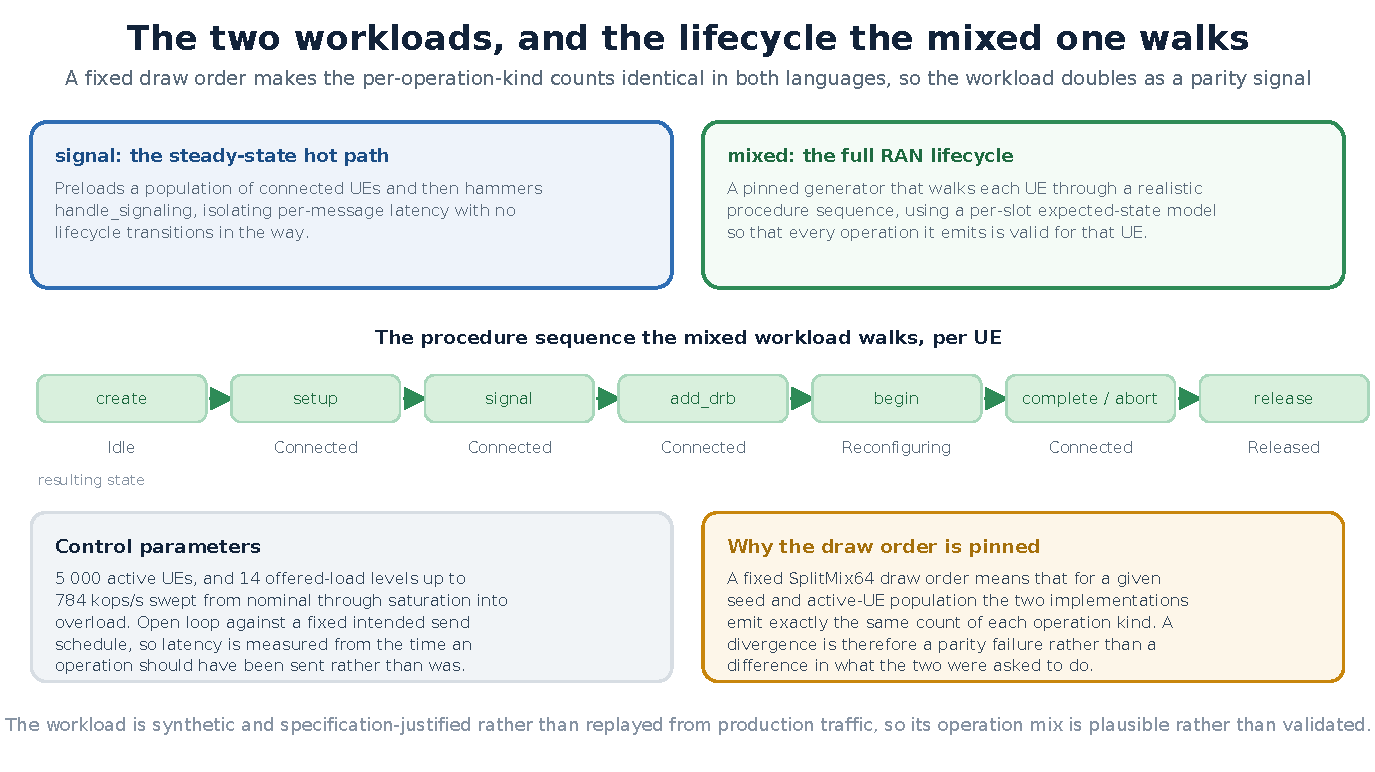
\includegraphics[width=0.78\linewidth]{diagrams/pdf/27_workload_timeline.pdf}
\caption[The two workloads, and the lifecycle the mixed one walks]{The two workloads. The \emph{signal} workload isolates the steady-state hot path.
The \emph{mixed} workload walks each UE through the full RAN procedure sequence, with a
per-slot expected-state model ensuring that every operation it emits is legal for the state
its context is actually in. Because the SplitMix64 draw order is pinned, a given seed and
active-UE population produce identical per-operation-kind counts in both languages, so a
divergence is a parity failure rather than a difference in what the two implementations were
asked to do.\label{fig:workload}}
\end{figure}

The term \emph{spec-justified} is used precisely, because the distinction bounds what the
workload can support. The \emph{sequence} of operations is justified. It is the RRC connection
lifecycle the 3GPP specifications define for a UE, from establishment through in-session
signalling and bearer setup to reconfiguration and release~\cite{3gpp38401,3gpp38331}. The
per-slot expected-state model guarantees that every operation the driver emits is legal for the
state its context is in. The \emph{proportions} are not justified in the same way. How often a
real cell hands over, against how often it establishes a bearer, depends on deployment, mobility
and time of day. No public figure fixes it, so the mix used here is plausible and not
validated. Section~\ref{sec:standing} reports that as a threat to external validity, and trace
replay heads the future-work list for it. For a \emph{comparative} question it costs less than it
would for an absolute one. Both implementations execute the same sequence in the same order for a
given seed and active-UE population, verified by the per-operation-kind counts. An
unrepresentative mix therefore shifts both languages equally and cannot manufacture a difference
between them. It bounds how far the numbers travel and not the fairness of the comparison.

Table~\ref{tab:params} gathers the configuration of the service, the workload and the campaign in
one place, since those values are otherwise spread across the specification,
Section~\ref{sec:designbrief} and this chapter. Every entry in the campaign block is either fixed
by the specification or generated from the measurement logs. Two operating points are used
throughout. The first of them is fixed in advance, not derived from the data. The
representative point sits at $\ReprLoad$~kops/s against a measured throughput plateau of
$\SatKnee$~kops/s. It is fixed because the alternative was tried and failed. The rule this study
began with took the busiest swept load at which all four variants still held their p99 below
$5$~ms. It is retained as a diagnostic and is no longer the operating point, because it measures
the machine and not the service. On the virtualised host it returned $\GuestDeadlineLoad$~kops/s,
where p99 sat just under the deadline, so it was locating where that host's interference reached
$5$~ms. On a quiet host p99 stays near $\PNineNineTrackingTop\,\mu$s until capacity binds, so the
same rule climbs until it collapses the representative point onto the saturation knee. Fixing
the point costs the appearance of derivation. It buys two things worth more: the hosts are
compared at the same offered load, and the point stays below saturation on all of them, which
every below-saturation claim in this chapter assumes.

\section{Evaluation data}\label{sec:evaldata}
The campaigns behind this chapter differ in kind: one load sweep, three small paired
experiments, a categorical fault catalogue, a build and footprint measurement, and two further
sweeps kept for comparison. Appendix~\ref{appendix:config} records what each captured, field by
field, because judging the analysis takes knowing the record and not only the tables drawn from
it. Every measured quantity this chapter quotes is a generated macro
(Section~\ref{sec:repro}). The software-quality proxies sit beside the forced divergences they
explain, and beside the FFI seam, the only place either implementation contains \texttt{unsafe}
(Table~\ref{tab:ffi}).

\section{Evaluation results}
The safety and most of the migration results do not depend on the measurement host. The
performance and resource results do. Every figure and table below is measured on the host of
Section~\ref{sec:testbed} unless stated otherwise. Every comparison on that host resolves,
including the far tail below saturation. The divergence past saturation is resolved as a
measurement and not as a mechanism. Section~\ref{sec:contention} reports how far the mechanism
could be narrowed.

\subsection{Below saturation (RQ1, RQ3)}\label{sec:perfresults}
The hypothesis under test is H1 (Section~\ref{sec:rqs}): equivalence below saturation, with any
difference confined to the far tail. Each point aggregates \NRepeats{} interleaved repeats.
Reported values and shaded bands are medians with nonparametric bootstrap $95\%$ confidence
intervals. Table~\ref{tab:latency} summarises per-operation latency at the representative load of
Section~\ref{sec:workload}, $\ReprLoad$~kops/s, a point at which all four build variants are
simultaneously healthy.

Two readings of that table answer different questions. Magnitude is negligible: the four variants
sit within $\PFiftyRange\,\mu$s of one another at the median, $\PFiftySpread\%$, which no
deployment would notice. \emph{Ordering} is legible: the two Rust intervals sit below the two C++
intervals with no overlap between the languages, while the two allocators of one language overlap
each other. On the previous host every interval at this percentile overlapped every other, and the
ordering had to come from the test alone. That agreement extends up the distribution. The p99
values differ by $\PNineNineRange\,\mu$s across variants, while the widest $95\%$ confidence
interval on a single variant's own p99 spans $\PNineNineMaxCI\,\mu$s. The uncertainty about one
variant is smaller than the gap between them, which is what licenses an ordering. It is also the
relation this study could not obtain for most of its life. On the virtualised host the same two
quantities were $\GuestPNineNineRange\,\mu$s and $\GuestPNineNineMaxCI\,\mu$s, the wrong way round
by a factor of five. That is a result about measurement rather than about either language.

The tail rows of Table~\ref{tab:significance} therefore carry a finding. The instrument that
carries it is the corrected $p$-value and not the interval. Both p99 rows and both p99.9 rows
clear the Holm correction, \NTailSignificant{} rows in all, in the same direction as at the median.
Their intervals also exclude zero. Section~\ref{sec:statsbrief} fixes in advance that an interval
in this block is not read as a finding, so those are reported and left to one side. A rule dropped
once the machine improves was never a rule.

Predictability is evidenced as far as p99.99. That column is a different statistic from the
rest of its table: one percentile of the \NRepeats{} repeats' histograms concatenated, between
\FarTailSamplesMin{} and \FarTailSamplesMax{} operations per variant, which is what
Section~\ref{sec:statsbrief} means by pooling. A single run holds too few observations past p99.99
for the percentile to mean anything. Every run persists its full histogram buckets so the repeats
can be combined afterwards. Pooling takes the operation as the unit of analysis, so the column
has no across-repeat interval and none is printed. Read that way the far tail separates the
languages outright. The widest gap between variants is $\FarTailRange\,\mu$s,
$\FarTailSpread\%$ of the smallest, and both \FarTailLower{} variants sit below both of the
others.

\begin{table}[H]
\centering
\small
\caption[Per-operation latency (\textmu s) at the representative load]{Per-operation latency, in microseconds, at a sustained
offered load of $\ReprLoad$~kops/s (mixed RAN-lifecycle workload, $7$ shards). The median over
\NRepeats{} repeats is printed above its nonparametric bootstrap $95\%$ confidence interval. The
interval is printed in full rather than as a symmetric half-width because it is strongly
asymmetric at these percentiles and a half-width covering the upper bound would place the lower
one below zero. $^{\dagger}$The p99.99 column is the deliberate exception, one percentile of the
\NRepeats{} repeats' histograms concatenated, \FarTailSamplesMin{} to \FarTailSamplesMax{}
operations per row, because a per-run p99.99 rests on too few observations to read. Pooling makes the operation the unit of analysis, so that column
carries no across-repeat interval. With the maximum it is one of the two columns the paired
family does not test, for the same reason: both are read off exactly the operations interference
lands on, which is the class pairing cannot rescue.\label{tab:latency}}
% Tabular preamble and header are generated alongside the table body, so the table
% gains a p99.99 column when a campaign records one instead of the preamble falling
% one column short of the body it is wrapping. \LatencyTabular expands to the whole
% \begin{tabular}{...}: array's preamble scanner does not expand macros, so passing
% only the column specification would fail with "Illegal pream-token".
\LatencyTabular
\hline\hline
\LatencyHead \\
\hline
C++ (system alloc) & \mci{217.2}{163.8}{237.2} & \mci{355.1}{289.3}{389.4} & \mci{674.3}{395.3}{1538.0} & \mci{2170}{910}{5594} \\
C++ (jemalloc) & \mci{225.8}{181.1}{261.2} & \mci{410.1}{305.7}{11280.4} & \mci{1188}{544}{14213} & \mci{3590}{1472}{16291} \\
Rust (system alloc) & \mci{214.3}{191.6}{238.8} & \mci{376.3}{330.2}{3629.1} & \mci{1068}{504}{6955} & \mci{2404}{1129}{9667} \\
Rust (jemalloc) & \mci{208.4}{193.7}{223.1} & \mci{388.9}{342.3}{478.0} & \mci{763.4}{479.5}{4272.1} & \mci{2804}{1114}{7606}
\\
\hline
\end{tabular}
\end{table}

Those percentiles describe the distribution and not how far consecutive operations differ from
each other. Request for Comments (RFC)~3393 names that inter-operation delay
variation~\cite{rfc3393}. Table~\ref{tab:jitter} in Appendix~\ref{appendix:config} reports it
descriptively, because no research question asks for it. Median jitter across the four variants
runs $\JitterLo$ to $\JitterHi\,\mu$s, $\JitterVsMedianPct\%$ of the median latency it perturbs.
What separates the four variants is smaller than what separates one load level from the next,
the conclusion the second bare-metal campaign reaches independently.

Overlapping intervals are a weak instrument in both directions, so the comparison is also tested
directly, by the procedure fixed in Section~\ref{sec:statsbrief} and reported in
Table~\ref{tab:significance}. What licenses the pairing is a property of this campaign rather
than of the statistic. The four variants are interleaved inside every repeat, so the $i$-th run
of each met the same ambient conditions. Whatever interference that block carried cancels in their
difference. That is the second thing the interleaving discipline buys, beyond the fairness
argument it was adopted for.

\begin{table}[tp]
\centering
\small
\caption[Exact paired permutation test of C++ against Rust]{Exact paired permutation test of C++ against Rust at $\ReprLoad$~kops/s, with the
allocator held fixed. The effect is the median of the \NRepeats{} paired differences
(Rust~$-$~C++) above its bootstrap $95\%$ confidence interval, the test statistic is their mean,
$p$ is exact over all $2^{\NRepeats}$ sign assignments, and the final column applies the Holm
correction across the whole family of \NTests{} tests. The attainable floors are
$\MinAttainableP$ uncorrected and $\CorrectedFloor$ after correction. The rows are blocked by the
criterion of Section~\ref{sec:statsbrief}: pairing rescues the statistics in the upper block, so a
consistent interval there is evidence, whereas the high percentiles below are computed from
exactly the operations interference falls on, so an interval excluding zero is not read as a
finding. Both blocks clear the correction here, so the rule costs the lower block nothing and is
applied anyway. Achieved throughput is not tested, for the reason given in the same section, and
appears in Table~\ref{tab:resource} instead.\label{tab:significance}}
\begin{tabular}{@{}l l r r r@{}}
\hline\hline
Metric & Allocator & Effect (Rust $-$ C++) & $p$ & Holm \\
\hline
\rlap{\emph{Robust to interference on single operations}} & & & & \\
p50 latency (\textmu s) & system & \mci{-1.3}{-1.3}{-1.2} & 0.0000019 & 0.000027 \\
p50 latency (\textmu s) & jemalloc & \mci{-1.2}{-1.3}{-1.2} & 0.0000019 & 0.000027 \\
Peak RSS (MiB) & system & \mci{+1.4}{+1.2}{+1.7} & 0.0000019 & 0.000027 \\
Peak RSS (MiB) & jemalloc & \mci{+2.5}{+2.4}{+2.6} & 0.0000019 & 0.000027 \\
CPU utilisation (\%) & system & \mci{-5.1}{-6.7}{-4.7} & 0.0000019 & 0.000027 \\
CPU utilisation (\%) & jemalloc & \mci{-4.6}{-5.9}{-3.9} & 0.0000019 & 0.000027\\
\hline
\rlap{\emph{Determined by it: high percentiles}} & & & & \\
p99 latency (\textmu s) & system & \mci{-1}{-2}{-1} & 0.0000057 & 0.000027 \\
p99 latency (\textmu s) & jemalloc & \mci{-1}{-1}{-1} & 0.0000038 & 0.000027 \\
p99.9 latency (\textmu s) & system & \mci{-4}{-5}{-2} & 0.00016 & 0.00016 \\
p99.9 latency (\textmu s) & jemalloc & \mci{-2}{-4}{-2} & 0.0000095 & 0.000027
\\
\hline
\end{tabular}
\end{table}

\begin{figure}[ht]
\centering
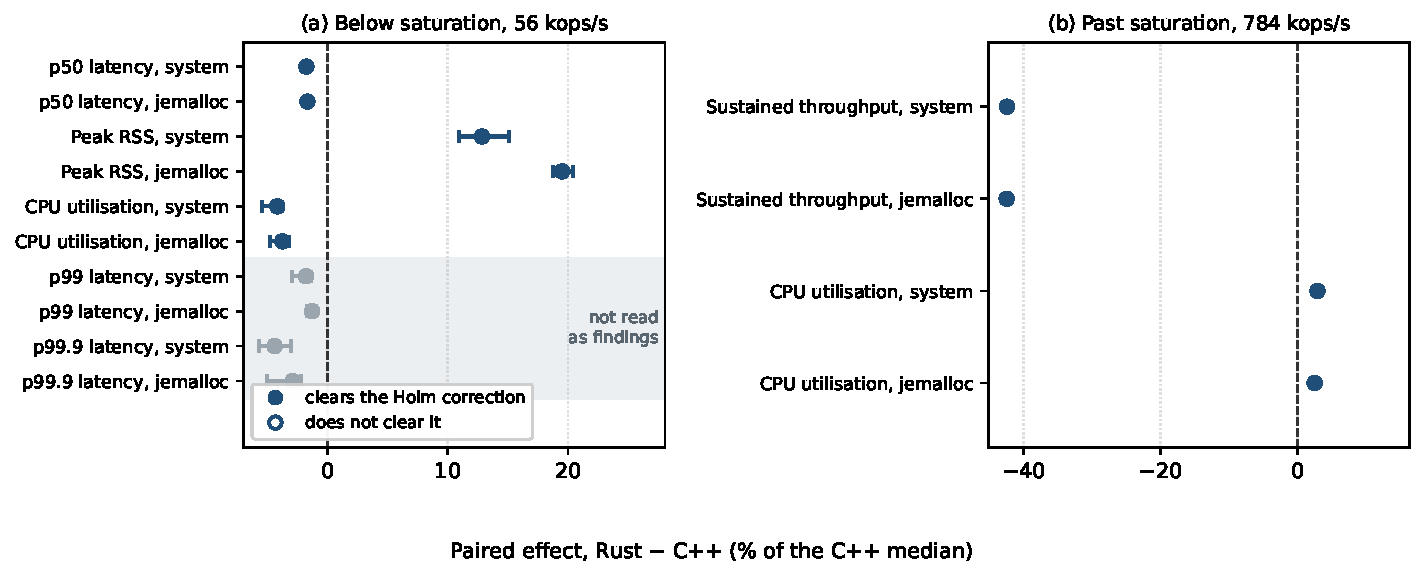
\includegraphics[width=0.78\linewidth]{figures/fig_effects.pdf}
\caption[The tested family drawn as paired effects]{Every test in Tables~\ref{tab:significance} and~\ref{tab:overloadtest} as a paired
effect with its bootstrap $95\%$ interval, normalised by the C++ median so that microseconds,
mebibytes, percentage points and kops/s can share an axis. Filled markers are the
\NSignificant{} of \NTests{} tests that clear the Holm correction, which here is all of them. The
two allocators of a metric are drawn adjacent, so an effect that reversed sign between them would
appear as a pair straddling the zero line. The shaded rows are the high percentiles, which
Section~\ref{sec:statsbrief} fixes in advance as rows whose \emph{intervals} are not read as findings.
Their corrected $p$-values are read, so the shading marks the instrument that is set aside and
not the rows.\label{fig:effects}}
\end{figure}

Figure~\ref{fig:effects} draws the same family on one axis. All \NSignificant{} of the \NTests{}
tests survive Holm, none changes sign when the allocator changes, the tail intervals are the
widest of the set, and the smallest adjusted value sits at the family's own floor of
$\CorrectedFloor$. A family in which nothing fails invites the objection that the threshold is
doing no work: peak resident set size under \texttt{jemalloc} did not clear it on the virtualised
host, and neither did any tail row there. \NExclZero{} paired intervals exclude zero across both
blocks, so the reading rule of Section~\ref{sec:statsbrief} changes no verdict, and an earlier
seven-repeat pass produced tail intervals excluding zero that more repeats removed. The allocator
control runs every comparison twice, and here \CrossAllocConsistent{} keep their sign and
\NCrossAllocReversed{} reverse. Section~\ref{sec:standing} records the campaign on which the
control did veto.

Resolving a difference is not the same as sizing it, and Table~\ref{tab:equivalence} is where the
size goes. Every row is significant here, so the verdict column carries no information and the
margins carry all of it: at the median the effect could be no larger than
$\EqvBoundPFifty\,\mu$s, and in the tail block no larger than $\EqvBoundTailMax\,\mu$s, both
below anything a procedure budget of a few milliseconds would notice. The differences are real,
reproducible and operationally negligible. That table was built to report the opposite case, and
on the virtualised host it did, with \GuestNEqvUnresolved{} of its \GuestNEqvRows{} rows
unresolved and a tail margin running out to $\GuestEqvBoundTailMax\,\mu$s.

\begin{table}[tp]
\centering
\small
\caption[How large each effect could be]{How large each effect could be. For every comparison at
$\ReprLoad$~kops/s, the observed effect against the tightest margin within which the two variants
could be called equivalent, and the verdict Table~\ref{tab:significance} reaches. The two
questions are kept in separate tables on purpose: one asks whether a difference is there, this
one asks how large it could be, and a row can matter in one and not the other. Every row resolves
on the host reported here, so the last column reads the same throughout and the margins carry the
information. On the virtualised host this study measured on first,
\GuestNEqvUnresolved{} of these rows did not resolve, which is what the table was built to
report. Latency margins are in microseconds, peak resident set size in mebibytes, CPU utilisation
in percentage points.\label{tab:equivalence}}
\begin{tabular}{@{}l l r r l@{}}
\hline\hline
Metric & Allocator & $|$Effect$|$ & Equivalent within & Verdict \\
\hline
p50 latency (\textmu s) & system & 1.2 & 1.3 & significant \\
p50 latency (\textmu s) & jemalloc & 1.5 & 1.6 & significant \\
p99 latency (\textmu s) & system & 2 & 2 & significant \\
p99 latency (\textmu s) & jemalloc & 1 & 1 & significant \\
p99.9 latency (\textmu s) & system & 4 & 4 & significant \\
p99.9 latency (\textmu s) & jemalloc & 3 & 3 & significant \\
Peak RSS (MiB) & system & 1.6 & 1.8 & significant \\
Peak RSS (MiB) & jemalloc & 2.5 & 2.5 & significant \\
CPU utilisation (\%) & system & 6.0 & 7.1 & significant \\
CPU utilisation (\%) & jemalloc & 6.2 & 7.3 & significant
\\
\hline
\end{tabular}
\end{table}

The median itself is a resolved difference and not a null: $\PFiftyDiffAbsMax\,\mu$s
in Rust's favour, consistent under both allocators. The interval on it reaches
$\PFiftyDiffCIMax\,\mu$s against a median of $\PFiftyMedian\,\mu$s. The temptation is to report
that as a bound on the language effect. That reading would be wrong, for the reason set out
next.

\paragraph{What the end-to-end number is made of.}\label{sec:budget}
Every latency the sweep reports is an end-to-end round-trip. Section~\ref{sec:methodbrief} set
out why that bundles two costs of quite different character. One is the operation itself, executed
inside a single thread and generated by the compiler. The other is the cross-thread
submit-and-complete handoff around it, charged to the operating system. Only the first can
plausibly differ between the languages. The sweep cannot separate the two, and a bound says only
as much as the quantity it is a fraction of. Both costs are therefore measured directly by the
two-level method described there, in both languages and at the sweep's own shard count and
context population. \texttt{ShardCore} with no queue in the path gives the operation.
\texttt{Service} gives the operation plus the handoff. Their difference is the handoff.
Table~\ref{tab:budget} reframes the whole performance comparison.

\begin{table}[tp]
\centering
\small
\caption[Where an end-to-end operation's cost actually goes]{Where an end-to-end operation's cost actually goes, measured at $7$ shards and
$5\,000$ active UEs with a single uncontended caller. Each row is the median over
\BudgetRepeats{} interleaved repeats above its bootstrap $95\%$ confidence interval, in the
unit its own magnitude calls for: the two terms differ by more than two orders of magnitude,
which is the point of the table. $p$ is the exact two-sided paired permutation test of C++
against Rust on the repeat-wise differences. The handoff is obtained as the difference between
the two measured rows, so it carries the uncertainty of both. It predates the move to bare metal and
carries no environment record, so the absolute nanoseconds name no host. Both arms ran alternately in
one session, which is what the share and the ratio rest on.\label{tab:budget}}
\begin{tabular}{@{}l r r r@{}}
\hline\hline
Component & C++ & Rust & $p$ \\
\hline
Operation alone, no queue in the path (ns) & \mci{34.4}{32.5}{34.5} & \mci{21.3}{21.0}{22.5} & 0.000061 \\
Cross-thread submit-and-complete handoff (\textmu s) & \mci{13.49}{13.36}{13.64} & \mci{12.61}{12.37}{12.89} & 0.227 \\
End-to-end round-trip, uncontended (\textmu s) & \mci{13.52}{13.39}{13.68} & \mci{12.63}{12.39}{12.91} & 0.215 \\
Operation's share of the round-trip & 0.250\,\% & 0.170\,\% & 
\\
\hline
\end{tabular}
\end{table}

The operation is $\BudgetCoreCpp$~ns in C++ and $\BudgetCoreRust$~ns in Rust, and the handoff
$\BudgetHandoffCpp\,\mu$s against $\BudgetHandoffRust\,\mu$s. The work the languages actually
perform is therefore at most $\BudgetCoreShareMax\%$ of what the sweep measures, and the
complementary $\BudgetCoreShareRest\%$ of every latency in Table~\ref{tab:latency} is the
operating system moving a message between two threads. That shape is not peculiar to this system
or this pair of languages. On a shared-nothing database partitioned one per worker thread like
this service, Zhou et al.\ report that once the per-operation work is optimised what dominates the
rest is communication across isolation boundaries and not the operation~\cite{zhou2025oltp}.

Two conclusions follow, and they pull in opposite directions. The first is that the sweep cannot
bound the language effect. An interval of $\PFiftyDiffCIMax\,\mu$s on the paired median difference
is $\BudgetBoundVsCore$ times the operation's own cost. A language effect could be several hundred
percent of the work being done and still sit comfortably inside it. What the sweep does establish
is weaker and still useful: neither language disturbs the scheduler-dominated round-trip, which
is what a deployment of this shape would experience. That limit comes from how the measurement is
built and not from the host, so unlike the tail result moving to bare metal does not fix it.
Measuring the component on its own does.

The second is that once the component \emph{is} measured on its own, the languages are not
equivalent. \BudgetCoreFaster{} runs the bare operation about $\BudgetCoreRatio\times$ faster. The
difference shows up in the great majority of repeats, and the paired test puts its $p$ nearly
three orders of magnitude below the conventional threshold. This decomposition is a separate
experiment from the sweep and no part of its Holm family. It runs \BudgetRepeats{} repeats instead
of \NRepeats{}, so its own attainable floor is $\BudgetFloor$ rather than the $\CorrectedFloor$ of
Section~\ref{sec:statsbrief}, and no correction is applied to it, as with the interoperability
comparison of Section~\ref{sec:migrationresults}. The sweep does resolve language differences in
\emph{time} of its own, at the median and at both tested tail percentiles, but each is a
difference in a quantity that is $\BudgetCoreShareRest\%$ handoff. Figure~\ref{fig:budget} draws
both conclusions. Its second panel is the argument in one image: the instrument sits entirely
above the quantity it would have to constrain.

\begin{figure}[ht]
\centering
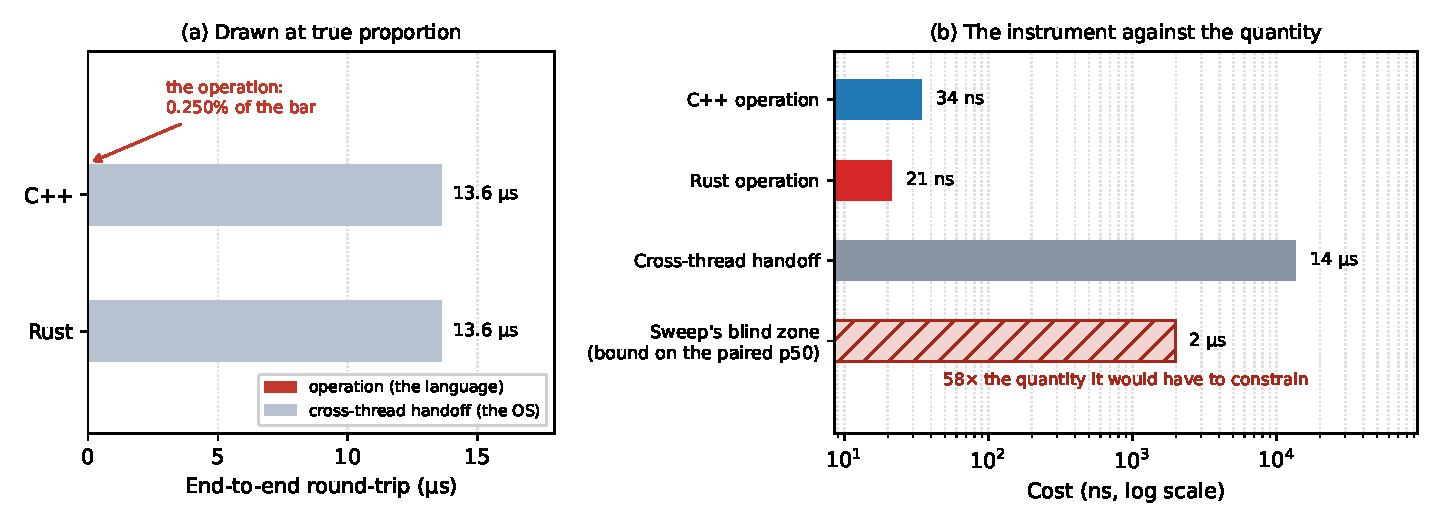
\includegraphics[width=0.78\linewidth]{figures/fig_budget.pdf}
\caption[The end-to-end operation decomposed, against what the sweep can resolve]{Where an end-to-end operation's cost goes, and why the sweep cannot bound a language
effect. \textbf{(a)} The round-trip at true proportion: the operation the language performs is
$\BudgetCoreShareMax\%$ of the bar, the remainder the cross-thread handoff. \textbf{(b)} The
same quantities on a log axis against the smallest paired difference the sweep can resolve,
shown as a blind zone. Both operation measurements fall inside it by a factor of
$\BudgetBoundVsCore$, which is why the differences the sweep does resolve in time are differences
in the round-trip and not in the work the language
performs.\label{fig:budget}}
\end{figure}

The attribution needs care, because the obvious reading is the wrong one. Nothing here implicates
the borrow checker, bounds checking or ownership. The candidate is already recorded in the
forced divergences. The per-shard container is each language's standard hash map, and those are
different data structures. C++'s \texttt{std::unordered\_map} has to be node-based to keep its
iterator- and reference-stability guarantees, so a lookup chases a pointer out of the bucket
array into a separately allocated node. Rust's \texttt{HashMap} is an open-addressed table that
keeps entries inline and usually resolves a lookup within one cache line. The hash function is
pinned to FNV-1a on both sides precisely so that hashing could not be the explanation. That is a
real and reportable difference between the two languages as they are actually used, because a
developer reaching for the standard hash map gets whichever one their language ships. It is not
evidence about Rust's safety model. A second bare-metal campaign replaces the structural argument with a measurement, and its
counters qualify it: the Rust build retires fewer instructions in fewer cycles while missing cache
more often per thousand instructions, so what they support is less work per operation rather than
the better locality this paragraph would predict. Two limits keep the finding the size it is. It
is a single-threaded, uncontended microbenchmark, so it says what the operation costs and not what
a loaded system does with it, and it is one operation on one data structure. Generalising from it
to ``Rust is $\BudgetCoreRatio\times$ faster'' would repeat the error this thesis criticises in
the average-case literature.

\paragraph{Latency, throughput and the knee across the sweep.}
Figure~\ref{fig:loadsweep}(a) plots p99 latency against offered load, and the shape is the
saturation cliff Section~\ref{sec:uecm} described, with one feature sharper. Through the whole
tracking region p99 is \emph{flat}: $\PNineNineLightest\,\mu$s at the lightest load and
$\PNineNineTrackingTop\,\mu$s at the top of the region, a drift of
$\PNineNineTrackingDrift\,\mu$s across a fifty-fold increase in offered load. A queueing model
would predict a gentle climb, and there is none to see, because until a worker saturates its shard
the queue never holds more than a request or two and latency is service time and not waiting
time. Then, in the single step of the rate ladder that follows, p99 rises by four orders of
magnitude, from $\PNineNineTrackingTop\,\mu$s to seconds. That is the overload cliff, and how abruptly it arrives is the finding. One increment of
offered load separates a service meeting millisecond deadlines from one missing them by three
orders of magnitude. A design with bounded blocking queues has no graceful degradation to offer
in between. The flatness before the cliff is why: no rising-latency region warns an operator that
capacity is close. Section~\ref{sec:statsbrief} tests no percentile past the knee, for two
reasons. Latency there is accumulated schedule backlog and not service time. The measured phase
is cut off at a fixed width, so every reported percentile above the knee is a lower bound. What
stays interpretable is how much work each variant still completes (Section~\ref{sec:overload}).

Panel~(b) shows achieved throughput against the same axis, and it is the more informative of the
two, because an average over a whole run is far less sensitive than a percentile to interference
landing on individual operations. All four variants track the ideal offered-equals-achieved line
up to an offered $\TrackingLoad$~kops/s, and the lowest plateau any of them reaches is
$\SatKnee$~kops/s. Each knee is bracketed by the rate ladder, not pinned by it, since the
next rung is where an arm stops tracking. Achieved throughput matches offered load below the knee
to within $\ReprLoadShortfall\%$, so the operating point of Table~\ref{tab:latency} is a genuinely
\emph{sustained} load and its latencies are not those of an already-queueing system.

The knee does \emph{not} sit at the same place for all four variants, which the identical
thread-per-shard structure predicts that it should. The two C++ arms stop meeting their offered
rate after $\TrackingLoadCpp$~kops/s and the two Rust arms carry one rung further, to
$\TrackingLoadRust$, a separation by language and not by allocator as it is everywhere else in
this regime. At the rung between the two limits, $\KneeGapLoad$~kops/s, the consequence is the
largest throughput gap anywhere in the sweep: \KneeGapFaster{} still serves
$\KneeGapThrFast$~kops/s while \KneeGapSlower{} has collapsed to $\KneeGapThrSlow$, a factor of
$\KneeGapRatio$, in \KneeGapAgree{} paired repeats. What that rung licenses is bounded. It is \emph{not} added to the tested family of
Section~\ref{sec:statsbrief}, because the operating point was identified after seeing the sweep.
The family is fixed in advance precisely so that a point chosen that way cannot enter it,
whatever its $p$-value would be. It is reported descriptively instead, with its per-repeat
agreement, and the tested comparison remains the pre-committed overload point of
Section~\ref{sec:overload}. One rung of a geometric ladder is also coarse. The true C++ limit
lies between $\TrackingLoadCpp$ and $\KneeGapLoad$~kops/s, so the difference in \emph{capacity}
is bounded by the ladder's spacing and not measured to better than that. And the direction here
is the opposite of the direction deeper into overload, where C++ sustains more
(Section~\ref{sec:overload}). Both are real, they belong to different loads, and neither cancels
the other.

\begin{figure}[ht]
\centering
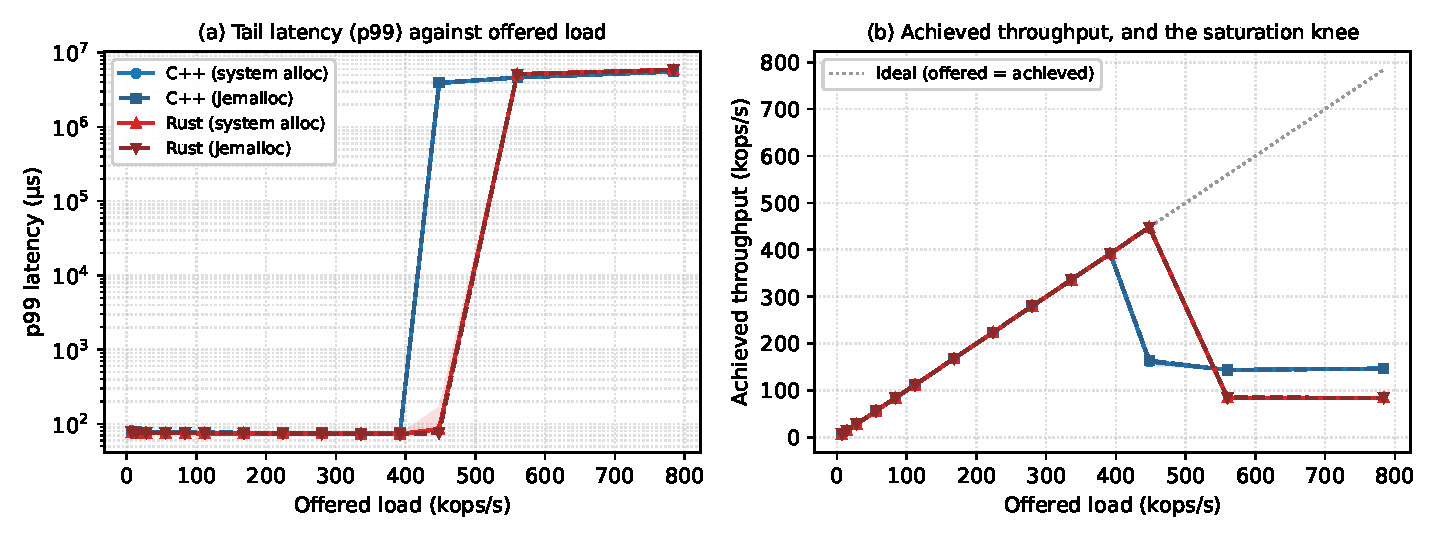
\includegraphics[width=0.78\linewidth]{figures/fig_load_sweep.pdf}
\caption[The load sweep: tail latency and achieved throughput]{The load sweep, both panels
against offered load. \textbf{(a)} Tail latency (p99) for the four build variants on a log axis,
flat across the whole tracking region and then rising by four orders of magnitude in one step of
the ladder. \textbf{(b)} Achieved throughput, with the dotted line marking the ideal
offered-equals-achieved regime. The C++ curves leave that line after an offered
$\TrackingLoadCpp$~kops/s and the Rust curves after $\TrackingLoadRust$, so
$\KneeGapLoad$~kops/s is the only load in the sweep at which the two languages differ in
\emph{throughput} with Rust ahead. Lines are medians over \NRepeats{} repeats and shaded bands are
bootstrap $95\%$ confidence intervals in both panels, which share the variant styling of the
legend in (a). Throughput is counted over the measured phase only.\label{fig:loadsweep}}
\end{figure}

Figure~\ref{fig:tailpct} holds the load fixed instead and sweeps the percentile. The four variants
are close at the median and fan out as the percentile rises, the expected shape for a heavy-tailed
distribution and the reason a percentile-aware methodology is used throughout, and here the fan
opens by language: the two Rust curves stay below the two C++ curves across the whole range, with
the gap widening. Whether that is a language effect or a measurement artefact is what the
right-hand panel is built to answer, and on this host the answer is the first. It sets the spread
between the four variants against the widest interval on any one of them, and the interval stays
the smaller quantity at every percentile it covers, reaching at most $\TailResolveRatioMax$ times
the spread at \TailResolveRatioMaxAt{}, so the fan marks where the languages differ and not where
the measurement runs out. That panel was added when the answer went the other way and is retained
now that it does not, because a reader has no way to tell a resolved comparison from an unresolved
one unless the study shows the same diagnostic in both cases. It stops at p99.9, since the far
tail is reported pooled and a pooled percentile carries no across-repeat interval to weigh a
spread against.

\begin{figure}[ht]
\centering
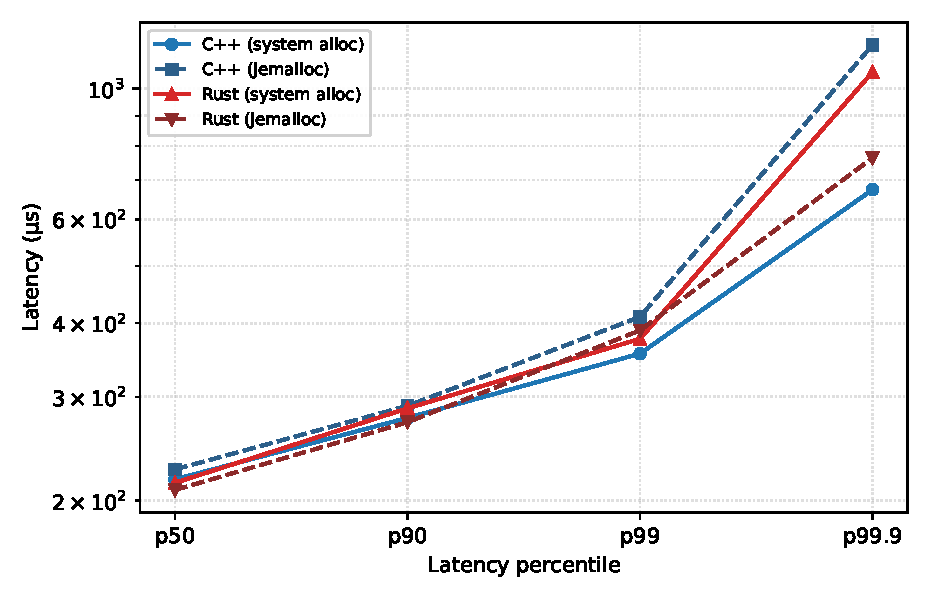
\includegraphics[width=0.78\linewidth]{figures/fig_tail_percentiles.pdf}
\caption[Latency across the percentile range, and how far it resolves]{Per-operation latency
across the percentile range at $\ReprLoad$~kops/s. \textbf{(a)} The four variants as medians over
\NRepeats{} repeats, each with a bootstrap $95\%$ band. The bands are the point: drawn as bare
lines the curves would read as a claim of equivalence, where what the bands show is two languages
separated at every percentile with the gap widening. \textbf{(b)} How far that separation can be
trusted. The spread between the four variants is set against the widest confidence interval on any
one of them, the ratio annotated above each pair of bars. Once it passes one, the uncertainty
about a single variant exceeds the gap between all four and no ordering can be read off. It does
not pass one anywhere here, peaking at $\TailResolveRatioMax$ at \TailResolveRatioMaxAt{}, and on
the virtualised host it passed one above the median. Both panels
stop at p99.9, because both are built from per-run percentiles and the reported p99.99 is pooled
instead, so its ordering in Table~\ref{tab:latency} is licensed by the
millions of operations behind it rather than by this diagnostic.\label{fig:tailpct}}
\end{figure}

\subsection{Past saturation (RQ1)}\label{sec:overload}
RQ1 asks how the two languages compare under increasing load \emph{and overload}, and everything
so far has been below the knee. The operating point here is $\OverloadLoad$~kops/s offered,
defined as the deepest swept load at which every variant has stopped meeting the offered rate.
The metrics are the two that remain interpretable there. Table~\ref{tab:overload} gives what
each variant still sustains and Table~\ref{tab:overloadtest} tests the comparison.

\OverloadSustainedFaster{} sustains $\OverloadThrCpp$~kops/s where \OverloadSustainedSlower{}
sustains $\OverloadThrRust$, a factor of $\OverloadThrRatio$. The paired difference is at least
$\OverloadThrBound$~kops/s under either allocator, it holds in \OverloadThrAgree{} repeats, and
its Holm-adjusted $p$ sits at the corrected floor of the whole family of \NTests{} tests. This is
the largest language effect in the tested family and the most reproducible effect in the study.
One larger ratio appears in the sweep, at the rung between the two languages' saturation limits
(Section~\ref{sec:perfresults}), and it runs the other way and is not tested.

The CPU column rules out the natural reading, that a variant completing less work is simply doing
less, whether throttled, blocked or idle. \OverloadSustainedSlower{} draws \emph{more} total CPU
than \OverloadSustainedFaster{} here, reproducibly and under both allocators, having flipped the
sign it carried at the representative load in Table~\ref{tab:significance}. Divided through by
the work that completed, its CPU cost per sustained operation is $\OverloadCpuPerOpRatio$ times
the other's, and neither variant is near the capacity of the machine, since both sit near six of
the $\MainPinnedCount$ pinned cores. The gap is therefore neither a capacity limit nor idleness.
It is effort spent without completing operations, which is the signature of a synchronisation
path that spins, or parks and wakes repeatedly, where the other blocks once and sleeps.
Figure~\ref{fig:overload} puts both halves of that reading side by side, and its grouping adds a
third: the separation falls almost entirely inside the allocator groups, so the effect follows the
variable the study manipulates and not the one it controls for.

\begin{figure}[ht]
\centering
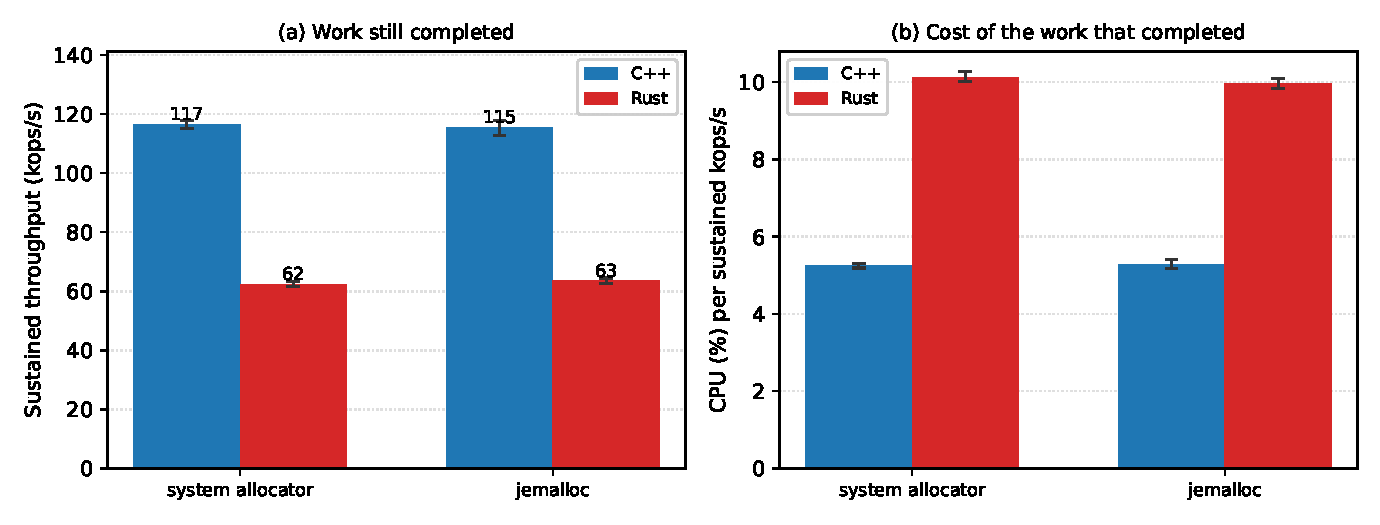
\includegraphics[width=0.78\linewidth]{figures/fig_overload.pdf}
\caption[Divergence past saturation]{Behaviour at $\OverloadLoad$~kops/s offered, well beyond the $\SatKnee$~kops/s knee. Bars
are medians over \NRepeats{} repeats with bootstrap $95\%$ intervals, grouped so that the two
bars inside a group differ only in language. \textbf{(a)} What each variant still completes:
\OverloadSustainedFaster{} sustains a factor of $\OverloadThrRatio$ more than
\OverloadSustainedSlower. \textbf{(b)} Total CPU divided by the work that actually completed,
which is what rules out the reading that the variant delivering less is simply doing less. It
spends $\OverloadCpuPerOpRatio$ times as much CPU per sustained operation, and the CPU figures
are summed across threads.\label{fig:overload}}
\end{figure}

Where that effort goes is narrowed by measurement. Past saturation the producers spend almost all
their time in two places, the bounded blocking queue and the
completion handle, and the microbenchmark below isolates those primitives and does not reproduce
the full-service ordering at significance. That rules them out \emph{alone} as the whole
explanation for a $\OverloadThrRatio\times$ gap. As in Section~\ref{sec:budget}, nothing in the
safety model is implicated. The setting bounds the rest, and Section~\ref{sec:standing} says how
far it travels: the depth of the collapse depends on one design, one request outstanding per
producer and a queue bound of $1\,024$, measured with a harness whose producers block per
request. What travels is the ordering under collapse, and that the isolated primitives do not
produce it on their own. The closest prior work reports a comparable degradation past a threshold
request rate and attributes it to the asynchronous runtime~\cite{arvidsson2025async}.
Section~\ref{sec:rqdiscussion} takes up what it means that the same shape appeared here with no
such runtime on either side.

\begin{table}[H]
\centering
\small
\caption[What each variant sustains past saturation]{What each variant still sustains at
$\OverloadLoad$~kops/s offered, well beyond the $\SatKnee$~kops/s knee: the median over
\NRepeats{} repeats above its bootstrap $95\%$ confidence interval. Below saturation achieved
throughput is pinned to the offered rate by construction and can express nothing about the
languages. Here it is the only thing that can. CPU utilisation exceeds $100\%$ because it is
summed across threads, so $600\%$ is six busy cores of the $\MainPinnedCount$
pinned.\label{tab:overload}}
\begin{tabular}{@{}l r r@{}}
\hline\hline
Variant & sustained throughput (kops/s) & CPU (\%) \\
\hline
C++ (system alloc) & \mci{146.7}{146.3}{147.2} & \mci{662.8}{662.5}{663.6} \\
C++ (jemalloc) & \mci{146.4}{146.1}{146.9} & \mci{664.3}{663.3}{664.9} \\
Rust (system alloc) & \mci{84.5}{84.2}{84.7} & \mci{681.8}{680.4}{682.5} \\
Rust (jemalloc) & \mci{84.3}{83.9}{84.6} & \mci{680.3}{679.8}{681.5}
\\
\hline
\end{tabular}
\end{table}

\begin{table}[H]
\centering
\small
\caption[Exact paired test past saturation]{Exact paired permutation test of C++ against Rust at
$\OverloadLoad$~kops/s, the allocator held fixed, Holm-corrected across the same family of
\NTests{} tests as Table~\ref{tab:significance} rather than as a family of its own. ``Repeats''
counts how many of the \NRepeats{} paired differences agree with the sign of the median, which a
statistic computed from their mean cannot show. No latency percentile is tested here, for the
reason fixed in advance in Section~\ref{sec:statsbrief}.\label{tab:overloadtest}}
% The generated metric names are long enough that six l/r columns overrun the text
% block; the first column wraps instead, and the inter-column padding is tightened.
\setlength{\tabcolsep}{4pt}
\begin{tabular}{@{}p{0.24\linewidth} l r c r r@{}}
\hline\hline
Metric & Allocator & Effect (Rust $-$ C++) & Repeats & $p$ & Holm \\
\hline
Sustained throughput (kops/s) & system & \mci{-62.2}{-62.9}{-61.6} & 20/20 & 0.0000019 & 0.000027 \\
Sustained throughput (kops/s) & jemalloc & \mci{-62.2}{-62.7}{-61.6} & 20/20 & 0.0000019 & 0.000027 \\
CPU utilisation (\%) & system & \mci{+19.5}{+17.3}{+19.9} & 20/20 & 0.0000019 & 0.000027 \\
CPU utilisation (\%) & jemalloc & \mci{+16.8}{+15.6}{+17.5} & 20/20 & 0.0000019 & 0.000027
\\
\hline
\end{tabular}
\end{table}

\paragraph{The contended queue and completion primitives on their own.}\label{sec:contention}
The overload result attributes its gap to the two forced-idiom synchronisation constructs from the
shape of the full-service measurement, so a microbenchmark isolates those constructs alone.
\ContentionProducers{} producer threads hammer one bounded queue of capacity $1\,024$ while a
single consumer drains it, each submitting a no-op job carrying a one-shot completion handle and
blocking until the consumer signals, with no \texttt{ShardCore} work in the path. C++ uses the
hand-written \texttt{BoundedQueue} of Section~\ref{sec:designbrief} with
\texttt{std::promise}/\texttt{std::future}, Rust \texttt{sync\_channel} and a fresh
\texttt{mpsc::channel()} per request. Each timed window lasts two seconds after a warmup, and
\ContentionRepeats{} interleaved repeats are summarised as medians with bootstrap intervals and
tested with the exact paired permutation procedure of Section~\ref{sec:statsbrief}.
Table~\ref{tab:contention} reports the result.

\begin{table}[tp]
\centering
\small
\caption[Throughput through the contended synchronisation primitives alone]{Throughput through
the bounded queue and completion primitives alone, with \ContentionProducers{} contending producers
and queue capacity $1\,024$. Values are medians over \ContentionRepeats{} interleaved repeats above
bootstrap $95\%$ confidence intervals. The paired test compares C++ against Rust on sustained
throughput (kops/s). Like Table~\ref{tab:budget} it predates the move to bare metal and carries no
environment record, so the comparison between the two alternately measured arms is what this section
uses.\label{tab:contention}}
\begin{tabular}{@{}l r r r@{}}
\hline\hline
Language & Throughput (kops/s) & Mean ns/op & Paired $p$ \\
\hline
C++ & \mci{55.0}{53.7}{58.4} & \mci{18178}{17110}{18632} & \multicolumn{1}{c}{---} \\
Rust & \mci{58.7}{56.8}{61.8} & \mci{17045}{16169}{17594} & 0.226
\\
\hline
\end{tabular}
\end{table}

The isolated primitives do not reproduce the overload ordering. C++ sustains
\ContentionThrCpp{}~kops/s and Rust \ContentionThrRust{}~kops/s, a gap of only
$\ContentionRatio\times$ with $p = \ContentionP$. The full service at $\OverloadLoad$~kops/s
separates by $\OverloadThrRatio\times$ with its corrected $p$ at the family floor. The overload
divergence therefore involves extra work the microbenchmark strips away: the larger tagged
\texttt{Request} on the C++ side, the worker's variant dispatch, and the map operations that
still execute in overload. An orders-of-magnitude difference in the primitives alone is ruled
out. That moves the search for the mechanism to the rest of the handoff path and not to the
safety model.

\subsection{Resource use (RQ3)}\label{sec:resources}
Table~\ref{tab:resource} reports resource use at the same sustained load. Peak resident set size
separates the two \emph{languages} cleanly, whichever way the family is read. Its paired intervals
exclude zero, its effect keeps its sign under both allocators, and both rows clear the
correction. It does not separate all four variants, because the C++ build with \texttt{jemalloc}
and the Rust build with the system allocator land on the same footprint from opposite directions.
Figure~\ref{fig:resources} plots the same measurement, and its middle panel is where this
section's finding sits.

Two effects are present in it, not one, and they are of comparable size. Linking \texttt{jemalloc}
costs $\RssAllocDiffLo$--$\RssAllocDiffHi$~MiB in either language. The Rust build costs
$\RssLangDiffLo$--$\RssLangDiffHi$~MiB more than the C++ build under either allocator, with a
bootstrap interval of $\RssLangCILo$ to $\RssLangCIHi$~MiB. Neither dominates. Part of the
allocator figure comes from the fairness controls rather than from \texttt{jemalloc} in general.
Both builds pin the arena count identically, so that neither language's default could become an
accidental advantage, and pinning it high makes the arena metadata a fixed cost on both sides. A
deployment tuning \texttt{jemalloc} for footprint instead of for comparability would not pay it.

The relative size of the two effects is the one result in this chapter that a change of host
overturned. On the virtualised machine the allocator effect measured
$\GuestRssAllocLo$--$\GuestRssAllocHi$~MiB, about $\GuestRssAllocOverLang$ times the language
effect rather than comparable to it, while the language effect was the same size there as here. So the \emph{language} effect on peak RSS is reproducible across
three machines and the \emph{allocator} effect is not a constant of the allocators.

Every row in the upper block of Table~\ref{tab:significance} now clears the correction, including
peak RSS under \texttt{jemalloc}, which did not on the previous host. That row failed there for a
reason in the statistic rather than in the software: a handful of runs reported a resident set some
$\GuestRssLowRunOffset$~MiB low, and a permutation statistic built on a mean of paired differences
is dominated by them. The same measurement here spreads by $\RssLowRunOffset$~MiB, so the
contamination was the machine's. The rule fixed in advance in Section~\ref{sec:statsbrief} for reading
such a row against its interval was not needed, and it stays stated because a design that declares
its reading rules only when they rescue a result is not applying them.

CPU utilisation behaves differently again, by regime rather than by noise. At this
below-saturation operating point Rust draws slightly \emph{less} CPU, by at most
$\CpuDiffAbsMax$ percentage points, consistently under both allocators and clearing the correction
under both, where Section~\ref{sec:overload} finds the sign flipped past saturation and the
magnitude much larger. Achieved throughput adds nothing here, for the reason
Section~\ref{sec:statsbrief} gives: below saturation it is pinned to the offered load, and it is
reported only to confirm that the point is sustained and not merely nominal, which it is to within
$\ReprLoadShortfall\%$.

The memory finding is a difference in fixed cost and not in cost per context. At the $\SweepUes$
active UEs used in the sweep, the $\UeCtxGapBytes$-byte layout difference of
between the two context structures accounts for roughly $\UeCtxGapTotalKB$~kB, two orders of magnitude
short of the gap, so most of it is runtime and allocator-arena overhead, which does not scale with
the workload and would matter proportionally less in a larger deployment. That is an argument from
elimination and this campaign cannot do better, because it reads the resident set only through
\texttt{getrusage}. A second bare-metal campaign reads the allocator's own accounting on a host
that also exposes hardware counters and decomposes the same gap directly
(Table~\ref{tab:resident}). The RQ3 finding is
therefore neither the flat ``no resource penalty'' that overlapping intervals would suggest nor a
general one. Rust costs a few megabytes more of fixed footprint under both allocators, comparable
to what the allocator choice costs here though not on every host measured, and its CPU cost
changes sign with the load regime.

\begin{table}[H]
\centering
\small
\caption[Resource use at the representative load]{Resource use at a sustained offered load of $\ReprLoad$~kops/s: achieved throughput,
peak RSS, and total CPU utilisation. The median over \NRepeats{} repeats above its bootstrap
$95\%$ confidence interval. CPU separates the two languages outright. Peak RSS separates them at a
fixed allocator, which is the comparison the paired test makes, and not across all four variants,
because the allocator effect and the language effect are of comparable size and one middle pair
therefore coincides.\label{tab:resource}}
\begin{tabular}{@{}l r r r@{}}
\hline\hline
Variant & throughput (kops/s) & peak RSS (MiB) & CPU (\%) \\
\hline
C++ (system alloc) & \mci{27.99}{27.99}{27.99} & \mci{9.4}{9.4}{9.5} & \mci{66.8}{65.8}{68.2} \\
C++ (jemalloc) & \mci{27.95}{27.95}{27.96} & \mci{65.9}{65.9}{65.9} & \mci{64.6}{63.4}{66.1} \\
Rust (system alloc) & \mci{27.99}{27.99}{27.99} & \mci{11.2}{11.1}{11.3} & \mci{63.3}{62.2}{66.0} \\
Rust (jemalloc) & \mci{27.95}{27.92}{27.96} & \mci{67.2}{65.4}{67.3} & \mci{63.0}{62.4}{64.5}
\\
\hline
\end{tabular}
\end{table}

\begin{figure}[ht]
\centering
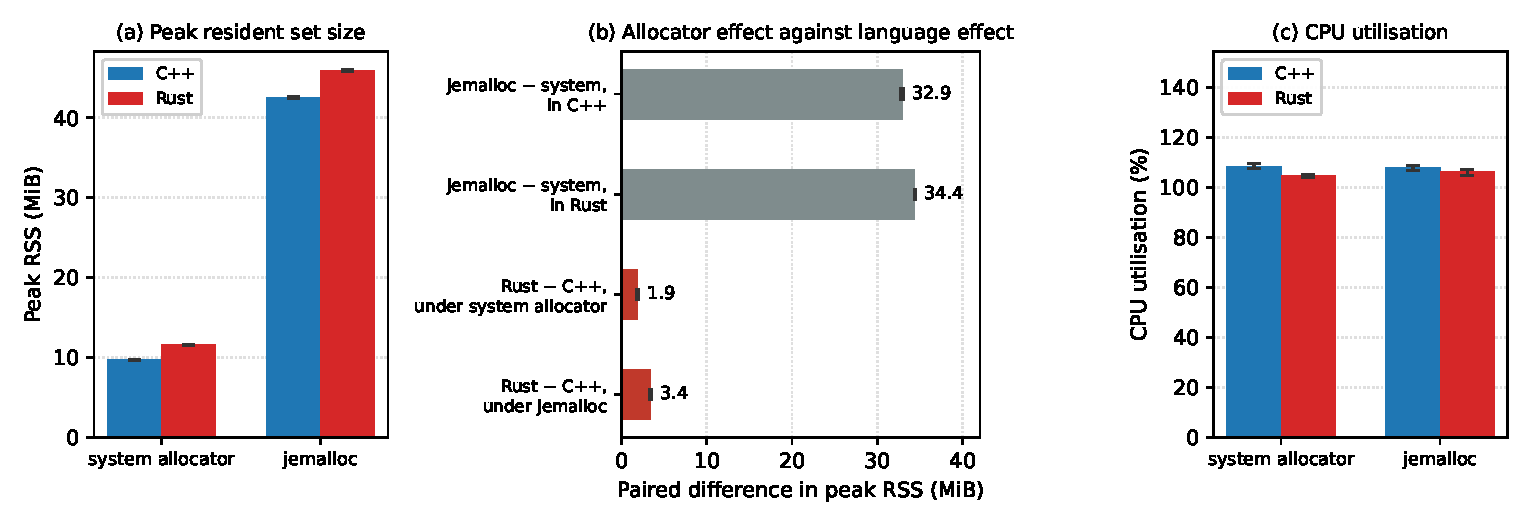
\includegraphics[width=0.78\linewidth]{figures/fig_resources.pdf}
\caption[Resource use, and the two effects inside peak RSS]{Resource use at a sustained offered load of $\ReprLoad$~kops/s, grouped by allocator so
that the two bars in a group differ only in language and the two groups differ only in allocator.
Medians over \NRepeats{} repeats with bootstrap $95\%$ intervals. \textbf{(a)} Peak resident set
size. \textbf{(b)} The two effects it contains, each as a paired difference over the same
repeats: linking \texttt{jemalloc} costs $\RssAllocDiffLo$--$\RssAllocDiffHi$~MiB, while the Rust
build costs $\RssLangDiffLo$--$\RssLangDiffHi$~MiB more than the C++ one. Both are real and on a
shared axis they are of comparable size, which was not true on the host this study used first. \textbf{(c)} CPU utilisation, summed across threads, where the
difference runs the other way and is small.\label{fig:resources}}
\end{figure}

Which of these performance and resource findings belong to the code and which belonged to the
machine is a separate question, and one a single-host study cannot ask.
Two further campaigns bear on it, the virtualised host this study measured on first and a second
bare-metal host at another design, and what survived each change is this: the overload divergence
and the peak-RSS language effect did, the ratio between the language and allocator effects did
not, and hardware counters on the second host turn Section~\ref{sec:budget}'s structural argument
into a measurement.

\subsection{Safety via fault injection (RQ2)}\label{sec:safetyresults}
This study does not claim that Rust has no bugs. It injects the catalogue of $\FaultClasses$
defects set out in Section~\ref{sec:uecm}, each as a small self-contained program flavoured
with the subsystem's domain so that it maps onto a plausible bug in the service. The split into
two groups is what the method of Section~\ref{sec:methodbrief} turns on. Seven classes come from
inside the region Rust claims to govern. Seven are chosen precisely because safe Rust is expected
\emph{not} to prevent them. With the second group the study measures a boundary instead of
demonstrating a claim. A case that unexpectedly compiled, or unexpectedly failed to, surfaces
against its recorded expectation instead of being absorbed into the conclusion.

\paragraph{Procedure.}
Each C++ defect is built and run under AddressSanitizer, ThreadSanitizer and
UndefinedBehaviorSanitizer. The matching construct is written in safe Rust and compiled.
Signed overflow is invisible to the first two sanitisers, so without its own column the
integer-overflow class would be recorded as undetected in C++ when in fact it is caught. No
static analyser is run, so the C++ columns of Table~\ref{tab:taxonomy} report the tooling this
study ran and not a ceiling. Where the Rust program compiles, it is run under a bounded timeout,
because compiling alone would not establish whether the defect survives.

\paragraph{Results.}
The outcomes are shown in Table~\ref{tab:taxonomy}, measured with \texttt{g++~13.3}
(\texttt{-std=c++23}, \texttt{-O0} so the optimiser cannot elide an injected defect) and
\texttt{rustc~1.97} (edition~2021). That C++ toolchain is the local development machine's and not
the measurement host's \texttt{g++~\MainGpp}, deliberately, because whether a program compiles,
and what a sanitiser reports when it runs, are properties of the toolchain and not of the machine
hosting it.

Every one of the seven memory-safety and data-race defects is a compile error in safe Rust. In
C++ each is valid code whose defect shows up only at runtime, and only if a test exercises the
buggy path. Each sanitiser covers a different part of the catalogue and no single one covers it.
The three between them still leave $\FaultClassesUndetected$ of the $\FaultClasses$ classes
untouched, with a fifth reported only intermittently. The parenthesised codes are the
\texttt{rustc} diagnostics that fire: conflicting mutable borrows (\texttt{E0499}), a mutable
borrow while a shared borrow is live (\texttt{E0502}), use of a moved value (\texttt{E0382}), and
a closure outliving borrowed data as it escapes to another thread (\texttt{E0373}). Two rows carry
more than the other five. The use-after-move is the only in-guarantee class no C++ sanitiser
reports at all: all three tools run clean while the acknowledgement goes out under an empty
identity. A static analyser configured for it would plausibly flag the
pattern, and \texttt{clang-tidy} ships such a check, whose documentation records that it follows
control flow but not paths and considers only local variables and function
parameters~\cite{clangtidyuseaftermove}. None is run here, for the reason given in
Section~\ref{sec:methodbrief}. The thread-unsafe handle's diagnostic is \texttt{E0277}, a trait
bound rather than a borrow error, because the rejection comes from \texttt{Send} and not from the
borrow checker.

All seven boundary cases behave as predicted, and they mark out the edge of the claim. Every one
compiles in safe Rust and every one misbehaves. The lost-update case ends in both languages with
a silently wrong answer: against an expected total of $\LostUpdateExpected$ increments the
safe-Rust program recorded $\LostUpdateRustHandled$ and the C++ program under ThreadSanitizer
$\LostUpdateCppHandled$, losing $\LostUpdateRustLost$ and $\LostUpdateCppLost$. Neither language
is meaningfully better off, which is the point of carrying the class at all. The deadlock hangs
in both, the reference cycle leaks in both, the release-build overflow produces a wrong tunnel
endpoint identifier (TEID) in both, and a failure inside one shard worker takes down more than
that shard in both. The forgotten guard separates two things that resource acquisition is
initialization (RAII) runs together whenever it is credited with preventing this. Rust removes the
ordinary form of the bug, since the C++ version fails on a validation path that returns before a
hand-written unlock and the Rust version has no unlock to skip, but it does not remove the class: both programs had to be killed by the timeout and neither language's
tooling said anything.

The seam double-free is the double-free of the in-guarantee group, written the way a
foreign-function boundary has to write it. Safe Rust rejects the double release with
\texttt{E0382}, and handing a C caller a raw pointer is precisely the operation that ends the
ownership tracking behind it. \texttt{Box::from\_raw} then asserts ownership of whatever address
it is given, so asserting it twice frees the storage twice. The C++ half of the pair is
deliberately unremarkable and unchanged, so the only column that moves is the Rust one, and that
boundary is the one Section~\ref{sec:migrationresults} measures.

Two of the seven are cases where the C++ tooling is \emph{ahead}. LeakSanitizer reports the C++
reference cycle as an unreachable allocation at exit, while the safe-Rust cycle leaks in silence,
because leaking is safe in Rust by explicit design~\cite{hughes2025gcrust,cui2024rcanary}. UBSan
reports the C++ overflow, because signed overflow is undefined there, while the Rust overflow
wraps by definition at \texttt{opt-level~=~2}. Defined-but-wrong is
easier to debug than undefined-and-wrong and no less incorrect~\cite{dietz2015overflow}.
ThreadSanitizer does flag the inversion in C++, but on some runs and not others,
$\DeadlockTsanHits$ of $\DeadlockTsanRuns$ repeats in the run behind this table while the program
deadlocks on every one, and the rate itself is not stable across runs. TSan builds its lock-order
graph from acquisitions that \emph{succeed}, so the cycle closes only when some thread completes
an inversion without blocking. A positive control that inverts the same two locks without ever
blocking is reported every time, which establishes that the detector was live.

The scope all of this exposes is precise. Rust's concurrency guarantee is the absence of
\emph{data races}. It is not a guarantee about lock-acquisition order, nor about the atomicity of a
composed operation, nor about leaks, wrapping arithmetic, or fault containment, and it is
suspended wherever a program writes \texttt{unsafe}. The lost update stays the quietest case,
because no sanitiser reports it either.

\paragraph{Where the boundary classes are caught, and at what cost.}
RQ2 asks which defects are prevented, and also at what stage the rest are detected. For
the boundary group the sanitiser columns leave that second half largely blank. Two Rust model
checkers answer it, in the division of labour a production Rust system has been validated
with: Loom explores interleavings soundly under bounded partial-order reduction, and Shuttle
samples them probabilistically to reach cases beyond Loom~\cite{bornholt2021shardstore}. Both
report both of the original boundary defects, the deadlock as a closed cycle and the lost update
as a failed assertion. Each is paired with a control in which the defect is fixed, by consistent
lock order and by holding the read-modify-write in one critical section, and both controls come
out clean, so the reports come from the defects and not from the tools.

The cost is the part worth recording. Neither defect program runs under either checker as
written. Each had to be re-imported against the checker's own synchronisation and thread types,
because a tool that does not intercept the primitive cannot schedule it, and each had to be
shrunk to model size: the lost-update model drops from twenty thousand iterations per thread to
one, and the deadlock model loses the sleep that widens its window on real hardware. The answer
for the Rust half of the boundary is therefore \emph{detected at test time, after a rewrite},
while on the C++ half the sanitiser takes the program unchanged and finds one of the two
unreliably and the other not at all. Neither language's story here is the simple one, and
Chapter~\ref{chapter:discussion} develops the consequence for practice.

The seam double-free is answered by a different tool and comes with a sharper limit. Miri
interprets the program and reports the second
release precisely, as a dangling box reconstructed from a freed allocation, while a control that
releases the same handle once is clean, so the stage for this class is test time again and this
time without a rewrite. The limit is what a migration has to weigh. Miri interprets Rust and
cannot execute a C++ host, so the program it checked uses a Rust stand-in for the host. The tool
that finds this defect cannot be pointed at the configuration the defect ships in, which is a
seam with C++ on the other side of it. No shipped tool checks that boundary, and the published
attempt that drives Miri with an interpreter for the foreign side found 46 instances of
undefined or undesired behaviour in 37 libraries that call foreign
functions~\cite{mccormack2025ffi}. That leaves the practical answer
Section~\ref{sec:migrationresults} argues from the prototype: keep
the seam small enough to review by hand, because review is what is left.

\paragraph{A defect that was not injected.}
Every outcome above comes from a defect written on purpose, and that is the standing weakness of
the method. Whoever assembles a catalogue already knows what safe Rust prevents. One case in
this study does not carry that weakness. A design review of the specification found that its
concurrency section forbade submitting an operation outside the service's running window
(before \texttt{start()}, or after \texttt{shutdown()}), while neither implementation checked
for it. The prohibition was addressed to the caller with no mechanism behind it, and in that gap
the two languages did not fail alike. The C++ submit path indexes the shard vector that
\texttt{shutdown()} has cleared, which AddressSanitizer reports as a heap-use-after-free. Called
before \texttt{start()} it is a segmentation fault on the zero page. In Rust both calls were
already a panic, from the ordinary bounds check on the same indexing operation, and nobody had
designed for it.

What makes the case evidentially different is where it came from, not how severe it is. It sat in
code written to be correct, in the arm whose safety claim rests on ThreadSanitizer, reachable
through the public API by calling documented operations in a documented order, and it survived
every check this study runs: $\CppTestBinaries$ C++ test binaries, $\RustTests$ Rust tests,
$\ConfHandOps$ hand-written and $\ConfGenOps$ generated conformance operations, and three
sanitiser configurations reported clean. It survived them because none of them ever called an
operation outside the running window. ASan finds this defect only once a test drives it, which is
the property the cost argument above assigns to runtime detection, seen here on the study's own
artefact instead of a planted one.

The direction in which it must \emph{not} be over-read is the flattering one. Rust did not
prevent this at compile time, and nothing in the borrow checker knows that a service must be
started before it is used. What turned undefined behaviour into a diagnosable failure was a
slice bounds check, a runtime guarantee and so the same kind of assurance the C++ sanitiser
offers, not the compile-time kind Table~\ref{tab:taxonomy} records. The honest claim is that
checking by default turned a specification gap into a panic, not that a type system caught a
lifecycle error. What remains is a panic naming its cause on every build against a
heap-use-after-free that needs an instrumented binary and a test that thinks to look. Both
implementations now reject the call explicitly, in both directions, and both suites cover it.

\begin{table}[tp]
\centering
\small
\caption[Defect-class taxonomy: measured outcomes]{Defect-class taxonomy: measured outcomes for the injected catalogue. C++ under
\texttt{g++~13.3} with ASan/TSan/UBSan. Rust under \texttt{rustc~1.97}, edition~2021. ``Compile
error'' means the safe-Rust program does not build, so the defect cannot be written. The lower
block is the boundary group: defect classes chosen because safe Rust is \emph{not} expected to
prevent them, and does not. Two of those seven are the ones on which the C++ tooling is ahead.
The body of this table is generated from the fault-injection taxonomy log
(Section~\ref{sec:repro}), so it cannot
disagree with the run that produced it.\label{tab:taxonomy}}
\footnotesize
\setlength{\tabcolsep}{4pt}
\begin{tabular}{@{}l l l l l@{}}
\hline\hline
Defect class & ASan & TSan & UBSan & Safe-Rust outcome \\
\hline
\rlap{\emph{Within the guarantee}} & & & & \\
Use-after-free & detected & detected & not detected & compile error (E0499) \\
Double-free & detected & not detected & not detected & compile error (E0382) \\
Iterator invalidation & detected & detected & not detected & compile error (E0502) \\
Data race & not detected & detected & not detected & compile error (E0373$^{\dagger}$) \\
Unguarded shared mutation & not detected & detected & not detected & compile error (E0502$^{\dagger}$) \\
Use-after-move & not detected & not detected & not detected & compile error (E0382) \\
Thread-unsafe handle shared & not detected & detected & not detected & compile error (E0277)\\
\hline
\rlap{\emph{Outside the guarantee}} & & & & \\
Lock-order deadlock$^{\ddagger}$ & not detected & intermittent$^{\S}$ & not detected & compiles, deadlocks \\
Lost update & not detected & not detected & not detected & compiles, wrong result \\
Reference-cycle leak & detected & not detected & not detected & compiles, leaks \\
Integer overflow (release) & not detected & not detected & detected & compiles, wrong result \\
Worker-failure blast radius & not detected & not detected & not detected & compiles, shard outage \\
Double-free in unsafe & detected & not detected & not detected & compiles, aborts \\
Forgotten lock guard$^{\ddagger}$ & not detected & not detected & not detected & compiles, deadlocks
\\
\hline
\end{tabular}

\vspace{0.4em}
{\footnotesize\raggedright
$^{\dagger}$ Several diagnostics fire for these cases. The first is shown (the data race also
raises \texttt{E0382} and \texttt{E0502}, the unguarded mutation \texttt{E0524} and
\texttt{E0597}). \quad
$^{\ddagger}$ On these rows the instrumented binary was killed by the harness timeout rather
than reporting anything. Nothing is corrupted and nothing is undefined, so the tools that
detect corruption have nothing to say. The forgotten guard is silent under all three, and the
lock-order case is the one TSan sometimes catches, as the next note records. \quad
$^{\S}$ ThreadSanitizer reports the lock-order inversion on some runs and not others, measured at
$\DeadlockTsanHits$ of $\DeadlockTsanRuns$ repeats, while the program deadlocks on
every one. The detector builds its lock-order graph from acquisitions that \emph{succeed}, so a
run whose first inversion blocks never completes the second edge of the cycle.\par}
\end{table}

Figure~\ref{fig:taxonomy} draws the same $\FaultClasses$ outcomes as a matrix, where the change
of character at the boundary rule is the shape of the picture and not something to be read off
row by row. Both it and Table~\ref{tab:taxonomy} are generated from the fault-injection taxonomy
log of Section~\ref{sec:repro}, so neither can drift from the other.

\begin{figure}[ht]
\centering
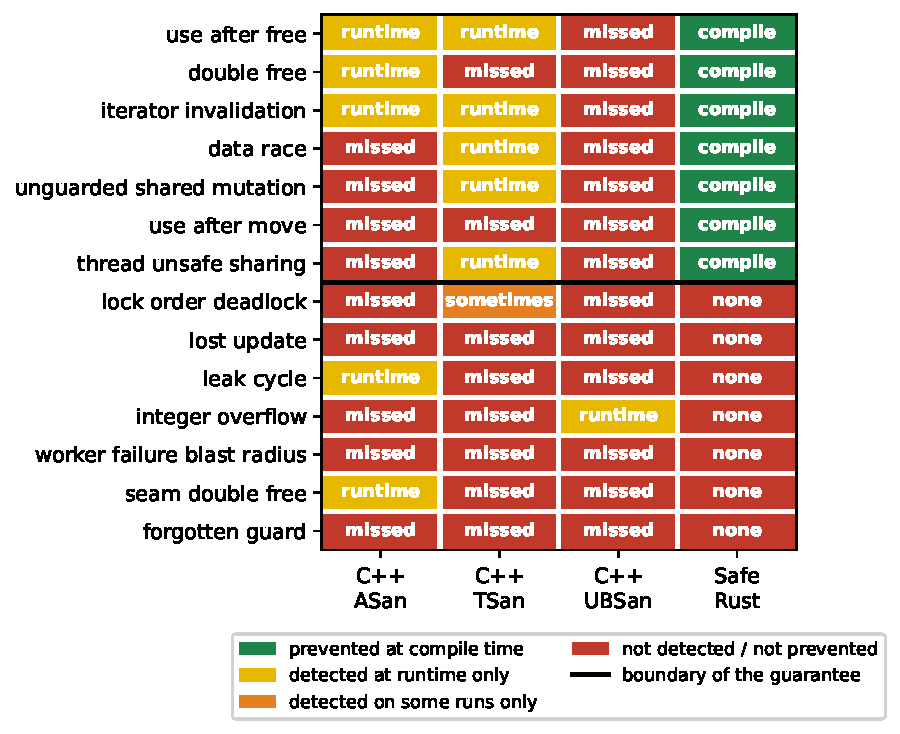
\includegraphics[width=0.72\linewidth]{figures/fig_taxonomy.pdf}
\caption[Where the guarantee stops: the outcome matrix]{The outcomes of Table~\ref{tab:taxonomy} drawn as a matrix, generated from the same
taxonomy log (Section~\ref{sec:repro}). Above the rule the Rust column is a single colour: every
defect is a compile error, so none can be written. The C++ columns there are a patchwork instead,
and no one sanitiser covers them. The use-after-move row is the one no sanitiser covers at all.
Below the rule the Rust column joins them, and on the
reference-cycle leak and the release-build overflow the C++ tooling is ahead. The lock-order
deadlock is the one cell where a tool reports intermittently: ThreadSanitizer flags the inversion
in $\DeadlockTsanHits$ of $\DeadlockTsanRuns$ runs while the program deadlocks on every
one.\label{fig:taxonomy}}
\end{figure}

\subsection{Migration (RQ4)}\label{sec:migrationresults}
Incremental adoption is assessed with a working prototype, built in the direction a real
migration takes. An existing C++ host keeps a Rust component behind a C ABI. The Rust service is
exposed through a thin \texttt{extern "C"} seam in a \emph{separate} crate that depends on the
unmodified core library, so adopting the component needs no change to the component itself. The
C++ host sees only an opaque handle and a set of plain-C entry points (a hand-written header, no
generated bindings). It drives the full UE lifecycle across the boundary. The error model
crosses intact, so a duplicate connection setup returns \texttt{InvalidState} through the seam.
Figure~\ref{fig:ffiseam} shows the resulting structure and where the \texttt{unsafe} sits.

\begin{figure}[ht]
\centering
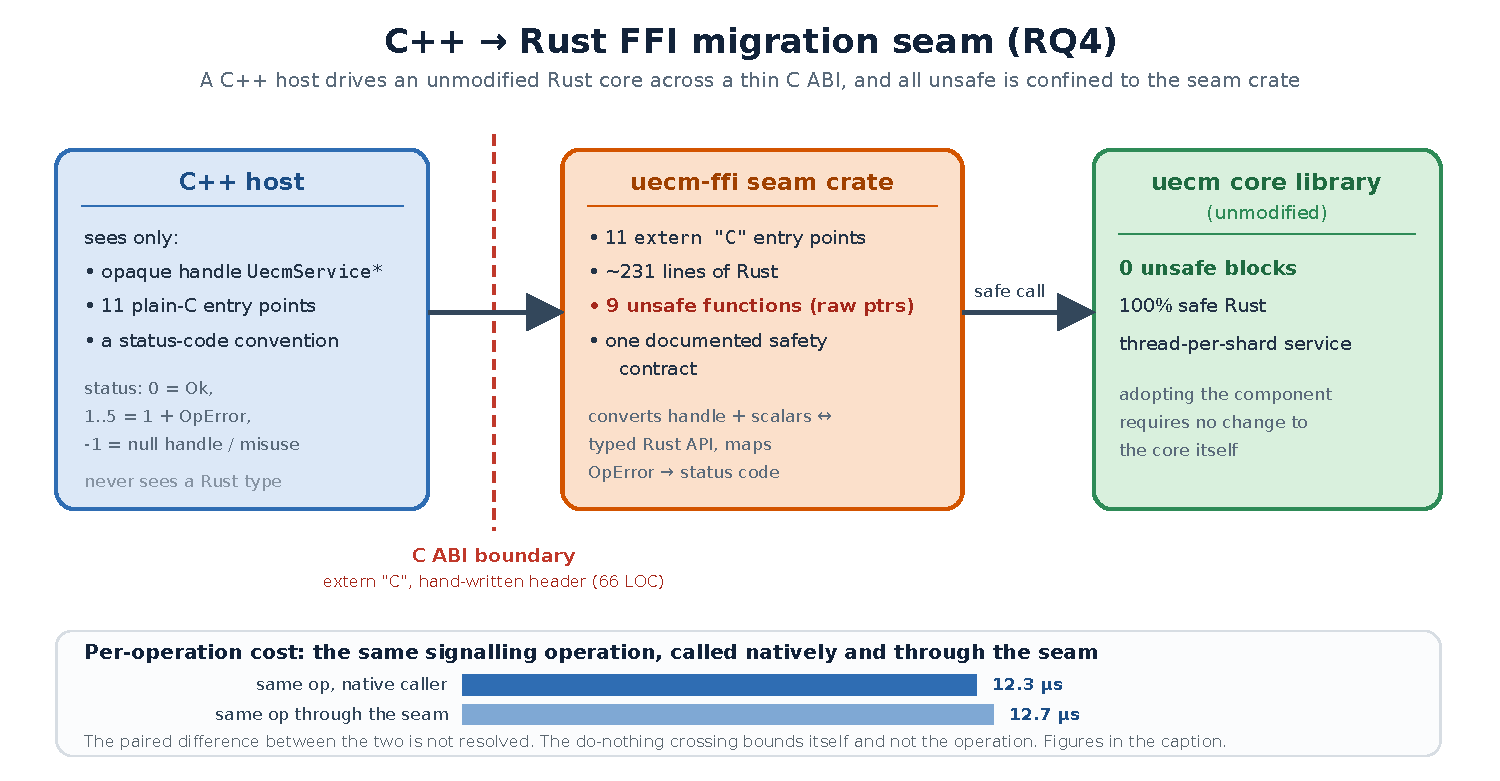
\includegraphics[width=0.78\linewidth]{diagrams/pdf/07_ffi_seam.pdf}
\caption[The C++-to-Rust FFI migration seam]{The C++-to-Rust FFI migration seam. The C++ host sees only an opaque handle, $\FfiEntryPoints$
plain-C entry points, and a status-code convention. A thin \texttt{extern "C"} seam crate
concentrates all of the raw-pointer \texttt{unsafe} ($\FfiUnsafeFns$ functions) and calls the unmodified Rust
core, which remains free of \texttt{unsafe}. The band along the bottom is the comparison the
argument rests on: the same signalling operation called natively at $\FfiOpNative$~\textmu s and
through the seam at $\FfiOpSeam$~\textmu s, whose paired difference is not resolved and is bounded
at $\FfiOpBoundPct\%$ of one operation. The two bars are meant to look alike. The do-nothing
crossing costs $\FfiCrossing$~ns and bounds only itself.\label{fig:ffiseam}}
\end{figure}

Table~\ref{tab:ffi} summarises the interop cost. The seam is small, $\FfiEntryPoints$ C-ABI entry
points in $\FfiSeamLines$ lines of Rust plus a $\FfiHeaderLines$-line C header with no third-party
FFI dependency, and its safety boundary is clean: the core library stays free of \texttt{unsafe}
and the raw-pointer handling the C ABI requires is confined to the seam crate, in its
$\FfiUnsafeFns$ \texttt{unsafe} functions, under a single documented safety contract. The C++ side
never sees a Rust type.

\begin{table}[H]
\centering
\caption[FFI migration prototype: seam size, safety, and cost]{FFI migration prototype: seam size, safety boundary, and per-call interop cost
(C++ host calling the Rust component across a C ABI, \texttt{-O2}). The core library is
unmodified and \texttt{unsafe}-free. All interop is confined to the seam crate. The last
three rows are the direct comparison: one signalling operation on the same service
configuration and the same loop, invoked natively and then through the seam, so the
difference isolates what the boundary adds rather than what the operation
costs. Like the other paired experiments it predates the move to bare metal and carries no
environment record, so the bound is a ratio between two alternately measured arms and not a claim
about a host.\label{tab:ffi}}
\begin{tabular}{l r}
\hline\hline
Metric & Value \\
\hline
C-ABI entry points & 12 \\
Seam size (Rust \texttt{lib.rs}) & 231 LOC \\
Hand-written C header & 66 LOC \\
\texttt{unsafe} in core library & 0 \\
\texttt{unsafe} in FFI seam & 12 \\
Raw FFI crossing & 2.54 ns/call \\
Signaling op, native caller & 12.3 \textmu s/call \\
Signaling op, through the seam & 12.7 \textmu s/call \\
Seam cost per operation (paired) & $+192$ ns $[-954, +1341]$ \\
\quad as a fraction of the operation & $+10.91\%$ at the upper bound
\\
\hline
\end{tabular}
\end{table}

The per-call cost is measured twice, and only the second measurement answers RQ4's question. The
first is the crossing itself. A do-nothing \texttt{extern "C"} call costs $\FfiCrossing$~ns, an
ordinary indirect call, negligible next to the microsecond-scale round-trip of a signalling
operation. That bounds the crossing and says nothing about what the seam does to a real
operation, whose round-trip is dominated by a cross-thread handoff. An argument that the handoff
``would be paid identically anyway'' is reasoning standing in for a measurement.

The measurement is therefore made directly. The same signalling operation, on the same service
configuration and in the same loop, is invoked natively from Rust and then from C++ through the
seam, interleaved over \FfiOpRepeats{} repeats so the pair is matched. The paired difference is
$\FfiOpDelta$~ns per operation, with a bootstrap interval of $[\FfiOpDeltaLo, \FfiOpDeltaHi]$~ns
and an exact paired $p$ of $\FfiOpP$. No cost is detected, and more usefully the interval bounds
any cost the measurement could have missed at $\FfiOpBoundPct\%$ of the operation. The
interleaving is not optional here. A single pass of each, run while preparing this section, made
the seam look \emph{faster} than calling natively by a third, because the run-to-run spread of the
handoff on a shared host is far wider than anything a C ABI could contribute.
Figure~\ref{fig:fficost} shows the repeats behind those numbers, and its left panel is that
spread: the pairs cross, over a range an order of magnitude wider than the difference under test.

\begin{figure}[ht]
\centering
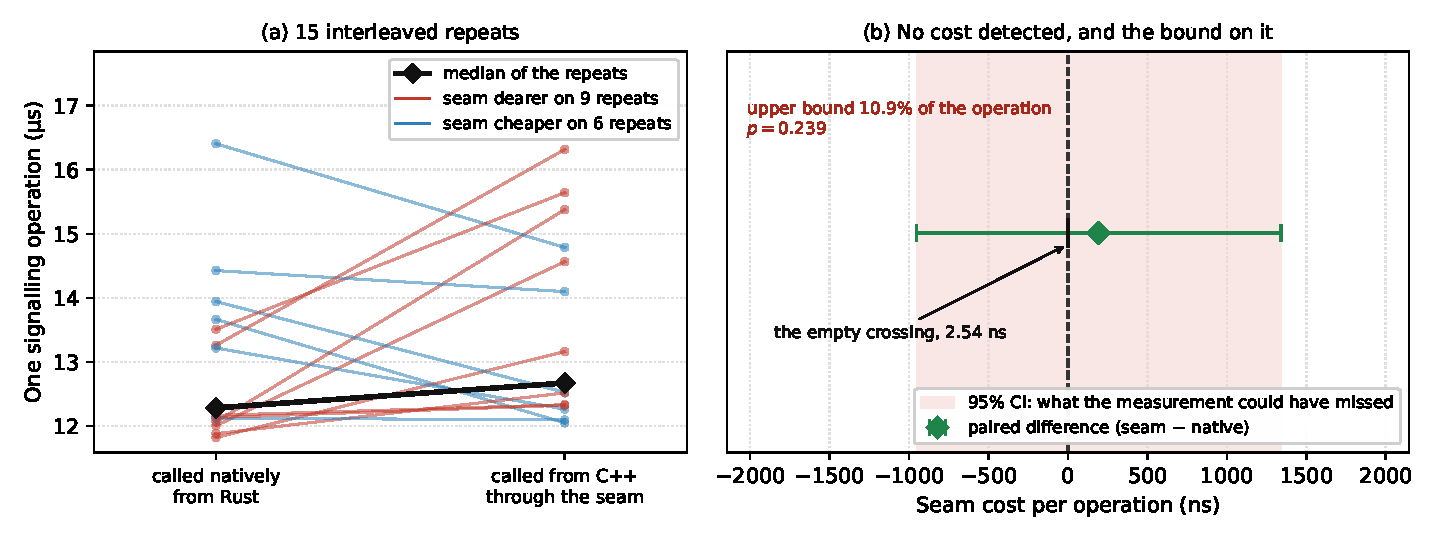
\includegraphics[width=0.78\linewidth]{figures/fig_ffi_cost.pdf}
\caption[The seam's cost on one operation, against its own uncertainty]{The interoperability cost measured on a real operation rather than inferred from an empty
call. \textbf{(a)} The same signalling operation invoked natively from Rust and from C++ through
the seam, one line per interleaved repeat, with the medians in black. \textbf{(b)} The pairs
reduced to their difference: $\FfiOpDelta$~ns per operation with a bootstrap $95\%$ interval of
$[\FfiOpDeltaLo, \FfiOpDeltaHi]$~ns and an exact paired $p$ of $\FfiOpP$. No cost is detected, and
the upper end of that interval is what bounds the cost the measurement could have missed at
$\FfiOpBoundPct\%$ of the operation. The empty \texttt{extern "C"} crossing, $\FfiCrossing$~ns, is
marked for scale rather than as the answer: it is indistinguishable from zero on the axis the
operation is measured on.\label{fig:fficost}}
\end{figure}

The main engineering effort therefore goes into \emph{designing} a C-compatible API surface, with
an opaque handle, scalar-typed operations and a status convention, and not into runtime overhead.
The reverse direction (Rust calling into C++) is symmetric, but it needs a C-ABI wrapper on the
C++ side and it brings \texttt{unsafe} back to the Rust caller. The prototype and its measurements
inform the migration guidelines of Chapter~\ref{chapter:discussion}.

RQ4 asks what adoption costs in effort, interoperability and risk, and the seam answers only the
middle term. Three further axes a team asks about first were measured, and
each complicates a folk version of the answer. Build time survives the objection only in the
aggregate: the full Rust build costs $\BuildAllCpuRatio$ times the CPU \texttt{g++} needs, but
$\BuildDepShareCpu\%$ of that is third-party code and the project's own source compiles in
$\BuildAllFirstPartyCpuRatio$ times what \texttt{g++} spends on its equivalent. The shipped
footprint ordering reverses once the linkage policy is held fixed instead of left at each
toolchain's default. And the compared component resolves $\DepsCore$ crates with $\CoreUnsafe$
\texttt{unsafe} sites, so the transitive-dependency objection does not reach the artefact that
would ship. Build time is the one axis whose absolutes belong to the measuring machine, which is
why it is reported as a paired ratio between two toolchains timed alternately.

\chapter{Discussion\label{chapter:discussion}}

\section{Summary of findings}
Table~\ref{tab:findings} collects the headline finding for each research question with the
strength of the current evidence. The safety results (RQ2) do not depend on the measurement
environment. The migration results (RQ4) depend on it along one axis only, which is why build
time is reported as a paired ratio. The performance and resource results do depend on the host.
They now resolve on the host of Section~\ref{sec:testbed}, including the far tail below
saturation, which the same design on the earlier host could not resolve.

\begin{table}[tp]
\centering
\caption[Summary of findings per research question]{Summary of findings per research question and the current strength of evidence.
\label{tab:findings}}
\renewcommand{\arraystretch}{1.25}
\begin{tabular}{@{}p{0.06\linewidth} p{0.62\linewidth} p{0.22\linewidth}@{}}
\hline\hline
RQ & Headline finding & Evidence status \\
\hline
RQ1 & The answer divides at saturation. Below it the variants agree to $\PFiftyRange\,\mu$s
($\PFiftySpread\%$) at the median, and the far tail resolves in \FarTailLower{}'s favour, the
pooled p99.99 of the two \FarTailLower{} variants sitting below both of the others by up to
$\FarTailRange\,\mu$s. The end-to-end number is only $\BudgetCoreShareMax\%$ operation, so it
cannot bound a language effect in any case, while the operation measured apart is
$\BudgetCoreRatio\times$ faster in \BudgetCoreFaster. Past saturation they diverge decisively and
in both directions: the Rust arms hold their offered rate one rung further, to
$\TrackingLoadRust$~kops/s against $\TrackingLoadCpp$, while at $\OverloadLoad$~kops/s, where all
four have collapsed, \OverloadSustainedFaster{} sustains $\OverloadThrRatio\times$ the throughput
of \OverloadSustainedSlower{} in \OverloadThrAgree{} repeats under both allocators. & Overload,
operation and far tail: resolved, and each reproduced at a second shard count.
Mechanism: tested. Primitives alone insufficient. The saturation-limit gap is descriptive, not
tested \\
RQ2 & All seven injected memory-safety and data-race classes are prevented at compile time in
safe Rust, where in C++ each compiles and is caught, if at all, only at runtime and by no single
sanitiser. The guarantee stops there: the seven boundary classes compile in both languages, and
on the leak and the release-build overflow the C++ tooling reports what Rust's does not. &
Final \\
RQ3 & A memory penalty that reproduces: $\RssLangDiffLo$--$\RssLangDiffHi$~MiB more peak RSS in
the Rust build under \emph{both} allocators, in the same direction and order of magnitude on all
three machines measured. The allocator's own $\RssAllocDiffLo$--$\RssAllocDiffHi$~MiB is
comparable here and was an order of magnitude larger on the virtualised host, so their ratio does
not travel. CPU inverts across the regimes: at the representative
load Rust draws up to $\CpuDiffAbsMax$ percentage points less, and past saturation
$\OverloadCpuPerOpRatio\times$ more per completed operation. & Memory: resolved, and located
outside the allocator by its own accounting. CPU: resolved in both regimes, opposite signs, and
one sign below saturation on the second bare-metal host \\
RQ4 & The seam is small and keeps the core \texttt{unsafe}-free at compile time. Measured against
the same operation called natively, no cost is detected and any tax is bounded at
$\FfiOpBoundPct\%$ of an operation. The real cost is API design. The core remains exposed at run
time to memory errors in the C++ host it shares an address space with. On the adoption axes beyond
the seam, $\BuildDepShareCpu\%$ of the Rust clean build is third-party code and the project's own
code compiles in $\BuildAllFirstPartyCpuRatio$ times the CPU \texttt{g++} needs, the footprint
ordering reverses with the linkage policy, and the compared component resolves $\DepsCore$ crates.
& Final. Build-time absolutes are host-bound, the ratio is not \\
\hline
\end{tabular}
\end{table}

\section{Discussion on the research questions}\label{sec:rqdiscussion}
\paragraph{RQ1 (predictability).} The two load-dependent effects point at opposite languages, so a
single verdict would be false. A service sized to run below its knee should prefer the arm that
holds its offered rate further, to $\TrackingLoadRust$~kops/s against $\TrackingLoadCpp$. One that a signalling storm will drive past every knee should prefer the arm that still
completes more work afterwards, by $\OverloadThrRatio$ at $\OverloadLoad$~kops/s, at the
corrected floor of the whole test family. The slower arm spends more CPU on each operation it
does complete (Section~\ref{sec:overload}). Only the second is tested. The first is descriptive for the reason
Section~\ref{sec:perfresults} gives. A comparison stopping at nominal load, as most in this
literature do, would have concluded the opposite with the same apparatus.

What a deployment sizes its margin from is the far tail. At the representative load the median gap
is a fraction of a $\PFiftyMedian\,\mu$s operation. The pooled p99.99 is an ordering in
\FarTailLower{}'s favour whose extremes differ by $\FarTailRange\,\mu$s, roughly a whole median
operation, reproduced at a second shard count on a second machine. The median result is
consistent with the wider evidence that Rust's safety checks are largely absorbed by modern
out-of-order CPUs~\cite{balasubramanian2017rust,emmerich2019drivers}. It is also weaker than it
looks. The operation the languages execute is $\BudgetCoreShareMax\%$ of what the sweep measures
(Section~\ref{sec:budget}), so an end-to-end comparison in a design dominated by a cross-thread
wakeup describes the design and not the languages. Measured on its own, the operation differs by
$\BudgetCoreRatio\times$.

The overload shape reframes the closest prior work instead of merely agreeing with it. Arvidsson
and Kaller measure this quantity for 5G control-plane procedures and find Rust's 99th percentile
degrading faster beyond a threshold request rate, traced to stackless
\texttt{async}/\texttt{await}, which permits a context switch immediately before an I/O operation
begins~\cite{arvidsson2025async}. Section~\ref{sec:gap} accepts that attribution. This study was
built to exclude the confound behind it: one worker per shard over a bounded blocking queue, and
no asynchronous runtime on either side. Section~\ref{sec:rqs} committed in advance to what each
outcome would mean, and the second branch fired. A degradation past a threshold rate appeared with
the concurrency model held fixed, so the asynchronous runtime cannot be the only place such an
effect starts. The prediction also named where to look first, bounds and overflow
checking~\cite{zhang2022runtime,harris2023morello}, and that part was wrong. The effect appears
only once the handoff path is contended, which points at the two standard libraries' blocking
primitives. Section~\ref{sec:contention} finds that those primitives alone do not reproduce the
full-service ordering at significance. The cause is extra work on the C++ handoff path and not
the safety model.

\paragraph{RQ2 (safety).} The result does not depend on the environment. What makes it interesting
is the half that bounds the expectation and not the half that confirms it. Within its scope the
difference from C++ is one of kind and not of degree. A compiler that refuses to build a program
rules the defect out of every execution. A sanitiser rules it out only of the executions an
instrumented test happens to take. What is absolute is the execution coverage, not the breadth of
the catalogue, which is still the $\FaultClasses$ programs written for it. That fits the Common
Vulnerabilities and Exposures (CVE) evidence that Rust memory-safety bugs always involve
\texttt{unsafe}~\cite{xu2021rustcve} and the caution that unsafety can spread through
dependencies~\cite{evans2020rust}, which is why keeping the core \texttt{unsafe}-free matters. The
seam double-free is that evidence under controlled conditions, the one class safe Rust rejects
and unsafe Rust does not.

The one case reaching past the written programs is the lifecycle defect of
Section~\ref{sec:safetyresults}, found in the implementation rather than written for the
catalogue. It revises the picture in two directions. It strengthens the cost argument, because a
real defect in code written to be correct survived tests, parity vectors and three sanitisers
purely because nothing exercised the path. Runtime detection that depends on test coverage is
weaker in practice than it looks in a table where every row is driven deliberately. It also
narrows what may be credited to Rust, because the contribution was a bounds check and not a
proof. The guarantee worth budgeting for is \emph{checked by default} and not \emph{ruled out
at compile time}. The root cause belongs to the method rather than to either language. A
specification stating a prohibition without assigning a mechanism leaves each implementation to
fail in its own idiom, and the two idioms here are a panic and a use-after-free.

Where the guarantee stops matters just as much to a vendor deciding what Rust buys. The
lock-order deadlock shows that Rust reasons about \emph{aliasing} and not \emph{acquisition
order}. A \texttt{Mutex} guard is an ordinary value whose lifetime the borrow checker tracks
perfectly, and tracking it perfectly says nothing about whether two threads take their locks in
compatible orders. The tooling confirms this is a boundary and not an artefact of the injected
example. Static deadlock detection for Rust is an active research problem~\cite{zhang2026deadlock},
and model checkers for Rust kernel code are motivated explicitly by ownership and borrowing leaving
data races, deadlocks and livelocks reachable~\cite{tang2025converos}. The lost update is
sharper. It escapes ThreadSanitizer for precisely the reason it escapes the borrow checker
(Section~\ref{sec:safetyresults}): with every access correctly synchronised there is no
unsynchronised access to find. Nor is the class marginal. In a field study of $105$ real concurrency bugs, about a third of the non-deadlock cases
violated the order the programmers intended rather than their locking~\cite{lu2008mistakes}.
The authors record that such intentions are not readily expressible through locks at all. The distinction between a data race and a
race condition is the one ``thread safety'' routinely runs together, and Rust removes only the
first.

Adopting Rust therefore retires one category of concurrency defect completely and leaves another
untouched. The one left untouched fails silently, corrupting a counter or a state decision
instead of crashing. A migration plan treating ``memory-safe'' as ``concurrency-safe'' would
mis-budget its review and testing effort, which is why this boundary is reported as a first-class
result and not as a caveat. Table~\ref{tab:taxonomy} records the full catalogue.

\paragraph{RQ3 (overhead).} The answer splits by resource, and the splits do not all point the
same way. On memory there is a penalty: the Rust build carries a few MiB more peak resident set
and keeps that sign under both allocators. Two things make it credible beyond the $p$-value.
Peak RSS is a run-level maximum and not a tail statistic, so the scheduling jitter that destroys
the p99 does not touch it. It also reproduces on a second machine with a different compiler, which
no other timing-adjacent result here can claim. The useful way to size it is against the allocator's own effect. That comparison is the part
which does \emph{not} travel. The two are of comparable size on the reported host and on the second
bare-metal one. On the virtualised host the allocator's was an order of magnitude larger, because
the allocator effect shrank by more than ten times across the change of machine and the language
effect did not move. The language effect replicates and its ratio to the allocator's does not.
Whether a few MiB of language choice is more or less than the allocator choice is a question
about the machine.

On CPU the answer depends on the load, and that dependence is the finding. Below saturation Rust
draws slightly \emph{less} under both allocators. Past saturation the sign flips and the
magnitude grows (Section~\ref{sec:overload}). A single number for ``the CPU cost of Rust's
safety model'' would average two regimes behaving in opposite directions. Neither figure is the
safety model in any case. Throughput splits the same way. Below saturation there is nothing to
measure, because achieved throughput tracks offered load by construction. Above it sits the
largest effect in the study.

What the memory penalty licenses is bounded. It is a fixed cost rather than a per-context one,
so its share of a deployment's footprint falls as the deployment grows. It is located \emph{outside} the allocator by the allocator's own accounting. The Rust build holds less live data and fewer resident bytes inside \texttt{jemalloc} and
still peaks $\BmJeRssDelta$~MiB higher. That makes it a one-off charge per process for the
standard library and the runtime rather than a tax on the work. And nothing here isolates bounds checking or ownership-driven copying as the cause.
The mechanisms the literature has localised~\cite{zhang2022runtime,harris2023morello} are
candidates to test, not conclusions to import. Adopting Rust here costs a few megabytes of fixed footprint per process. It buys a faster core
operation (Section~\ref{sec:budget}) that this workload's structure never turns into throughput
below saturation, and that turns into a deficit above it.

The sign of that result is worth defending. One of the closest prior works reports the opposite
sign, while two others agree with it. A second Ericsson-hosted study of RAN node management
software found Rust's peak memory usage generally higher than C's~\cite{olsson2023ranmgmt}. A
matched pair of user-space device drivers outside telecom put the Rust version's footprint about
29\% above the C version's~\cite{sundvisson2026drivers}. Neither separates the allocator from the
language, the distinction Section~\ref{sec:resources} rests on, so they support the direction
and not the split.

The disagreement is more instructive. Karlb\"ack and Or\"o measure peak resident set on a RAN
workload and find Rust the \emph{lowest} of three languages and C++ the highest, with the gap
widening as concurrency rises~\cite{karlback2021ran}. They call that pattern surprising and
attribute it tentatively to the initial stack size of the green threads. The two findings are
compatible once it is clear they measure different quantities. Their C++ runs on Boost.Fibers,
which allocates a stack per fiber, so ten thousand concurrent sequences cost ten thousand stacks.
Their Rust runs on Tokio, where a task is a heap-allocated future of a few hundred bytes. Their
figures capture the per-context cost of the concurrency runtime, which is why it grows with the
number of contexts. The design measured here has no green threads on either side. A fixed
thread-per-shard pool leaves no per-context allocation to differ, so what remains is a fixed
footprint constant in the number of UEs. Their disagreement is between two concurrency runtimes and
not between two languages. That is as direct a demonstration as the literature offers of why this
study holds the concurrency model fixed. It also sharpens the caveat on the present number,
which licenses nothing about Rust's memory behaviour under a task-per-UE design.

\paragraph{RQ4 (migration).} Incremental adoption is technically cheap. A C++ host can call an
unmodified Rust core across a thin C-ABI seam whose cost on a real operation is bounded at
$\FfiOpBoundPct\%$, and all \texttt{unsafe} stays inside the seam. That bound comes from the matched comparison of Section~\ref{sec:migrationresults}. It does
not come from setting an empty crossing against a full round-trip. Those are different
experiments. On this host a single unpaired pass of each was enough to flip the apparent
ordering. The dominant cost is human, not machine: designing
a C-compatible surface and, as the adoption studies
report~\cite{fulton2021adopting,crichton2024learning}, climbing Rust's learning curve. That makes
migration risk organisational and not a performance concern, and the two largest documented
adoptions into existing C and C++ codebases report the same ordering of
costs~\cite{li2026rustlinux,fan2026android}.

One boundary has to be drawn explicitly, because the natural reading overstates it. ``All
\texttt{unsafe} confined to the seam'' is a claim about what the compiler verifies, true as
measured, with no \texttt{unsafe} in the core crate and every raw-pointer operation in
$\FfiUnsafeFns$ reviewable functions. It is not a claim that the core is protected at run time.
Host and component share an address space. A memory error on the C++ side can corrupt
Rust-owned data however carefully the Rust side was checked. That is why the remedies proposed in
the literature isolate the two heaps with hardware support instead of relying on interface
discipline~\cite{rivera2021galeed,kirth2022pkrusafe}. The defect classes arising at such boundaries
have been catalogued in their own right~\cite{li2022crosslang}. A migration of this
shape buys a component that stops \emph{contributing} new memory-safety defects while it stays
exposed to those of the host, which is a reason to sequence a migration so that the components
sharing the most mutable state cross over together.

The three axes measured beyond the seam complicate two folk versions of the same conclusion.
Build time survives only in the aggregate. The full build does cost $\BuildAllCpuRatio$ times
the CPU, but $\BuildDepShareCpu\%$ of that is third-party code. The project's own source compiles
for $\BuildAllFirstPartyCpuRatio$ times what \texttt{g++} spends on its equivalent. An
organisation worried about build time should look at its dependency budget before its compiler.
The edit-compile loop is where C++ genuinely leads, and it leads unevenly. Its advantage holds
for edits inside a translation unit and reverses for edits to a widely included header. Binary
size behaves worse than an argument would predict. The $\FootShippedRatio\times$ figure that
gets quoted compares two linkage policies, and the ordering depends on which policy is held. The
axis that matters most for a regulated codebase has the cleanest answer. The component compared
here resolves no third-party code and contains no \texttt{unsafe}, so the transitive-dependency
argument does not reach the artefact under discussion.

\section{Revisiting the hypotheses}\label{sec:hypotheses}
Section~\ref{sec:rqs} committed to three hypotheses before any measurement was taken. Stating
their disposition explicitly is what distinguishes a test from a description.

\begin{description}
  \item[H1: supported below saturation, refuted above it.]
        The hypothesis had two parts. The languages are performance-equivalent below saturation,
        and any difference is confined to the far tail. The first is supported. The second is
        refuted, and not in the direction the wording anticipated, for the reasons
        Section~\ref{sec:rqdiscussion} gives. The largest difference the study found lies in
        overload, which H1 did not consider at all. The hypothesis as written would have led the
        campaign to look in the wrong place. The result was found because the sweep was pushed past
        saturation on methodological grounds rather than in expectation of it. The clause H1 did
        name is half right. For most of this study the far tail could not be resolved at all, so
        that part was untestable rather than refuted. It is resolved now, in Rust's favour, at
        loads where the median difference is about a microsecond on an operation of
        $\PFiftyMedian\,\mu$s. A second bare-metal campaign agrees on the direction. H1 was right
        that the far tail is where a below-saturation difference would show up. It was wrong that
        this is the only place any difference shows up. A second disposition is that the
        hypothesis is not well posed. ``Performance-equivalent'' was written as though it named
        one quantity. Section~\ref{sec:budget} shows it names at least three: the delivered
        operation below saturation, the code the compilers emit, and sustained work under
        overload. Those three do not move together.
  \item[H2: supported in its precise form, refuted in its loose one.] The hypothesis was
        that safe Rust prevents at compile time ``the memory-safety and concurrency defect
        classes that C++ leaves to best-effort detection''. For the seven injected classes of
        that kind it holds without exception. The fault-injection study still refutes the broader
        reading the wording invites. The seven boundary classes are exactly the sort C++ leaves
        to best-effort detection. Safe Rust does not prevent them either. On the leak and the
        release-build overflow the C++ tooling is the one that reports. H2 is therefore accepted
        for memory safety and data-race freedom, and rejected for concurrency correctness at
        large. It also carries an unstated precondition the seam case makes explicit. The
        hypothesis is about \emph{safe} Rust. The same class it rules out returns as soon as a
        program writes \texttt{unsafe}. The second reading is the one practitioners tend to
        assume.
  \item[H3: supported, and tested the right way on the second attempt.] The hypothesis was
        that interoperability cost is negligible against the operations invoked. Measured
        directly (Section~\ref{sec:migrationresults}), no cost is detected. Any per-operation tax
        is bounded at $\FfiOpBoundPct\%$. What supports the hypothesis is the bound and not the
        failure to detect a difference. The first version of this measurement set an empty crossing
        against a full round-trip and inferred the answer. That compared two different experiments, which would have given the right conclusion for the
        wrong reason. The
        accompanying claim, that the real cost is engineering effort, is supported structurally
        and not statistically. The seam is small and mechanical. Designing its C-compatible
        surface was the part of the prototype that took actual design decisions.
\end{description}

\section{Engineering guidelines for incremental adoption}
\label{sec:guidelines}
Appendix~\ref{appendix:guidelines} records seven guidelines in the order a first migration would
run them. Each is tied to the finding that supports it and to the limit of that support. A
guideline quoted without its limit is how the RQ2 result becomes ``the migrated component is
safe'' and the RQ4 result becomes ``migration is cheap''. This study establishes neither. The study arrived late at two that belong in the running
text. An end-to-end
request/response measurement of this design is $\BudgetCoreShareMax\%$ language and the rest
scheduler (Section~\ref{sec:budget}). Below saturation it returns ``no difference'' between
almost any two competent implementations. A vendor running its own comparison should budget for
the end-to-end measurement, which says what a deployment will feel, and the component
measurement, which says what the language is doing. Every conclusion drawn while the sweep stopped at nominal load was a null. It was correct at
that operating point and silent about the one where the two implementations differ by
$\OverloadThrRatio\times$ (Section~\ref{sec:overload}). The reusable artifact is the benchmarking framework and not its
current output.

\section{Where this study sits, and what it cannot support}\label{sec:standing}
The studies closest to this one are the five vendor-hosted theses of
Section~\ref{sec:gap}. Their verdicts contradict each other in every direction. The one
reporting the opposite sign on peak memory reconciles with this study once its arms are read
carefully. Its C++ arm allocates a stack per concurrent sequence where its Rust arm does not. The
contrary results matter as much: the matched comparisons in which safe Rust is measurably
slower. They qualify the ``zero-cost'' framing without settling it.

Three threats to validity are load-bearing and belong in any reading of the results above,
alongside the controls of Section~\ref{sec:controlsbrief} and what each leaves behind. One person
wrote both implementations, so single-author skill asymmetry cannot be ruled out. The same
failure mode reversed a published verdict in this industry. The end-to-end instrument is the
wrong one for part of what RQ1 and RQ3 ask. That is why Section~\ref{sec:budget} measures the
operation apart from the handoff. The overload divergence, the largest effect in the study, rests
on an attribution the campaign narrowed but did not localise.

\section{Ethical and professional reflection}
The study processes no personal, subscriber, or operator-confidential data. All traffic is
synthetic and the subsystem is modelled on production code rather than copied from it, so the
artifacts can be released openly. The \emph{use} of the study is a different matter, because a
language-selection recommendation in this domain is not a neutral technical output. The first
responsibility is not to over-claim. A vendor could read the RQ2 result as licence to describe a
migrated component as ``safe'', and the boundary cases are why that reading would be wrong. A deadlocked control plane is an outage, and a silently lost counter update can misinform a
mobility decision. Nothing demonstrated here prevents either. Reporting the boundary as prominently as
the guarantee is a professional obligation, because the audience for this work is making a
decision that affects networks people depend on. The second responsibility is how far the
evidence reaches. Tail-latency numbers from any single machine are a narrower basis for a
production commitment than they look. That is why Table~\ref{tab:findings} carries an evidence
status per research question, and why the earlier virtualised campaign is reported rather than
quietly discarded. A migration recommendation also carries organisational consequences. The cost
moved from run time to human effort rather than disappearing.

\chapter{Conclusion and Future Work\label{chapter:conclusions}}

This thesis compared modern C++ and Rust on a UE Context Management service modelled on a real
Nokia gNB-CU-CP component. The comparison has four dimensions: tail-latency predictability,
compile-time defect prevention, safety-model overhead, and incremental-adoption cost. The two
implementations were built against a single frozen specification and driven through
identical code paths. That isolates language effects from design and skill differences.

First, on safety the difference is one of \emph{kind}, and it has a clear boundary. Safe Rust
rejects all seven injected memory-safety and data-race classes at compile time, and one of
those seven is a class no C++ sanitiser reports at all. Hazards C++ can only hope to catch under
an instrumented test become unwriteable. The edge stops there. All seven boundary classes compile
in safe Rust and all seven misbehave, though not always in the same way as in C++, and on two of
them the C++ tooling is the one that reports. The guarantee is therefore best described
precisely. Rust eliminates data races, not race conditions, and aliasing errors, not
lock-ordering errors, leaks, wrapping arithmetic or fault containment. It eliminates none of
them in a region marked \texttt{unsafe}. Where the boundary defects are caught, they are caught
at test time. In two of the three cases that happens only after the defect is rewritten into a
model checker's primitives. That rewrite is a real cost, and a different one from the
sanitiser's.

Second, on migration the cost is dominated by API design and the learning curve, not by any
run-time tax. An unmodified Rust core can be driven from C++ across a thin, \texttt{unsafe}-isolated
seam whose cost on a real operation, measured against the same operation called natively, is
bounded at $\FfiOpBoundPct\%$. The objections a build engineer raises first do not change that
ordering. Most of the Rust build's extra expense is compiling dependencies and not the compiler's
own work. The binary-size gap is a linkage policy, and the ordering depends on which matched policy
is chosen. Rust is smaller when both standard libraries are linked statically, and C++ smaller
when both are resolved dynamically. The compared component resolves no third-party code at
all. Where C++ leads is the edit-compile loop, and it leads only for edits that stay inside a
translation unit.

Third, on performance the evidence first divides by what is being measured. An end-to-end
operation in this design is $\BudgetCoreShareMax\%$ the work the language performs, and the
rest is a cross-thread handoff the operating system performs. An end-to-end null cannot bound a
language effect at all. Measured on the operation alone, Rust is the faster of the two, by
$\BudgetCoreRatio\times$, for reasons that trace to the standard library's hash-map layout and
not to anything about safety. At the representative load the paired test resolves
$\PFiftyDiffAbsMax\,\mu$s in Rust's favour under both allocators, too small for a deployment to
care about at the median. At p99.99 the slowest Rust variant sits $\FarTailLangSep\,\mu$s below
the fastest C++ one. The Rust arms then hold their offered rate to $\TrackingLoadRust$~kops/s
against $\TrackingLoadCpp$. Beyond that, the C++ build sustains $\OverloadThrRatio\times$ the
throughput of the Rust build, in \OverloadThrAgree{} interleaved repeats under both allocators.
The Rust build spends $\OverloadCpuPerOpRatio\times$ the CPU on each operation it completes, so
what it loses is not idleness but effort that finishes nothing. The isolated primitives do not
reproduce that ordering at significance (Section~\ref{sec:contention}). On memory the Rust
build carries a few MiB more fixed footprint under both allocators, in the same direction and
the same order of magnitude on every machine measured. The cost of the allocator choice moved by
more than tenfold between them.

Taken together these support a narrow claim. At the loads where the service still meets its
offered rate, the choice is which classes of defect an organisation wants to make unwriteable,
and whether it will pay the engineering and learning cost of getting them. The claim is for
stateful, concurrent, partitionable control-plane services of this kind. Past that point it is a
performance decision as well. The reasons for the latter lie in the concurrency plumbing and not
in either language's guarantees. What this thesis adds is an instrument and not a verdict. That
instrument is the frozen specification and the parity-tested pair. It is also a measurement
framework that reaches past the saturation knee, a decomposition that says how much of what it
measures the language is answerable for, and a defect catalogue that maps where the guarantee
stops.

Several directions extend the work. The immediate priority needs no new machine. It is to vary
the transparent-hugepage policy on one host with everything else held fixed. Three hosts agree
that the Rust build carries the larger footprint and disagree about how that compares against the
allocator cost. The hugepage policy differed between those hosts, and only the system-allocator
arm inherits it. A single machine and two settings settle whether a footprint claim of this kind
belongs to an allocator or to a kernel setting. Beyond that, the framework can take captured
anonymised traces in place of the synthetic workload, further control-plane
subsystems or the data-heavy layer-2 and physical layer (PHY) path, and a whole-program model
checker covering foreign dependencies~\cite{pearce2026rustmc}. It can also compare Rust async
runtimes against the thread-per-shard model, which would separate the tail divergence Arvidsson
and Kaller attribute to \texttt{async}/\texttt{await}~\cite{arvidsson2025async}, measure
in-process isolation of the two heaps at the seam~\cite{rivera2021galeed,kirth2022pkrusafe},
and track defect density and review effort as Rust is adopted in a production RAN codebase.

% Declaration of generative-AI use, required by the University when a language model has
% been used. Shared with Thesis_v3.tex; edit ai_statement.tex, not a copy of it.
%% Declaration of generative-AI use. The University of Helsinki requires a student who
%% has used a language model in preparing a thesis to state in writing which model was
%% used and in what way; the model may not be named as an author or cited as a source.
%%
%% Shared verbatim by Thesis_POC.tex and Thesis_v1.tex so the two cannot drift apart.
%% It uses no generated macros and no chapter numbers, because the two documents number
%% their chapters differently.
%%
%% The order of the paragraphs follows the University's basic reporting instruction:
%% what the use covered, what it was for, which tool, how it performed and how its
%% output was checked, and what the author took from it.

\cleardoublepage
\phantomsection
\addcontentsline{toc}{chapter}{Statement on the Use of AI Tools}
\chapter*{Statement on the Use of AI Tools}
\markboth{Statement on the Use of AI Tools}{Statement on the Use of AI Tools}

\noindent\textbf{Tool.} Anthropic's Claude Opus~5, used through the Cursor development
environment, is the only generative AI system used in the preparation of this thesis. It was
used throughout the work, from June to August~2026. Following University of Helsinki policy the
model is neither named as an author nor cited as a source: it cannot take responsibility for
what it produces, and it cannot reliably vouch for the literature it paraphrases.

\noindent\textbf{What the assistance covered.} It was extensive, and is declared as such. The
model drafted and revised the running prose of this thesis and proposed the order in which its
arguments are made. It wrote and refactored the two implementations of the UE Context
Management service, the load generator, the fault-injection catalogue, and the interoperability
prototype. It wrote the analysis code behind the bootstrap confidence intervals, the exact
paired permutation tests, and the Holm correction, together with the figure-generating and
build scripts and the \LaTeX{} sources. It also suggested candidate literature.
% ==================== ACTION REQUIRED BEFORE SUBMISSION ==========================
% The abstract of Thesis_POC.tex was drafted with model assistance. The University's
% thesis guide states that a language model may not be used when preparing the thesis
% summary, and in this programme the summary also serves as the maturity test, where
% AI use is never permitted. Rewrite the abstract unaided before submitting; until
% that is done the closing sentence of this paragraph is not yet true of Thesis_POC.
% =================================================================================
The abstract was written by the author unaided, as the University's thesis guide requires of
the thesis summary.

\noindent\textbf{What the model did not settle.} The research problem, the four research
questions, and the three hypotheses are the author's, as is the control on which the study's
value rests: freezing one language-neutral specification and one concurrency model, so that the
language remains the only systematic difference between the two implementations. So is the
decision that keeps RQ2 falsifiable, namely to carry two defect classes -- a lock-order deadlock
and a lost update -- that lie outside Rust's compile-time guarantee and can therefore embarrass
the premise rather than confirm it. Every measurement reported here was run by the author on the
hosts documented in this thesis; no measured value came from a language model. Each measured
number reaches the text through a macro regenerated from the raw logs, so a figure cannot be
transcribed by hand, by the author or by the model. The readings of those numbers are the
author's as well, including the two restraints the evidence imposes: that a far tail a
virtualised host cannot resolve must not be reported as equivalence, and that a sweep dominated
by cross-thread handoff cannot bound an effect of the language.

\noindent\textbf{How the output was checked.} Model output was treated as a draft to be
falsified rather than as a result. Claims were checked against the sources cited for them: every
bibliography entry was resolved against Crossref, DataCite, or the issuing body, and each was
traced to the page or clause carrying the claim made of it. That audit found four passages where
the prose overstated or misplaced its source, one of them a sentence inside quotation marks that
does not appear in the work it was attributed to; all four were corrected, and the audit is kept
with the artefacts so that the correction remains reviewable. Code was checked by running it:
the two implementations are held to one conformance suite whose transcripts are diffed line by
line, and the fault catalogue fixes the expected outcome of each defect before it is injected,
so that a surprise appears as a discrepancy instead of being explained away afterwards. Nothing
is asserted here on the model's authority.

\noindent\textbf{What the author took from it.} The model is dependable at mechanical work --
transposing an idiom between two languages, restructuring a table, keeping a build honest -- and
undependable in a specific and predictable way: it will supply a plausible citation for a claim,
a plausible cause for a measurement, and a confident sentence where the data supports a hedge.
Its fluency is not evidence. The lasting lesson of the work was accordingly less about either
language than about verification. The effort saved in drafting is spent again, and rightly, in
checking, and the parts of this thesis that are defensible are the parts that were checked
against a source, a specification, or a measurement.

\noindent\textbf{Responsibility.} The author is responsible for the whole of this thesis: its
language, its facts, its code, its measurements, and its conclusions. Where it is wrong, the
error is the author's.


\cleardoublepage %fixes the position of bibliography in bookmarks
\phantomsection

\addcontentsline{toc}{chapter}{\bibname}
\printbibliography

\backmatter
\begin{appendices}

% Inside the appendices, \appendix takes the title where \chapter would.
\appendix{Key terms\label{appendix:terms}}
Table~\ref{tab:abbrev} collects the terms used throughout the thesis that are not acronyms, for
readers outside the telecom domain. The acronyms are written out at first use and listed together
in the \nomname{} on page~\pageref{page:acronyms}.

\begin{table}[H]
\centering
\caption[Key terms]{Key terms used throughout the thesis.\label{tab:abbrev}}
% One size down so that the glossary shares a page with the appendix heading inside
% the class's 23cm text block. The \singlespacing is redundant while the body is
% single-spaced, and is kept so the table survives a change back.
\singlespacing
\footnotesize
\renewcommand{\arraystretch}{1.2}
\begin{tabular}{@{}p{0.21\linewidth} p{0.71\linewidth}@{}}
\hline\hline
Term & Meaning \\
\hline
Control plane & The signalling and management path, as opposed to the user-plane data path \\
Tail latency & High-percentile latency (p99, p99.9, p99.99), the worst-case-oriented timing metric \\
Jitter & How much latency varies from one operation to the next, as opposed to its typical value \\
Saturation & The offered load beyond which the service can no longer keep up and requests start queueing \\
Shard & One of several independent slices of the UE state, each owned by exactly one worker thread \\
Open-loop & A load schedule whose send times are fixed in advance, so a slow response delays no later request \\
Coordinated omission & The bias an open-loop schedule avoids, in which a stalled client stops issuing requests and so never records the latency of the stall \\
\hline
\end{tabular}
\end{table}

\appendix{Literature search protocol\label{appendix:search}}
Section~\ref{sec:approach} reports the two findings this search produced. The protocol is recorded
here so that the gap the study claims can be checked rather than taken on trust.

Candidate literature was gathered from the Association for Computing Machinery (ACM) Digital
Library, the Institute of Electrical and Electronics Engineers (IEEE) Xplore, the USENIX
Association, and Google Scholar, using combinations of the terms \emph{Rust}, \emph{C++}, \emph{memory safety}, \emph{tail
latency}, \emph{systems programming}, \emph{performance comparison}, and \emph{RAN} / \emph{5G
control plane}. The search was restricted to peer-reviewed venues, except where an industry or
government report is itself the object of study, as the memory-safety mandates and vendor
vulnerability statistics are.
The result set was then extended by backward and forward citation chaining from the core
Rust-safety papers, and filtered to work that either measures a systems language empirically,
formalises Rust's guarantees, or reports adoption experience. The domain literature (3GPP specifications and
the O-RAN survey) was added separately to fix the architectural context.

Those sources alone would have missed the closest prior work, which is why two more were added.
The vendor-hosted theses that come nearest to this study appear in
none of the citation databases: not in Crossref, OpenAlex, the computer science bibliography
DBLP, or Semantic Scholar. Neither
forward nor backward chaining can reach them, because nothing indexed cites them and their own
reference lists are not deposited. They were found instead by searching the institutional
repositories directly, Digitala Vetenskapliga Arkivet (DiVA) for the Nordic universities and
Finna for the Finnish ones. The same
two searches establish the absence on the other side. Finna, which federates the Finnish
university repositories, returns no thesis on Rust in a radio-access or telecom context. An
author-affiliation search of Nokia's indexed publications in OpenAlex returns none either. Its
entities hold on the order of thirty thousand indexed works, several hundred of which concern the
radio access network, and one mentions Rust, in an unrelated preprint on trusted-execution
monitoring.

One practical note belongs with the protocol, since it distorts a naive search. Free-text queries
for \emph{Rust} in the general indexes rank plant pathology and corrosion chemistry above the
programming language, so field-restricted or discipline-restricted queries are necessary.

The four strands of Section~\ref{sec:bgbrief} leave this thesis in the following
positions, which Section~\ref{sec:gap} then answers against the studies closest to it.

The performance strand is settled on the average case. Compiled systems languages sit close on
time and energy~\cite{bugden2022rust,pereira2017energy}, Rust's safety is cheap at run
time~\cite{balasubramanian2017rust,levy2017kernel}, and that holds where timing is tightest, in
embedded hypervisors and in packet processing within a few percent of a C
reference~\cite{mo2023rustshyper,emmerich2019drivers,xiao2024rpkt}.
Where a cost does appear it has been pinned down: to bounds, overflow and division checks, to
that same check set against hardware-enforced capabilities, and to recurring
anti-patterns~\cite{zhang2022runtime,harris2023morello,cui2025perfbugs}. One like-for-like port
puts the bounds-check share at 34\% of a 46\% geometric-mean overhead, and cautions that code
credited with cheap checks has sometimes declared its hot functions
\texttt{unsafe}~\cite{naylor2026cherisimt}. That caveat does not reach the \texttt{unsafe}-free
core compared here. None of this work reports behaviour past a saturation point.

The safety strand is settled the same partial way, with machine-checked foundations for the
safe fragment and the aliasing discipline \texttt{unsafe} code has to
respect~\cite{jung2018rustbelt,jung2021safe,jung2020stacked}, confirmation that \texttt{unsafe} is
used sparingly and that memory-safety CVEs always involve
it~\cite{qin2020rust,astrauskas2020unsafe,xu2021rustcve}, auditing that finds defects at scale even
so and unsafety spreading through dependency
chains~\cite{bae2021rudra,zheng2024security,qin2024safety,evans2020rust}, and the reports
motivating the shift set against a long record of memory corruption resisting runtime
mitigation~\cite{msrc2019memory,google2022android,google2024securebydesign,cisa2023memorysafe,oncd2024building,szekeres2013sok}.

The interoperability strand qualifies the adoption argument, and Section~\ref{sec:bgbrief}
states its central limit: confining \texttt{unsafe} to a seam does not protect the Rust side,
because foreign code in the same address space can corrupt Rust-owned data
anyway~\cite{rivera2021galeed,kirth2022pkrusafe}. The seam has costs of its own. It carries its
own defect classes and its own tooling bugs, lighter crossing models exist for embedded use,
aliasing patterns expressible in C but not in safe Rust bound translation in principle,
interoperation is the central open problem in embedded Rust, \texttt{unsafe} concentrates at
exactly these boundaries, and the two largest documented adoptions into existing C and C++ report
the resulting friction
empirically~\cite{li2022crosslang,cai2026interop,schuermann2023encapsulated,emre2023aliasing,sharma2024embedded,mccormack2026unsafe,li2026rustlinux,fan2026android}.
Automating the rewrite is not a solved problem either, since current translators still emit code
whose safety the compiler cannot validate~\cite{hong2025ctorust}. That is why the migration cost
measured here is the cost of a hand-written seam.

The fourth strand is the domain and the method: the tail-latency and microsecond-scale
literature~\cite{dean2013tail,barroso2017microseconds,li2014tales,huang2017predictability},
thread-per-core structuring moving the tail in its own right~\cite{enberg2019threadpercore},
O-RAN disaggregation~\cite{polese2023oran}, control-plane latency as an active target in the
core network too~\cite{liu2023l25gc,park2025ctrlbench}, adoption evidence pointing at the
learning curve rather than run-time
cost~\cite{fulton2021adopting,crichton2024learning,ardito2021verbosity}, and standard guidance on
repeat-based evaluation and fault injection~\cite{georges2007rigorous,natella2016fault}. Rust
has mobile-network precedent in the datapath~\cite{qazi2017pepc} and, on the control-plane
side, an open-source gNB-CU with a separated CU-CP and CU-UP over E1. That last one is an
existence proof and not a comparison, reporting no latency and carrying no C++ counterpart built
to the same specification~\cite{alsoran}.

\appendix{Fault-injection example\label{appendix:code}}
As an illustration of the fault-injection study (Chapter~\ref{chapter:eval}, RQ2), the
use-after-free defect is shown in both languages. In C++ the alias into the context map
survives the \texttt{erase} that frees it, so the following program compiles cleanly and is
flagged only at runtime, by AddressSanitizer and ThreadSanitizer:

\begin{lstlisting}[language=C++]
std::unordered_map<unsigned long, UeContext> ctxs;
ctxs[1001] = UeContext{1001, 0};
UeContext* p = &ctxs.at(1001);  // alias into the container
ctxs.erase(1001);               // frees the node that p refers to
p->messages_handled += 1;       // use-after-free
\end{lstlisting}

The analogous safe-Rust program does not compile: the borrow checker forbids mutating the map
(\texttt{remove}) while the reference \texttt{p} into it is still live, so the defect cannot be
written in the first place (error \texttt{E0499}):

\begin{lstlisting}[language=Rust]
let mut ctxs: HashMap<u64, UeContext> = HashMap::new();
ctxs.insert(1001, UeContext { messages_handled: 0 });
let p = ctxs.get_mut(&1001).unwrap(); // mutable borrow starts
ctxs.remove(&1001);                  // borrow while p live -> rejected
p.messages_handled += 1;             // p used after the remove
\end{lstlisting}

\appendix{Statistical design: family membership and resolving power\label{appendix:stats}}
Section~\ref{sec:statsbrief} fixes which comparisons enter the corrected family and how far into a
difference the design can see. Three points behind those commitments are recorded here rather
than in the running text.

\paragraph{Why an unresolvable comparison is not free.}
Testing achieved throughput below saturation would re-measure the operating point and not the
code. It would also cost the comparisons that can resolve something, because Holm divides its
budget across the whole family and a test that separates nothing still takes a share of it. Above
saturation the same reasoning runs the other way. What each variant still sustains is pinned to
nothing there, so excluding it would discard the only observable overload offers.

\paragraph{Why no percentile is tested in overload.}
Under a fixed intended send schedule, a producer that cannot keep up falls behind cumulatively, so
a percentile measured there reports accumulated backlog against a window that cuts it off.
Attaching a $p$-value to a lower bound would test the harness and not the software.

\paragraph{The floors the design can reach.}
An exact test on $n$ pairs cannot return a two-sided $p$ below $2/2^{n}$, and after correcting a
family of $m$ comparisons the smallest attainable adjusted value is $m$ times that. That is where
the $\MinAttainableP$ and $\CorrectedFloor$ of Section~\ref{sec:statsbrief} come from. A campaign whose
corrected floor lies above the threshold being applied cannot demonstrate significance however
large the effect, so reporting ``not significant'' from such a campaign would say more about its
repeat count than about the languages.

\appendix{Host and campaign configuration\label{appendix:config}}
Table~\ref{tab:testbed} itemises the three machines the campaigns ran on: the bare-metal host of
Section~\ref{sec:testbed} that every performance and resource table of the main sweep is drawn from,
the virtualised host it replaced, and the second bare-metal host at a different design read
against it. The resident-set decomposition belongs to the
second bare-metal host. The fault catalogue was compiled and run on the development machine,
whose toolchain its own caption records. Of the adoption-cost axes only build time is
host-sensitive, which is why that one is reported as a paired ratio while the footprint and
dependency figures are deterministic. The three small paired experiments predate the move to
bare metal and carry no environment record, so each supports a ratio between two arms measured
alternately in one session. Section~\ref{sec:evaldata} points here for the field-by-field
record of what each campaign captured. Every column reports what was measured, and the protocol
they are read against is published as \texttt{bench/TESTBED.md}. Table~\ref{tab:params} gathers
the configuration of the service, the workload and the campaign.

% [ht] and not [H] here on purpose, measured 26 Aug 2026. At [H] this table did
% not fit under its own intro paragraph, and [H] forbids the following text from
% flowing back into the gap, so the appendix opened on a page holding four lines
% and nothing else. Letting it float recovers that page. The reference names the
% table in the sentence, so a float is no harder to follow.
\begin{table}[ht]
\centering
\small
\caption[The three measurement hosts]{The three machines the campaigns ran on, each reported as
measured. Every hardware, kernel and toolchain cell is generated from that campaign's own
environment capture rather than restated from the protocol of \texttt{bench/TESTBED.md}. The
operating-system row names the machine and, where a campaign ran in a container, the image's
userland beside it, so the kernel row prints one value for both. The last
two rows are prose, because what an instrument set is adequate for is a judgement and not a captured
field. The columns are arranged so that each
adjacent pair isolates one change, with the exceptions the Kernel and Toolchain rows record.
Reported sweep against virtualised host: the same design and the same container image on a
different machine, one \texttt{g++} release apart within GCC~15, which is where the hardware
effect is read from.
Reported sweep against second bare-metal host: a different shard count, load grid, repeat count and
compiler on comparable hardware, which is what tests whether the findings depend on those choices.
Rows where all three agree describe the source or the method rather than any machine. The
\emph{Short of protocol} marks are deliberate and are argued where they appear.\label{tab:testbed}}
\renewcommand{\arraystretch}{1.1}
\footnotesize
\begin{tabular}{@{}R{0.14\linewidth} R{0.26\linewidth} R{0.27\linewidth} R{0.25\linewidth}@{}}
\hline\hline
Aspect & Reported sweep & Virtualised host, same design & Second bare-metal host, different design \\
\hline
Host & \MainCpu{}, \MainCores{} cores, \MainSockets{} socket & \GuestCpu{} guest, \GuestCores{} vCPUs & \BmCpu{}, \BmCores{} cores, \BmSockets{} socket \\
Operating system & \MainHostDistro{}, with \MainDistro{} in the container image & \GuestDistro{} & \BmDistro{} \\
Kernel & \MainKernel{} & \GuestKernel{} & \BmKernel{} \\
Hypervisor & \MainVirt{}. Governor \MainGovernor{}, boost off, verified on the machine & \GuestVirt{}. Frequency and turbo host-controlled, unobservable from inside & \BmVirt{}. Governor \BmGovernor{}, verified on the machine \\
CPU steal & None: no hypervisor to lose a timeslice to & Not characterised. The capture's single one-second sample read \GuestSteal{}, and no steal probe was run on this host & \BmStealWithSteal{} of \BmStealIntervals{} intervals on \BmStealCores{} pinned cores \\
Isolation & \texttt{nohz\_full} \MainNohzFull{}. \texttt{isolcpus} \MainIsolcpus{}, omitted on purpose & \texttt{isolcpus} \GuestIsolcpus{}, \texttt{nohz\_full} \GuestNohzFull{} & \texttt{isolcpus} \BmIsolcpus{}, \texttt{nohz\_full} \BmNohzFull{}. \emph{Short of protocol} \\
Hugepages & \MainThp{} & \GuestThp{}, and only the system-allocator arm inherits it & \BmThp{} \\
Toolchain & \texttt{g++~\MainGpp}, \texttt{rustc~\MainRustc}, pinned in a container image & \texttt{g++~\GuestGpp}, \texttt{rustc~\GuestRustc} & \texttt{g++~\BmGpp}, \texttt{rustc~\BmRustc}, so a compiler change is tested too \\
Pinning & Cores \MainPinned{}, $7$ shards, $7$ producers & Cores $2$--$15$, \GuestShards{} shards, \GuestProducers{} producers & Cores \BmPinned{}, \BmShards{} shards, \BmProducers{} producers \\
SMT & \MainSmt{}, verified & Absent from the topology the guest is shown, and decided on the host & \BmSmt{}, verified \\
Repeats & \NRepeats{} over \NLoadLevels{} loads, \NRuns{} runs & \GuestRepeats{} over \GuestLoadLevels{} loads, \GuestRuns{} runs & \BmRepeats{} over \BmLoadLevels{} loads, \BmRuns{} runs. \emph{Short of protocol} \\
Instruments & Counters, pooled high dynamic range (HDR) sidecars, jitter, allocator accounting & None available in the guest & Counters at two scopes, HDR sidecars, allocator accounting \\
\hline
Adequate for & Every result reported here & Everything except the far tail below saturation & Confirming each finding survives a change of design \\
\hline
\end{tabular}
\end{table}

\begin{table}[ht]
\centering
\small
\caption[Configuration of the service, the workload, and the campaign]{Configuration of the service under test, the workload driving it, and the measurement
campaign. Service parameters are fixed by the frozen specification, with one exception: the
shard count is set to match the cores the host offers (Section~\ref{sec:testbed}). All of them,
that one included, are identical in both languages. Campaign figures are generated from the
measurement logs together with the
tables that report them. The representative load is fixed rather than derived, for the reason
Section~\ref{sec:workload} gives, and the throughput plateau is the lowest of the four variants'
own plateaus, which differ.\label{tab:params}}
\footnotesize
\renewcommand{\arraystretch}{1.05}
\begin{tabular}{@{}R{0.28\linewidth} R{0.28\linewidth} R{0.36\linewidth}@{}}
\hline\hline
Parameter & Value & Note \\
\hline
\multicolumn{3}{@{}l}{\emph{Service under test, identical in both languages}} \\
Shards, and worker threads & $7$ & one thread owns one shard. Identical in both languages, which is what the fairness control requires \\
Queue bound per shard & $1\,024$ requests & bounded and blocking, so overload is observable \\
Initial map capacity & $4\,096$ entries & reserved so steady state does not rehash \\
Bearers per context & at most $8$ & \\
Signaling payload & $64$ bytes & \\
Context ceiling per shard & $200\,000$ & \\
Shard selection & SplitMix64, then modulo & pinned: diffuses sequential identifiers \\
Intra-shard hash & FNV-1a, 64-bit & pinned on both sides and checked bit-for-bit \\
\hline
\multicolumn{3}{@{}l}{\emph{Workload}} \\
Workloads & signal, mixed & mixed walks the full RAN lifecycle \\
Active UEs & \SweepUes{} & \\
Offered-load levels & \NLoadLevels{} & up to $\MaxOfferedLoad$~kops/s \\
Representative load & $\ReprLoad$~kops/s & fixed, see caption \\
Measured throughput plateau & $\SatKnee$~kops/s achieved & the lowest of the four, reached at an offered $\TrackingLoad$~kops/s. The Rust arms track one rung further, to $\TrackingLoadRust$ \\
Load model & open loop, fixed intended schedule & latency measured from intended send time \\
\hline
\multicolumn{3}{@{}l}{\emph{Campaign}} \\
Build variants & $\NVariants$ & two languages $\times$ two allocators \\
Repeats per sweep point & \NRepeats{} & variants interleaved within each repeat \\
Measured runs & $\NRuns$ & \\
Latency capture & HDR histogram, $[1\,\text{ns}, 3.6\,\text{s}]$, 3 s.f. & same algorithm and configuration on both sides \\
Summary statistic & median with bootstrap $95\%$ confidence interval & intervals reported in full, not as half-widths \\
Language comparison & exact paired permutation test & \NTests{} tests, Holm-corrected \\
Attainable $p$ floors & $\MinAttainableP$ / $\CorrectedFloor$ & uncorrected / after correction \\
\hline
\end{tabular}
\end{table}

\paragraph{What each campaign recorded.}
Each of the $\NRuns$ runs of the factorial design in Table~\ref{tab:params} contributes one
newline-delimited JSON record. Nothing is aggregated at capture time. A record carries the
configuration (language, allocator, workload, shard and producer counts, target rate), the
outcome (operations completed, errors, wall-clock duration, achieved throughput), the latency
distribution from the HDR histogram (mean, standard deviation, the quartiles, p50, p90, p99,
p99.9, p99.99 and the maximum, in nanoseconds), a shorter block for inter-operation delay
variation (mean, standard deviation, p50, p99, p99.9, the maximum and a sample count), the
resource counters from \texttt{getrusage} (peak resident set size, user and system CPU seconds,
CPU utilisation), and the per-operation-kind counts. A \texttt{jemalloc} arm adds that
allocator's own accounting. A system-allocator arm stores those fields as unavailable rather than
as zero, on the same principle as the governor and turbo state. The kind counts are what makes a
divergence between the languages show up as a parity failure instead
of a performance difference. Each run also persists its complete HDR bucket contents to a sidecar,
so the repeats can be pooled before a far-tail percentile is read, and a separate file records \texttt{perf} counters at two scopes, the
end-to-end path and the operation on its own.

The three small paired experiments have a different shape. For each of \BudgetRepeats{}
interleaved repeats the decomposition records the batch-mean cost in both languages, once for
the operation called directly and once through the threaded service. A third dataset of the same
shape over \ContentionRepeats{} repeats records sustained throughput through the bounded queue and
completion primitives alone (Section~\ref{sec:contention}). The FFI comparison of
Section~\ref{sec:migrationresults} has that structure over \FfiOpRepeats{} repeats. All three
predate the environment record, which is why each is read as a ratio between its two arms.

Build time is the one RQ4 axis that is a timing measurement. It is recorded over
\AdoptRepeats{} interleaved repeats at \AdoptJobs{} parallel jobs on the development machine,
alternating the toolchains so the ratio survives a change of machine even though the seconds do
not. The static footprint and the resolved dependency graph are read from the linked binaries
and the manifests.

The fault catalogue is categorical. Each of the $\FaultClasses$ cases yields four tool logs
(AddressSanitizer, ThreadSanitizer and UndefinedBehaviorSanitizer on the C++ program, and
\texttt{rustc} on the safe-Rust counterpart) and one taxonomy row carrying the three sanitiser
outcomes, the detection stage, the compiler result, and the expectation registered before the
study. The two original boundary cases yield a second table from the model checkers, and the
\texttt{unsafe} one a third from the interpreter. The table and figure in
Section~\ref{sec:safetyresults} are generated from those logs.

Every load sweep writes the environment record of Section~\ref{sec:repro} beside its results,
including the fields a given host does not expose. The governor and turbo state are stored as
unavailable rather than left out, so the limitation of Section~\ref{sec:testbed} is a property
of the dataset. The virtualised campaign shares the sweep's design and predates the later
instruments: its records carry the percentiles and the resource counters and nothing else. That
absence is the measurement-validity argument itself, which is why the
campaign is kept. The second bare-metal campaign carries the same record shape as the reported
sweep, including the allocator accounting that decomposes the
resident set, but runs a different shard count, load grid, repeat count and toolchain. Each
campaign has its own generator and macro prefix.

The tables that follow are the measurements the main text cites from this appendix.

\begin{table}[ht]
\centering
\small
\caption[Inter-operation jitter at the representative load]{Inter-operation delay variation at a
sustained offered load of $\ReprLoad$~kops/s, in microseconds, as a median over \NRepeats{}
interleaved repeats with a bootstrap $95\%$ interval. Measured within one producer and never across
producers, since two producers share no schedule and a difference between them is not a variation
either one experienced. Reported for completeness rather than as evidence: no research question
names this metric, and it is absent from the paired family of
Table~\ref{tab:significance}.\label{tab:jitter}}
\begin{tabular}{@{}l r r r r@{}}
\hline\hline
Variant & p50 & p99 & p99.9 & max \\
\hline
C++ (system alloc) & \mci{1.5}{1.3}{1.6} & \mci{19.4}{13.9}{23.1} & \mci{44.3}{42.7}{47.3} & \mci{169.9}{165.8}{202.9} \\
C++ (jemalloc) & \mci{1.5}{1.4}{1.6} & \mci{23.4}{18.1}{31.3} & \mci{44.0}{41.7}{46.0} & \mci{173.8}{154.9}{185.9} \\
Rust (system alloc) & \mci{1.4}{1.2}{1.5} & \mci{25.1}{17.8}{31.7} & \mci{45.1}{42.4}{46.6} & \mci{106.7}{60.7}{113.0} \\
Rust (jemalloc) & \mci{1.7}{1.6}{1.8} & \mci{25.4}{19.7}{29.7} & \mci{43.8}{41.1}{46.2} & \mci{74.7}{57.8}{115.3}
\\
\hline
\end{tabular}
\end{table}

\begin{table}[ht]
\centering
\small
\caption[The resident set decomposed by the allocator]{Where the peak resident set goes on the
second bare-metal host, from \texttt{jemalloc}'s own accounting in each of the \BmJeRuns{} runs of
the two \texttt{jemalloc} arms. Medians in MiB over the steady-state loads, with the paired language
difference in the last column. The two rows below the rule are the argument: the allocator holds
\emph{less} in the Rust build, and the process holds more, so the difference is outside the
allocator. The final row is the quantity the other rows decompose. The derived row is the median of
the per-run difference and not the difference of two medians, because the two figures it subtracts
come from one process at one moment, so the column does not sum
exactly.\label{tab:resident}}
\begin{tabular}{@{}l r r r@{}}
\hline\hline
Component & C++ & Rust & Difference \\
\hline
Live allocation (\texttt{allocated}) & 0.78 & 0.62 & $-0.16$ \\
In active pages (\texttt{active}) & 1.43 & 0.79 & $-0.64$ \\
Arena bookkeeping (\texttt{metadata}) & 4.19 & 6.26 & $+2.07$ \\
Resident in allocator mappings (\texttt{resident}) & 11.02 & 9.10 & $-1.92$ \\
\hline
Outside those mappings (derived) & 4.04 & 7.86 & $+3.82$ \\
Peak resident set (\texttt{getrusage}) & 15.08 & 16.82 & $+1.74$\\
\hline
\end{tabular}
\end{table}

The allocation profile on the second bare-metal host was taken to name the call sites behind
the resident-set difference between the two builds. Two departures from the campaign
explain why it cannot. The first profile ran closed loop at $\BmProfThroughput$~kops/s, past the
plateau bracketed at $\BmKneeLo$--$\BmKneeHi$~kops/s. Repeating it at a swept load below saturation
shrank the discrepancy by most of its size and did not remove it. What remains is that
profiling requires an allocator built to sample every allocation and record a backtrace, so the
arm under profile is not the arm the campaign measured. Each symbolised profile puts almost all
of its flat bytes on a frame that allocates nothing, $\BmProfFlatCppPct\%$ on a deallocation
symbol in the C++ arm and $\BmProfFlatRustPct\%$ on the allocator's own backtrace routine in the
Rust one. Attributing the footprint would need a profile taken at a swept load, on a build
whose peak RSS reproduces the campaign's ordering.

\appendix{Implementation of the two cores\label{appendix:impl}}
Section~\ref{sec:designbrief} records the three divergences that carry a measured consequence.
This appendix fills in the constructions those paragraphs summarise.

Layout policy accounts for the $\UeCtxGapBytes$-byte gap on \texttt{UeContext}. C++ guarantees
that non-static data members sit in declaration order, so the narrow fields the specification
places between wider ones open two holes of alignment padding. Rust carries no
\texttt{\#[repr(C)]} annotation here, so it packs the small scalars together and both holes
close. Reads return a \texttt{UeContextView} copied out of the worker, not a reference into live
shard state, which keeps the shared-nothing guarantee intact.

The hashing pins exist because the defaults differ too much to leave in place. C++'s
\texttt{std::hash<uint64\_t>} is usually the identity function, while Rust's default
\texttt{SipHash-1-3} is cryptographically strong and correspondingly slower. Keeping both would have
measured a standard-library choice, not a language. Shard assignment runs SplitMix64 first
because the workload draws sequential identifiers, and a naive modulo would map those onto shards
in a fixed repeating pattern. Inside the shard both maps use FNV-1a over the eight little-endian
bytes of the identifier, and a test checks that the Rust \texttt{BuildHasher} produces a digest
bit-identical to the reference \texttt{fnv1a\_64}.

The C++ bounded queue is short. It uses the predicate form of \texttt{wait} so that spurious
wakeups are handled correctly, and it releases the lock before notifying. The point is that it
exists at all. Every one of those $\CppBoundedQueueLines$ lines is a place where a concurrency
defect could enter: that the two condition variables are never confused, that the predicates
match the notifications, that no wakeup is lost. This is the same asymmetry the fault-injection
study measures, showing up here in ordinary code with no defect in it.

A C++ \texttt{Request} always carries the create parameters, the $\SignalingMsgBytes$-byte
signalling message, the bearer entry, and the reconfiguration parameters, whether the operation
in flight uses them or not. Unused fields are default-initialised and moved along with the used
ones. The caller recovers its typed result with \texttt{std::get<OpResult<T>>}, which throws
\texttt{std::bad\_variant\_access} if the worker ever writes an alternative the caller did not
expect. That exception cannot fire in the code as it stands, because each \texttt{OpKind} is
handled by exactly one branch. The invariant is upheld by reading two files, not by the
compiler. Starting the service allocates the shards, spawns one worker thread per shard, and
hands each worker exclusive ownership of its store. Shutdown pushes the \texttt{Stop} sentinel
already named in Section~\ref{sec:designbrief}, then joins the workers. Both languages make teardown
idempotent. An operation submitted outside the running window is a caller error, reported out of
band so it does not widen the closed \texttt{OpError} set of Section~\ref{sec:designbrief}. C++ throws
\texttt{std::logic\_error} and Rust panics. C++ makes \texttt{Request} move-only, a property it
picks up from the move-only \texttt{std::promise} it contains. The only shared mutable state is
the atomic activity counter. C++ holds it by reference, Rust as a cloned
\texttt{Arc<AtomicU64>}, and both increment it with relaxed ordering because nothing branches on
its value.

\appendix{Engineering guidelines for incremental adoption\label{appendix:guidelines}}
Section~\ref{sec:guidelines} keeps the two guidelines the study arrived at late. The seven
below are the practical form of the rest of the evidence, in the order a first migration would
run them. Each is tied to the finding that supports it. A guideline quoted without its limit is
how the RQ2 result becomes ``the migrated component is safe'' and the RQ4 result becomes
``migration is cheap'', and this study establishes neither.

\paragraph{Choose the first component for its interface, not its size.}
The boundary's run-time cost is bounded at $\FfiOpBoundPct\%$ of an operation (RQ4), so the
criterion for a first Rust component is not how small or how hot it is. It is how narrow and
how scalar its interface is. The seam here stayed at $\FfiEntryPoints$ entry points because the
subsystem's API was already lifecycle-oriented, typed, and free of shared mutable structures
crossing the boundary. A component whose interface passes rich C++ objects, templates, or
callbacks will need those designed out first, and that redesign is the schedule risk, not the
FFI.

\paragraph{Put the ABI in its own crate and keep the core \texttt{unsafe}-free.}
Concentrating every raw-pointer operation in a separate seam crate that depends on an unmodified
core (Section~\ref{sec:migrationresults}) is worth adopting as a rule, not treating as an
accident of this prototype. It keeps the dependency-propagation problem Evans et al.\
describe~\cite{evans2020rust} away from the safety-critical code, and it makes the reviewable
surface of the migration a fixed, countable thing. Two qualifications belong with it. It
bounds what has to be \emph{reviewed}, not what can be \emph{corrupted}. While the host remains
C++ the two share a heap, so a team needing the stronger property has to look at in-process
isolation~\cite{rivera2021galeed,kirth2022pkrusafe} and not at interface discipline alone. And
the generated part of a seam is not above suspicion, because binding generators have their own
defect history~\cite{cai2026interop}. Review it as code instead of trusting it as tooling output.

\paragraph{Do not re-budget concurrency review effort on the strength of memory safety.}
Adopting Rust removes use-after-free, double-free, iterator invalidation, and data races from
the defect budget entirely, and those are the classes that dominate the security
statistics~\cite{msrc2019memory,google2022android}. It removes nothing from the deadlock and
atomicity-violation budget. Lock-ordering discipline, invariants about which locks may be held
simultaneously, and review for composed-but-not-atomic operations remain exactly as necessary as
they were in C++.

\paragraph{Prefer a shared-nothing structure to a shared-and-locked one, in either language.}
The strongest concurrency result in this study belongs to neither language. The
thread-per-shard design removes locks from the hot path altogether, which is why the boundary
defects had to be built as standalone programs instead of found in the implementations. Where
state can be partitioned by a natural key, as UE state can be partitioned by \texttt{ue\_id},
partitioning it turns a class of concurrency defects into a structural impossibility for both
languages, and it does so without either compiler's help.

\paragraph{Budget for the learning curve, and measure it.}
The dominant cost identified here is human, which matches what adoption studies
report~\cite{fulton2021adopting}. This thesis cannot quantify that cost, because it is a
single-author study, so the guideline is correspondingly modest. Treat the first component as a
training investment with a deliberately generous schedule, and instrument it, recording review
time and defect density, so the second component can be planned on measured effort instead of
assumed effort.

\paragraph{Measure the component, not the round-trip, and do not generalise either.}
An end-to-end request/response measurement of a design like this one is
$\BudgetCoreShareMax\%$ language and the rest scheduler (Section~\ref{sec:budget}). Below
saturation it will therefore return ``no difference'' between almost any two competent
implementations. A vendor running its own comparison should budget for both: the end-to-end
measurement, which says what a deployment will feel, and the component measurement, which says
what the language is doing.

\paragraph{Sweep past saturation, because that is where the languages stopped agreeing.}
Every conclusion drawn about performance while the sweep stopped at nominal load was a null.
Each was correct at that operating point and silent about the one where the two implementations
differ by $\OverloadThrRatio\times$ (Section~\ref{sec:overload}). The knee is the region that
decides whether a signalling storm degrades service or ends it. Sweeping past it costs one more
afternoon of machine time. The decision the framework should inform is ``measure this on your
component, and measure it past the point where your component stops coping'', not ``Rust is fast
enough, proceed''.

\end{appendices}

% The class writes the page counts for the abstract form from \AtEndDocument, which
% runs before \end{document} flushes the last page. Without this the final appendix
% page is never counted and the form reports no appendix pages at all.
\clearpage

\end{document}
